\documentclass[a4paper]{book}

\usepackage{amsmath, amsfonts, amsthm, amssymb, derivative}
\usepackage{tikz, tikz-cd}
\usepackage{mathtools}
\usepackage[nottoc,numbib]{tocbibind}
\usepackage[l3]{csvsimple}
\usepackage{etoolbox}
% \cslet{blx@noerroretextools}\empty
\usepackage[backend=biber, citestyle=numeric, style=ieee]{biblatex} 
\usepackage{esint}
\usepackage{xparse}
\usepackage{braket}
\usepackage{setspace}
\usepackage{float}
\usepackage{graphicx}
\usepackage{epstopdf}
\usepackage{array}
% \usepackage[section]{placeins}
\usepackage{rotating}
\usepackage{pdflscape}
\usepackage{geometry}
\usepackage{layout}
\usepackage[export]{adjustbox}
\usepackage{booktabs, tabularx, longtable, multirow}
\usepackage{listings}
\usepackage{paralist, enumitem}
\usepackage{needspace}
\usepackage{color, colortbl}
\usepackage{siunitx}
\usepackage[main=british, dutch]{babel}
\usepackage{imakeidx}

\usepackage[mathscr]{euscript}
\usepackage{mathrsfs}
\usepackage{comment}
\usepackage{bm}
\usepackage[labelfont=bf]{caption}
\usepackage{subcaption}
\usepackage[boxed]{algorithm}
\usepackage{algpseudocode}
\usepackage{hhline}
\usepackage{diagbox}

\usepackage{vub}
\usepackage{sepfootnotes}
\usepackage{nameref}
\usepackage[capitalise]{cleveref}
% \usepackage{autonum}
\usepackage[intoc]{nomencl}

\sisetup{group-separator = {,}}

\graphicspath{{../plots}{../plots/example}}
\epstopdfsetup{outdir=../plots/example/}

\DeclareCaptionFormat{cont}{#1 \textbf{(cont.)} #2#3\par}

% \crefname{equation}{}{}

% \makeatletter
% \autonum@generatePatchedReferenceCSL{Cref}
% \makeatother

\newcolumntype{C}{>{\centering\arraybackslash}X}
\newcolumntype{L}{>{\raggedright\arraybackslash}X}
\newcolumntype{R}{>{\raggedleft\arraybackslash}X}
\newcolumntype{\mcol}[1]{>{\centering\arraybackslash}m{#1}}

\addbibresource{bibliography.bib}

\theoremstyle{plain}
\newtheorem{theorem}{Theorem}
\newtheorem{model}{Model}

\BeforeBeginEnvironment{model}{\needspace{3\baselineskip}}

\newcommand{\modelref}[1]{the \nameref{#1}}
\newcommand{\Modelref}[1]{The \nameref{#1}}

\crefname{enumi}{\unskip}{\unskip}

\makeatletter
\def\th@plain{%
  \thm@notefont{}
  \itshape
}
\def\th@definition{%
  \thm@notefont{}
  \normalfont
}
\makeatother

\DeclarePairedDelimiterX\condexppx[2]{\lbrack}{\rbrack}%
{#1\ \delimsize\Vert\ \mathopen{}#2}
\newcommand{\condexpp}{\mathbb{E}\condexppx}

\DeclarePairedDelimiterX\condexpx[2]{\lbrack}{\rbrack}%
{#1\ \delimsize\vert\ \mathopen{}#2}
\newcommand{\condexp}{\mathbb{E}\condexpx}

\DeclarePairedDelimiterX\condvarrx[2]{(}{)}%
{#1\ \delimsize\Vert\ \mathopen{}#2}
\newcommand{\condvarr}{\mathrm{Var}\condvarrx}

\DeclarePairedDelimiterX\condvarx[2]{(}{)}%
{#1\ \delimsize\vert\ \mathopen{}#2}
\newcommand{\condvar}{\mathrm{Var}\condvarx}

\DeclarePairedDelimiterXPP\expectx[2]{{\ifblank{#1}{\mathbb{E}}{\mathbb{E}_{#1}}}}{\lbrack}{\rbrack}{}{#2}
\newcommand\expect[2][]{\expectx*{#1}{#2}}

\DeclarePairedDelimiter\varx{(}{)}
\newcommand{\var}{\mathrm{Var}\varx*}

\newcommand\notation{\mathrel{\overset{\makebox[0pt]{\mbox{\normalfont\tiny\sffamily not.}}}{=}}}

\algrenewcommand\algorithmicrequire{\textbf{Input:}}
\algrenewcommand\algorithmicensure{\textbf{Output:}}

\makeatletter
\newenvironment{procedure}[1][htb]{%
    \renewcommand{\ALG@name}{Procedure}%
   \begin{algorithm}[#1]%
  }{\end{algorithm}}
\makeatother

\let\Algorithm\algorithm
\renewcommand\algorithm[1][]{\Algorithm[#1]\setstretch{1.25}}

\makenomenclature

\makeindex


\title{Sensitivity analysis of stochastic reserving models using bootstrap simulations}
\pretitle{\flushleft{Graduation thesis submitted in partial fulfilment of the requirements for the degree of Master of Science in Mathematics}}
\author{Othman El Hammouchi}
\date{June~2023}
\promotors{Promotors: dr.\ Robin Van Oirbeek \and prof.\ dr.\ Tim Verdonck \and prof.\ dr.\ Mark Sioen}
\faculty{Sciences and Bioengineering Sciences}%

\begin{document}
\frontmatter
\maketitle%

\title{Gevoeligheidsanalyse van stochastische schadereserveringsmodellen aan de hand van bootstrap-simulaties}
\pretitle{\flushleft{Proefschrift ingediend met het oog op het behalen van de graad van Master of Science in de Wiskunde}}%
\date{Juni~2023}%
\promotors{Promotors: dr.\ Robin Van Oirbeek \and prof.\ dr.\ Tim Verdonck \and prof.\ dr.\ Mark Sioen}
\faculty{Wetenschappen en Bio-ingenieurswetenschappen}%

\maketitle%

\sepfootnotecontent{fn:quasi-likelihood}{It would actually be more correct to call $Q$ a quasi-\emph{log}-likelihood, but the current nomenclature has been widely adopted and the literature seems to have resigned itself to it.}%

\sepfootnotecontent{fn:gauss-markov}{The third assumption is actually slightly stronger than necessary: Gauss-Markov only requires the errors to be uncorrelated.}%

\sepfootnotecontent{fn:bayes}{Strictly speaking, this is only one possible paradigm within Bayesian probability, known as subjective Bayes. Objective Bayes dispenses with the subjective aspect of the method through the use of so-called \emph{uninformative priors}. Since this distinction is not important for our exposition, however, we will not pursue it further.}%

\sepfootnotecontent{fn:quantile-resids}{In the original paper \cite{dunn:rand-quant-res}, these cumulative probabilities are further transformed using the inverse normal CDF in order to produce residual plots which more closely resemble the ones familiar from the classical normal linear model. Since this is not necessary for our purposes, we use this amended definition.}%

\sepfootnotecontent{fn:bayes-necessary}{Although we will endeavour in this text to remain agnostic on philosophical questions of probability interpretation, it will become clear shortly why it is necessary to adopt a Bayesian perspective here.}

\sepfootnotecontent{fn:glm}{This problem was recognised early on in the literature on GLM bootstrapping, see \cite{moulton}.}%

\chapter{Abstract}

Your abstract would go here.

\tableofcontents%

\renewcommand\nomgroup[1]{%
  \item[\bfseries
  \ifstrequal{#1}{A}{Probability \& statistics}{%
  \ifstrequal{#1}{B}{Mack chain ladder}{%
  \ifstrequal{#1}{C}{ODP model}{%
  \ifstrequal{#1}{D}{Other symbols}{}}}}%
]}

\nomenclature[A, 01]{\(\varepsilon_{ij}\), \(\varepsilon_i\)}{Regression errors}
\nomenclature[A, 02]{\(r_{ij}\), \(r_i\)}{Regression residuals}
\nomenclature[A, 03]{\(\mathcal{N}(\mu, \sigma^2)\)}{Normal distribution with mean \(\mu\) and variance \(\sigma^2\)}
\nomenclature[A, 04]{\(\Gamma(\alpha, \beta)\)}{Gamma distribution with shape parameter \(\alpha\) and rate parameter \(\beta\)}
\nomenclature[A, 05]{\(\mathrm{Pois}(\lambda)\)}{Poisson distribution with rate parameter \(\lambda\)}
\nomenclature[A, 06]{\( I \)}{Fisher information matrix}
\nomenclature[A, 07]{\(l\)}{Log-likelihood function}

\nomenclature[B, 01]{\(f_j\)}{Development factor}
\nomenclature[B, 02]{\(\sigma_j\)}{Variance parameter}
\nomenclature[B, 03]{\(\xi_{ij}\)}{Log-normal residuals shift parameter}
\nomenclature[B, 04]{\(m_{ij}\)}{Log-normal residuals mean parameter}
\nomenclature[B, 05]{\(s^2_{ij}\)}{Log-normal residuals variance parameter}

\nomenclature[C, 01]{\(\mu_{ij}\)}{Incremental triangle means}
\nomenclature[C, 02]{\(c\)}{Intercept parameter}
\nomenclature[C, 03]{\(a_i\)}{Origin period parameters}
\nomenclature[C, 04]{\(b_j\)}{Development period parameters}
\nomenclature[C, 05]{\(\phi\)}{Dispersion parameter}
\nomenclature[C, 06]{\(V\)}{Variance function}
\nomenclature[C, 07]{\(Q\)}{Quasi-likelihood function}

\nomenclature[D, 01]{\(C_{ij}\)}{Cumulative claim amount}
\nomenclature[D, 02]{\(X_{ij}\)}{Incremental claim amount}
\nomenclature[D, 03]{\(\mathcal{D}_I\)}{Claims triangle}
\nomenclature[D, 04]{\(\mathcal{D}^c_I\)}{Lower triangle of future claims}

\renewcommand{\nomname}{List of Symbols}
\renewcommand{\nompreamble}{The following list is intended to aid in cross-referencing the most commonly used symbols in the text. As a matter of general notation, an uppercase letter like $X$ denotes a random variable and a lowercase letter such as $c$ is used for a deterministic one. A bold lowercase letter like $\bm{\beta}$ is used for vectors and a bold uppercase one such as $\mathbf{W}$ denotes a matrix; both may or may not be random, which should be clear from the context. Any letter adorned with a hat denotes an estimate.}

\printnomenclature%

\chapter{Introduction} \label{intro}

The most defining characteristic of the insurance industry is the inverted nature of its production cycle. In manufacturing, commerce, transport, etc., payment is usually received only upon delivery of goods or services. By contrast, insurance products are purchased long before the adverse events which they protect against have occured, if they ever do. Insurers therefore face the challenge of forecasting the amount and variability of funds needed to settle outstanding contracts, a process known as \emph{claims reserving}. The reserving actuary must rely here on historical data, which is most often presented in the form of a \emph{loss} or \emph{run-off triangle} $\mathcal{D}_I$ consisting of either cumulative or incremental amounts of some actuarial variable (payments, number of claims, etc.), respectively denoted by $C_{ij}$ and $X_{ij}$. The row index $1 \leq i \leq I$ denotes the \emph{cohort}, \emph{origin year} or \emph {accident year}, and the column index $1 \leq j \leq J$ gives the \emph{development year}, so that
\begin{equation}
  \mathcal{D}_I = \left  \{ C_{ij} \mid 1 \leq j \leq J, i + j \leq I + 1 \right \}
  %
  \quad \text{or} \quad
  %
  \mathcal{D}_I = \left  \{ X_{ij} \mid 1 \leq j \leq J, i + j \leq I + 1 \right \} \,.
\end{equation}
To simplify the formulas, we assume throughout this exposition that $I = J$. Embedding $\mathcal{D}_I$ into a matrix on and above the anti-diagonal, the actuary then seeks to predict the \emph{total outstanding loss liabilities}
\begin{equation}
  R = \sum_{i = 2}^I (C_{i, I} - C_{i, I + 1- i})
\end{equation}
by forecasting the values in the lower triangle $\mathcal{D}^{\mathsf{c}}_I$. A special difficulty arising in the actuarial context is the relatively small number of observations which is usually available.

\begin{table}
  \centering
  \begin{subtable}{0.45\textwidth}
    \centering
    \large
    \begin{tabular}{c c c c c}
      $C_{11}$ & $C_{12}$ & $C_{13}$ & $C_{14}$ & $C_{15}$ \\
      $C_{21}$ & $C_{22}$ & $C_{23}$ & $C_{24}$ &          \\
      $C_{31}$ & $C_{32}$ & $C_{33}$ &          &          \\
      $C_{41}$ & $C_{42}$ &          &          &          \\
      $C_{51}$ &          &          &          &
    \end{tabular}
    \subcaption{Cumulative}
  \end{subtable}
  \begin{subtable}{0.45\textwidth}
    \centering
    \large
    \begin{tabular}{c c c c c}
      $X_{11}$ & $X_{12}$ & $X_{13}$ & $X_{14}$ & $X_{15}$ \\
      $X_{21}$ & $X_{22}$ & $X_{23}$ & $X_{24}$ &          \\
      $X_{31}$ & $X_{32}$ & $X_{33}$ &          &          \\
      $X_{41}$ & $X_{42}$ &          &          &          \\
      $X_{51}$ &          &          &          &
    \end{tabular}
    \subcaption{Incremental}
  \end{subtable}
  \caption{General notation for a 5 by 5 claims triangle}
\end{table}

One of the most frequently used loss reserving techniques in practice is the so-called \emph{chain ladder} (CL), which predicts the cumulative claim in development year $j$ by multiplying the previous year's amount by a so-called \emph{age-to-age factor}, \emph{link ratio} or \emph{development factor}. It was originally conceived as a purely computational algorithm, but has since been framed as a stochastic model in a variety of ways. Its central assumption is that the pattern observed in earlier cohorts is applicable to later ones. In one sense, this is of course perfectly reasonable: all models ultimately use the past as a guide to the future. The dearth of data typically available to the actuary makes it challenging to verify its validity, however, as it limits the efficacy of classical statistical techniques.

To illustrate this point, consider \cref{tab:uk-motor}, which contains the dataset of cumulative payments for a motor insurance account from the UK given in \cite{christofides} (this will serve as the running example throughout this text). It consists of a 7 by 7 claims triangle with a total of 28 observations. \cref{fig:diag-plot-original} shows the diagnostic plot of standardised residuals against fitted value for \modelref{model:mack}, which will be discussed in \cref{chapter:mack}. The details are not important at this point; all that matters at present is that it should be symmetric around the x-axis and exhibit no structural patterns if the model gives a good fit.

\begin{table}[!htb]
  \centering
  \begin{tabularx}{0.7\linewidth}{XXXXXXXX} \toprule
           & \multicolumn{7}{c}{dev}                                                \\ \cmidrule{2-8}
    origin & 1                       & 2    & 3     & 4     & 5     & 6     & 7     \\ \midrule
    2007   & 3511                    & 6726 & 8992  & 10704 & 11763 & 12350 & 12690 \\
    2008   & 4001                    & 7703 & 9981  & 11161 & 12117 & 12746 &       \\
    2009   & 4355                    & 8287 & 10233 & 11755 & 12993 &       &       \\
    2010   & 4295                    & 7750 & 9773  & 11093 &       &       &       \\
    2011   & 4150                    & 7897 & 10217 &       &       &       &       \\
    2012   & 5102                    & 9650 &       &       &       &       &       \\
    2013   & 6283                    &      &       &       &       &       &       \\
    \bottomrule
  \end{tabularx}
  \caption{UK Motor cumulative claims triangle from \textcite{christofides}}
  \label{tab:uk-motor}
\end{table}

\begin{figure}[!htb]
  \centering
  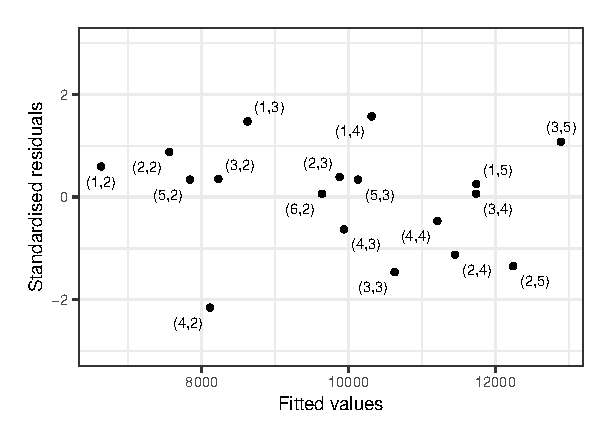
\includegraphics[scale=0.9]{original_resids}
  \caption{Diagnostic plot for original triangle}
  \label{fig:diag-plot-original}
\end{figure}

The same diagnostic plots are shown in \cref{fig:diag-plot-perturbed} for the case where the points $(2, 5)$ and $(4, 4)$ have been perturbed by a factor $1.5$, either by direct multiplication or through simulation from the underlying model. The residual corresponding to the pathological observation has been highlighted in red. As these examples demonstrate, it is not always feasible to identify deviations from the model assumptions by examining such plots, even for the trained eye.

\begin{figure}[!htb]
  \centering
  \begin{subfigure}{\textwidth}
    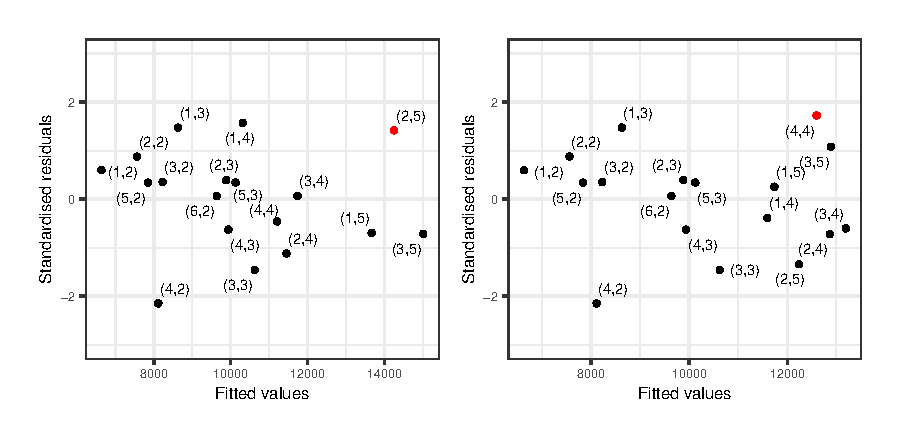
\includegraphics{perturbed_resids}
    \caption{Perturbed directly}
  \end{subfigure}
  \begin{subfigure}{\textwidth}
    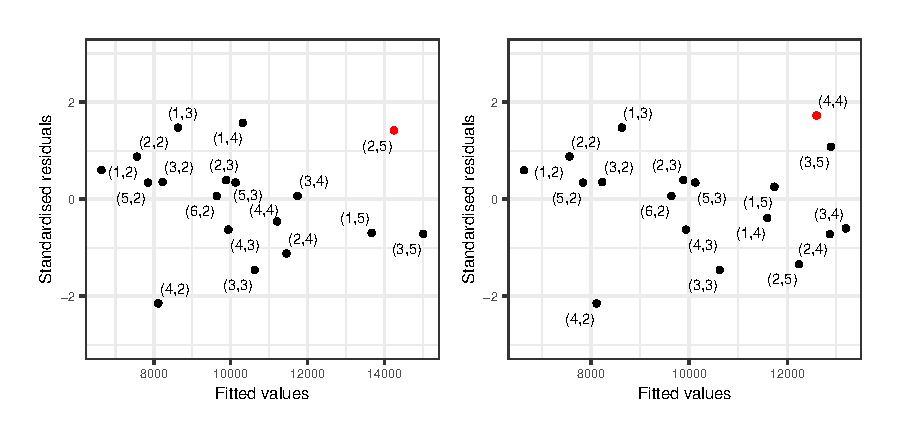
\includegraphics{model_perturbed_resids}
    \caption{Perturbed according to model}
  \end{subfigure}
  \caption{Diagnostic plots for perturbed triangles}
  \label{fig:diag-plot-perturbed}
\end{figure}

Our aim is to investigate whether it is possible to use bootstrap simulations to remedy this problem. The text is divided as follows. The next chapter introduces the bootstrap and explains how it can be used for inference on regression models, which is how we will frame the reserving methods under consideration. In the following two chapters, we will then apply this theory to the most widespread stochastic claims reserving models, \modelref{model:mack} and \modelref{model:odp}, in order to study whether it is possible to identify pattern breaks using bootstrap simulation. Specifically, we simulate claims triangles which perfectly follow the model assumptions, perturb these, and generate a bootstrap reserve from the resulting dataset. This will allow us to investigate how the simulated reserve is impacted by deviations from the model assumptions.

\mainmatter%

\chapter{The bootstrap method} \label{chapter:boot}

When using a statistical model to describe a dataset in terms of a reduced number of parameters, we are not only interested in producing point estimates of these parameters, but also in quantifying their \emph{uncertainty}. In classical statistics, the usual approach to achieve this is to start from the model assumptions and derive from them analytically the sampling distribution of the estimators. In most cases (the Gaussian distribution being a notable exception) this leads to intractible calculations, so that one is either forced to rely on approximations and asymptotic results, or make unrealistic simplifying assumptions. Moreover, estimates obtained in this way often heavily depend on their underlying assumptions, which can potentially lead to gross errors if these are violated.

The bootstrap method aims to remedy this problem by using numerical simulations to compute estimates of model uncertainty. At its core, it is premised on the idea that the empirical distribution of the sample forms a good proxy for that the population distribution. Consequently, we can approximate sampling from the population by \emph{resampling our data}, which, to the uncareful observer, can give the impression that we're 'magically' producing new information, using our single sample to 'pull ourselves up by our own bootstraps', which is where the procedure derives its name from. Let's see how this can be done concretely for a simple estimation problem.

\section{Bootstrapping an estimator}

Let $X_1, \dots, X_n$ be an i.i.d. sample drawn from a distribution $F$, and consider an estimator $\widehat{h(F)} = g(X_1, \dots, X_n)$ of some quantity $h(F)$ whose uncertainty we wish to estimate using e.g.\ the variance of the sampling distribution. Depending on the assumptions we are willing to make, we can choose between two broad approaches: \emph{parameteric} methods and \emph{nonparametric} ones.

In the nonparametric bootstrap, we use the data directly, drawing with replacement to simulate new samples $X^{(b)}_1, \dots, X^{(b)}_n$. In other words, we approximate $F$ using the \emph{empirical cumulative distribution function}
\begin{equation}
  \widehat{F}_n(x) \coloneqq \sum_{k=1}^n I_{\{ X_k \leq x \}} \,,
\end{equation}
which we use to generate new data. We then compute the statistic of interest on these pseudo-samples, yielding pseudo-observations $g^{(b)} = g(X^{(b)}_1, \dots, X^{(b)}_n)$ which approximate the sampling distribution of $\widehat{h(F)}$. Writing $B$ for the total number of bootstrap samples, we can esimate the variance of $\widehat{h(F)}$ by
\begin{equation}
  \frac{1}{B-1}\sum_{b=1}^B(g^{(b)} - \bar{g})^2 \,,
\end{equation}
with $\bar{g} = \frac{1}{B} \sum_{b=1}^B g^{(b)}$. Provided $F \approx \widehat{F}_n$ holds with sufficient accuracy, this will yield a reasonable approximation to $\mathrm{Var}(\widehat{h(F)})$.

By contrast, in the parametric bootstrap, we first fit a model using the data, and then simulate samples from this with the help of a random number generator. As usual, the parametric approach offers the advantage of efficiency if its assumptions are met, at the risk of increased error when they are violated. If we assume that $F$ belongs to some family $\left \{ F_{\bm{\theta}} \mid  \bm{\theta} \in \Theta \right \}$, then we can use the sample $X_1, \dots, X_n$ to produce an estimate $\bm{\widehat{\theta}}$ of the parameter. Plugging this in then gives us $F_{\bm{\widehat{\theta}}}$, from which we can simulate $X^{(b)}_1, \dots , X^{(b)}_n$ and $g^{(b)}$ as before. An estimate of the sampling variance can be obtained the same manner.

Although we have thus far only used it for the calculation of a single statistic, it is clear that the bootstrap produces a complete \emph{simulated distribution} of the estimator, which can be used for many different forms of inference. This highlights its tremendous potential as a tool for statistical analysis, which explains the rise in popularity of bootstrap methods once personal computers powerful enough to carry out the requisite calculations became widely available. Let us give an example to illustrate this. \cref{fig:boot-est} compares, for a $\Gamma(\alpha, \beta)$-distribution with $\alpha = 2$ and $\beta = 0.5$, the bootstrap distributions of the maximum likelihood estimators to their exact counterparts. It is clear that the bootstrap distribution approaches the analytic one. We use a simulated sample of size $n = 1000$ and compute . The analytic distributions are based on the well-known fact from likelihood theory that the asymptotic distribution of the MLE is given by the multivariate normal distribution $\mathcal{N}(\bm{\theta}, I(\bm{\theta})^{-1})$, where $\bm{\theta}$ is the parameter vector and $I(\bm{\theta})$ the Fisher information matrix. For the gamma distribution, the latter is given by
\begin{equation}
  I(\alpha, \beta) = n
  \begin{pmatrix}
    \psi'(\alpha) & -1 / \beta       \\
    -1 / \beta    & \alpha / \beta^2
  \end{pmatrix} \,
\end{equation}
where $\psi(x) \coloneqq \odv{}{x} \log \Gamma(x)$ is the so-called digamma function.

\begin{landscape}
  \begin{figure}
    \begin{subfigure}{\linewidth}
      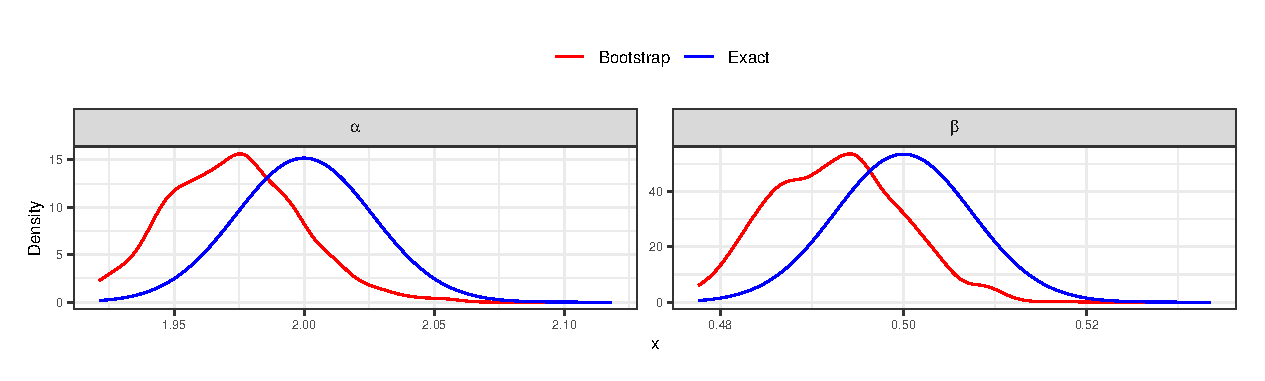
\includegraphics{boot_est_param}
      \subcaption{Parametric}
    \end{subfigure}
    \begin{subfigure}{\linewidth}
      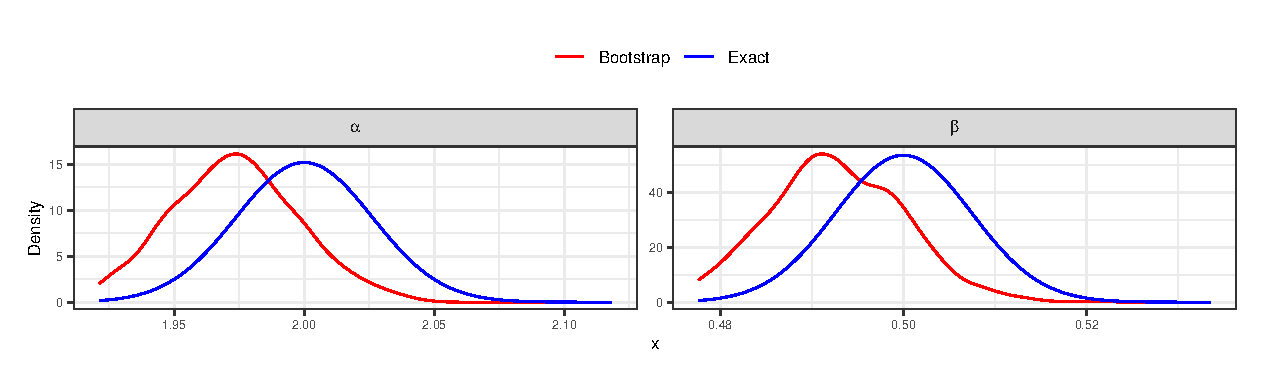
\includegraphics{boot_est_nonparam}
      \subcaption{Nonparametric}
    \end{subfigure}
    \caption{Analytic and bootstrap distribution of MLE for a gamma distribution with $\alpha = 2$ and $\beta = 0.5$}
    \label{fig:boot-est}
  \end{figure}
\end{landscape}

\section{Bootstrapping a regression model} \label{sec:boot-reg}

Altough we have introduced the bootstrap in the context of a classical one-sample estimation problem, the same principles can be applied to data structures of arbitrary complexity, so long as we have a model for the probabilistic mechanism generating the observations (see \cite[Chapter 8]{efron:intro} for a general exposition of this methodology). In particular, bootstrap methods for regression models are well-established in the literature. We now turn our attention to these, as they will form the foundation for developing bootstrap methods for claims triangles.

Consider a set of covariates $X_1, \dots, X_p$ and a response variable $Y$ whose relationship we model by a parametrised mapping $f(X_1, \dots, X_p; \bm{\beta})$. Given a sample of pairs $(\bm{\mathrm{x}_1}, Y_1), \dots, (\bm{\mathrm{x}_n}, Y_N)$ and a choice of loss function, we can fit this model to obtain an estimate $\widehat{\bm{\beta}}$ of $\bm{\beta}$. For new values $x_1^+, \dots, x_N^+$ of the regressors, we can then predict the response $Y^+$ as $f(x_1^+, \dots, x_N^+; \widehat{\bm{\beta}})$. It is worth emphasising these as two distinct operations, which correspond to different bootstrap procedures (see \cite[Sections 6.3.3 and 7.2.4]{davison}). \emph{Estimation} seeks to \emph{identify} the value of a quantity which is \emph{fixed but unknown}; \emph{prediction} aims to \emph{forecast} the value of a \emph{random variable}.

Under the least squares criterion, for example, we know that the optimal predictor for $Y$ is the conditional expectation $\condexp{Y}{X = x}$. This is an ordinary function which returns a real number for any $x \in \mathbb{R}^p$, and which can therefore be estimated from a sample. Such an estimate will contain some error, which we have to take into account when doing inference. If we additionally want to measure the error we make when predicting $Y$ using $\condexp{Y}{X = x}$, we also have to incorporate the intrinsic randomness or \emph{process variance} of the response variable. Prediction is therefore a two-stage procedure involving an intermediate estimation step.

Let's illustrate this in the case of the all-familiar linear regression model, which is given by
\begin{equation} \label{eq:linear-model}
  Y_i = \bm{\mathrm{x}_i}^T \bm{\beta} + \varepsilon_i \,, \qquad i \in {1, \dots, n}
\end{equation}
with $\expect{\varepsilon_i} = 0$, $\operatorname{Var}(\varepsilon_i) = \sigma$ and $\expect{\varepsilon_i \varepsilon_j} = 0$ for $i \neq j$. Considering the nonparametric bootstrap first, we need to identify a fundamental unit of resampling such that the resulting variables are interchangeable. One option would be to use some suitably standardised residuals which we obtain by fitting the model (see \cite[Algorithm 6.1]{davison}). This approach is sometimes referred to as \emph{semiparametric}, because it only uses the specification of certain aspects of the data distribution in terms of some parameters, but does not assume a specific form for it. Choosing, for example, the residuals
\begin{equation}
  r_i \coloneqq \frac{Y_i - \bm{\mathrm{x}}^T_i \widehat{\bm{\beta}}}{\widehat{\sigma} \sqrt{1 - h_{ii}}} \,,
\end{equation}
we resample these for $B$ times to obtain pseudo-residuals $r^{(b)}_1, \dots, r^{(b)}_n$, which in turn yield  pseudo-responses
\begin{equation}
  Y_i^{(b)} \coloneqq \mathbf{x}^T \widehat{\bm{\beta}} + \widehat{\sigma} r^{(b)}_i \,.
\end{equation}
By refitting the model to this new pseudo-data, we then obtain bootstrapped regression parameter estimates $\widehat{\bm{\beta}}^{(b)}$ for $1, \dots, B$.

An alternative approach, which is fully nonparametric, is to resample the pairs $(\bm{\mathrm{x}_i}, Y_i)$ themselves (see \cites[Section 9.5]{efron:intro}[Algorithm 6.2]{davison}), which corresponds to approximating the multivariate distribution of $(X_1, \dots, X_n, Y)$ by the empirical distribution of the data. This has the significant benefit of parsimony, making no other assumption beside the i.i.d.-ness of the sample. The model is then fitted to the bootstrap samples $(\bm{\mathrm{x}_1}^{(b)}, Y^{(b)}_1), \dots, (\bm{\mathrm{x}_n}^{(b)}, Y^{(b)}_n)$ to produce pseudo-realisations $\widehat{\bm{\beta}}^{(b)}$ of the regression parameter estimator.

For the parametric case, we have to make an additional assumption about the distribution of $\epsilon$, the classical choice being the Gaussian one.

We then  to fit \cref{eq:linear-model}, which gives us estimates $\widehat{\beta}$ for the regression parameters.

With the help of a random number generator, we then produce bootstrap responses $Y^{(b)}_1, \dots, Y^{(b)}_n$ by drawing from the estimated distribution $\mathcal{N}(\bm{\mathrm{x}}^T \widehat{\bm{\beta}}, \widehat{\sigma}^2)$, and fit the model to this new data to obtain bootstrap samples $\widehat{\bm{\beta}}^{(b)}$ of the regression parameters.

\section{Process variance and predictive distributions} \label{sec:boot-proc}

If we want to do predictive inference on a regression model using the bootstrap, we additionally have to take into account the inherent variability of the response. Considering once again the example of the normal linear model, suppose we are interested in predicting the response $Y_+$ at new value $\mathbf{x_+}$ of the regressors. One way to quantify the accuracy of our forecast is to consider the \emph{prediction error}
\begin{equation}
  \delta \coloneqq Y_+ - \widehat{Y}_+
\end{equation}
(see \cite[Algorithm 6.4]{davison}). The second term in this expression can be bootstrapped using any one of the methods described in the previous section, as these yield replicates $\widehat{\bm{\beta}}^{(b)}$ of the parameter estimator and hence of the predictor $\widehat{Y}^{(b)}_+ = \mathbf{x_+}^T \widehat{\bm{\beta}}^{(b)}$. It then remains for us to produce bootstrap simulations of the response $Y_+$ itself. In the semiparametric approach, this can be achieved by resampling the residuals a second time to obtain pseudo-realisations $r^{(s)}$ for $s = 1, \dots, S$, and adding these (after correctly scaling them) to the value of the regression line at $x_+$. The resulting pseudo-responses $Y^{(s)}_+$ mimick the random fluctuations of $Y_+$, allowing us to approximate $\delta$ with the bootstrapped prediction errors
\begin{equation} \label{eq:pred-error-boot}
  \widehat{\delta}^{(b, s)} \coloneqq Y^{(s)}_+ - \widehat{Y}^{(b)}_+ = (\widehat{\mathbf{x}}^T_+ \widehat{\bm{\beta}} + r^{(s)}) - \widehat{\mathbf{x}}^T_+ \widehat{\bm{\beta}}^{(b)} \,.
\end{equation}
A similar procedure can be outlined for the parametric bootstrap by appropriately adjusting the method of generating bootstrap response replicates. The method cannot be applied to the pairs bootstrap, however, as it lacks a mechanism for simulating new response values by themselves; we must therefore borrow this part from one of the alternative approaches, forsaking part of its parsimony and robustness properties in the process. We can then use \cref{eq:pred-error-boot} for different kinds of inference, e.g. obtaining prediction intervals or estimating the mean squared error of prediction.

While this offers an avenue for incorporating the process variance into bootstrap procedures for predictive inference, it is not the one best suited to our purposes. Recall from the \nameref{intro} that we want to study how the reserve is impacted by violations of the assumptions of a given actuarial model which can be framed in terms of regression, as we shall see in \cref{chapter:mack,chapter:poisson}. In other words, we would like to simulate the distribution of the response itself. In \cref{eq:pred-error-boot}, this was done by generating fluctuations around $\widehat{\bm{\beta}}$ through resampling (or in the parametric case, with the help of a random number generator). The trouble with this approach is that it fails to account for the error in our parameter estimates, leading to an underestimation of the prediction uncertainty. Although we will endeavour in this exposition to remain agnostic with respect to philosophical questions about the interpretation of probability, it will be necessary in this case, for reasons which will become apparent shortly, to borrow a concept from Bayesian school of statistics in order to address this problem.

Recall that the Bayesian point of view is premised on the idea that the parameters $\bm{\theta}$ governing a statistical model $p(y \mid \bm{\theta}, x_1, \dots, x_p)$ are themselves random variables. These are assumed to follow a so-called \emph{prior distribution} $p(\theta)$, which is a probabilistic expression of the beliefs we have about them before observing any data\sepfootnote{fn:bayes}. When presented with a sample $D = \{ (\bm{\mathrm{x}_1}, Y_1), \dots, (\bm{\mathrm{x}_n}, Y_n) \}$, we are then led to \emph{update our beliefs}; using the formula
\begin{equation}
  p(\bm{\theta} \mid D) \propto p(D \mid \bm{\theta}) p(\bm{\theta}) \,,
\end{equation}
which is known as \emph{Bayes' rule}, we obtain the \emph{posterior distribution} $p(\bm{\theta} \mid D)$ expressing the likelihood of different values of $\bm{\theta}$ given our observations. For any value of the parameters, the likelihood of the response at a new input, conditional on this value and the sample $D$, is now given by $p(y_+ \mid \bm{\theta}, D)$. By marginalising over the posterior distribution, we then incorporate all possible values of $\bm{\theta}$ in proportion to their likelihood under the data, resulting in the \emph{posterior predictive distribution}.
\begin{equation}
  p(y_+ \mid D) = \int p(y_+ \mid \bm{\theta}) p(\bm{\theta} \mid D) \, d \bm{\theta} \,.
\end{equation}
of $Y_+$ given $D$. This incorporates both the intrinsic variability of the response as well as our uncertainty regarding the parameters (or, in the classical view, their estimates). By contrast, \emph{fitted distribution} $p(y_+ \mid \widehat{\bm{\theta}})$, obtained by plugging in some estimate of the parameters, does not have this virtue. Moreover, the predictive distribution can be very easily integrated into the bootstrap framework. Indeed, we can follow the same steps as when simulating the prediction errror, but instead of \cref{eq:pred-error-boot}, we compute pseudo-realisations
\begin{equation} \label{eq:pred-dist}
  Y_+^{(b, s)} \coloneqq \mathbf{x}_+^T \widehat{\bm{\beta}}^{(b)} + \widehat{\sigma} r^{(s)} \,.
\end{equation}
\cref{eq:pred-dist} also explains why it is difficult to fit this approach within a classical frequentist paradigm, as it is unclear in that case which theoretical quantity these bootstrap replicates would be approximating. We hasten to add that much work has been done to remedy this, leading, among other things, to the concept of a \emph{confidence distribution} (see, for example, \cites{barndorff-nielsen,lawless}). It is true, however, that there has been a multiplicity of disparate frequentist versions of the predictive distribution, as remarked for instance by \textcite{dickson}, lending credence to the idea that the notion fits more naturally into the Bayesian framework.

In order to illustrate the difference between fitted and predictive distributions, we also introduce a bootstrap definition for the former. This only differs from \cref{eq:pred-dist} in that it uses the original parameter estimate rather than the bootstrap one:
\begin{equation} \label{eq:fit-dist}
  Y_+^{(s)} \coloneqq \mathbf{x}_+^T \widehat{\bm{\beta}} + \widehat{\sigma} r^{(s)} \,.
\end{equation}
We also note that the notions of predictive and fitted distribution originate in mathematical statistics, where the goal is to derive analytical expressions for them; in this text, we shall always understand them to refer to their bootstrap equivalents. For the following example, we consider a normal linear model with $p = 10$, $n = 1000$, $\sigma = 5.7$ and
\begin{displaymath}
  \bm{\beta} = \begin{bmatrix} 4.1 & 4.4 & -2.1 & 3.3 & 1.4 & 0.2 & 2.4 & -3.7 & 1.6 & 2.1 \end{bmatrix} \,.
\end{displaymath}
The predictive and fitted distributions for both the parametric as well as non-parametric bootstrap are is shown in \cref{fig:boot-reg}. We can see in this case that the two are nigh indistinguishable, which is presumably due to the fact that the data are simulated and thus follow the model perfectly. As we shall see in \cref{sec:mack-proc}, we will not encounter such perfect agreement with the claims reserving models.

\begin{figure}[!htb]
  \begin{subfigure}{\linewidth}
    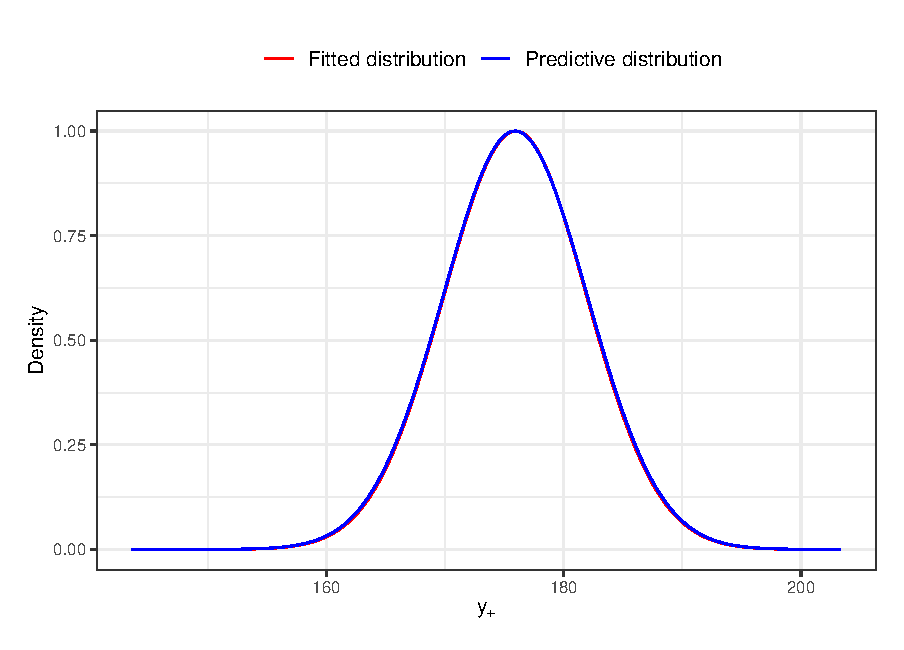
\includegraphics{boot_reg_param}
    \subcaption{Parametric}
  \end{subfigure}
  \begin{subfigure}{\linewidth}
    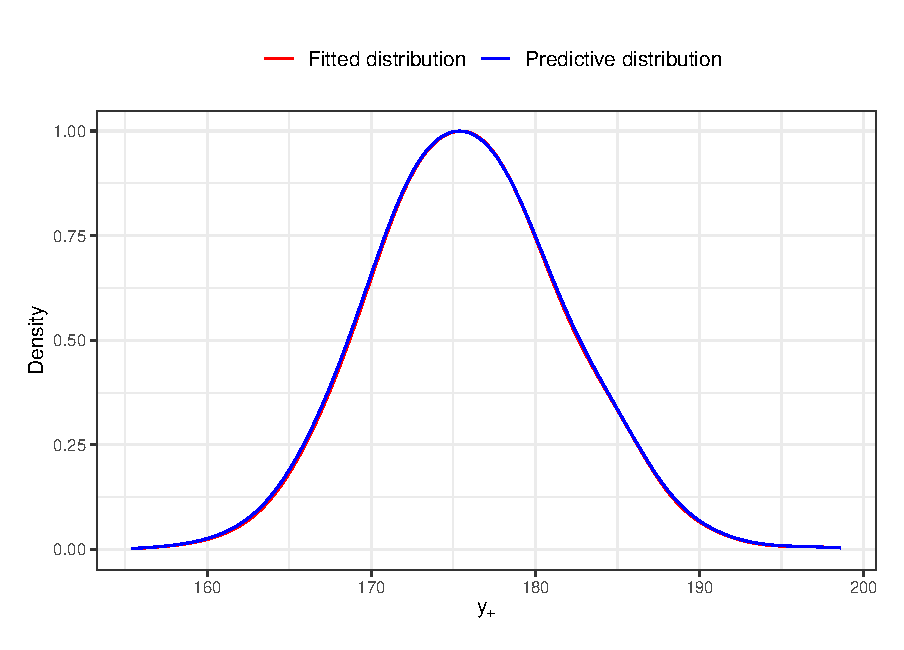
\includegraphics{boot_reg_semiparam}
    \subcaption{Semiparametric}
  \end{subfigure}
  \caption{Comparison of the fitted and predictive bootstrap distributions for a normal linear model}
  \label{fig:boot-reg}
\end{figure}

\chapter{Mack's model} \label{chapter:mack}

\section{Introduction} \label{sec:mack-intro}

In his seminal paper \cite{mack:chain-ladder}, Mack proposed the following model for cumulative claims triangles, which remains among the most influencial in actuarial reserving.
\begin{model}[Mack chain ladder] \label{model:mack} \leavevmode
  \begin{enumerate}[label=\bf{\textup{(}Mack\arabic*\textup{)}},ref=\textup{(}Mack\arabic*\textup{)}, wide]
    \item \label{assump:mack-expectation} There exist development factors $f_1, \dots, f_{I - 1}$ such that
          \begin{equation}
            \mathbb{E}[C_{ij} \ \Vert \ C_{i, j - 1}, \dots, C_{i1}] = \mathbb{E}[C_{ij} \ \Vert \ C_{i, j - 1}] = f_{j - 1} C_{i, j - 1}\,
          \end{equation}
          for $1 \leq i \leq I$.
    \item \label{assump:mack-variance} There exist parameters $\sigma_1, \dots, \sigma_{I - 1}$ such that
          \begin{equation}
            \mathrm{Var}[C_{ij} \ \Vert \ C_{i, j - 1}, \dots, C_{i1}] = \mathrm{Var}[C_{ij} \ \Vert \ C_{i, j - 1}] = \sigma_{j - 1}^2 C_{i, j - 1}\,,
          \end{equation}
          for $1 \leq i \leq I$.
    \item \label{assump:mack-independence} Cumulative claims processes $(C_{ij})_j, (C_{i'j})_j$ are independent for $i \neq i'$.
  \end{enumerate}
\end{model}
The development factors are estimated by
\begin{equation} \label{eq:devfac-estimator}
  \widehat{f}_j(\mathcal{D}_I) = \widehat{f}_j(C_{1j}, \dots, C_{I - j, j}, \dots, C_{1, j + 1}, \dots, C_{I - j, j + 1}) \coloneqq \frac{\sum_{i = 1}^{I - j} C_{i, j + 1}}{\sum_{i = 1}^{I - j} C_{i, j}} \,.
\end{equation}
If we define the \emph{single} or \emph{individual} development factors as
\begin{equation}
  F_{i, j + 1} \coloneqq \frac{C_{i, j + 1}}{C_{ij}} \,,
\end{equation}
then $\widehat{f}_j$ can be obtained as the weighted average
\begin{equation}
  \widehat{f}_j = \frac{\sum_{i = 1}^{I - j} C_{ij} F_{i, j}}{\sum_{i = 1}^{I - j} C_{ij}} \,.
\end{equation}
The $\sigma_j$ are estimated by
\begin{equation}
  \widehat{\sigma}_j \coloneqq \frac{1}{I-j}\sum_{i = 1}^{I-j} C_{ij}\left( F_{i, j + 1} - \widehat{f}_j \right)^2
\end{equation}
for $j < I - 1$. This formula does not work for $j = I - 1$, as we only have a single pair of observations in the last two columns of the triangle. To remedy this, Mack proposed a simple extrapolation from the previous development years, leading to the estimate
\begin{equation}
  \widehat{\sigma}^2_{I - 1} = \min{ \left \{ \frac{\widehat{\sigma}^4_{I - 2}}{\widehat{\sigma}^2_{I - 3}}, \widehat{\sigma}^2_{I - 2}, \widehat{\sigma}^2_{I - 3} \right \} }
\end{equation}
and this appears to be the most widely adopted solution in the literature.

Under the assumptions of \modelref{model:mack}, it can be shown (see \cite[17 \psqq]{wuthrich:stochastic-reserving}) that $\widehat{f}_j$ and $\widehat{\sigma}_j$ are (conditionally) unbiased, and moreover that the $\widehat{f}_j$ are uncorrelated. Predicted ultimate claim amounts $C_{iI}$ are obtained by substituting the estimates for the unknown development factors $f_j$ in the conditional expectation. In other words, we predict the ultimate loss using the conditional mean $\condexpp{C_{iI}}{C_{i, I + 1 - i}}$, and estimate the latter by plugging in $\widehat{f}_j$, yielding
\begin{equation}
  \widehat{C}_{iI} \coloneqq \widehat{\mathbb{E}}[C_{i, I} \ \Vert \ C_{i, I - i}] = C_{i, I + 1 - i} \prod_{j = I - i}^{I-1} \widehat{f}_j \,.
\end{equation}
From this, we then finally obtain the reserve predictor
\begin{equation} \label{eq:reserve-predictor}
  \widehat{R} = g(\mathcal{D}_I) \coloneqq \sum_{i = 2}^I (\widehat{C}_{i, I} - C_{i, I + 1- i}) \,.
\end{equation}

\Modelref{model:mack} is often referred to as "distribution-free" because it only makes assumptions about the first two moments of the claims triangle variables. Indeed, we will show that \modelref{model:mack} can be viewed as a series of linear regressions through the origin (i.e.\ without intercept term), hence these are same assumptions as for the Gauss-Markov theorem, i.e. the minimal ones\sepfootnote{fn:gauss-markov} required to guarantee optimality. Introduce, for any development year $j \in \{ 1, \dots, {I - 1} \}$, the notation
\begin{equation}
  \bm{\mathrm{c}_j} \coloneqq
  \begin{bmatrix}
    C_{1, j} \\
    \vdots   \\
    C_{I - j, j}
  \end{bmatrix} \,,
\end{equation}
then the first two assumptions of \modelref{model:mack} can be equivalently stated as
\begin{equation}
  \bm{\mathrm{c}_{j + 1}} = f_j \bm{\mathrm{c}_j} + \bm{\varepsilon} \,,
\end{equation}
with $\bm{\varepsilon}$ a random vector satisfying
\begin{equation}
  \condexpp{\bm{\varepsilon}}{C_{1, j}, \dots, C_{i, I - j}} = \bm{0}
  \qquad%
  \condvarr{\bm{\varepsilon}}{C_{1, j}, \dots, C_{i, I - j}} = \sigma^2_j
  \begin{bmatrix}
    C_{1j} &        &              \\
           & \ddots &              \\
           &        & C_{I - j, j}
  \end{bmatrix} \,.
\end{equation}
Consequently, it follows (see \cite[Proposition 1.7]{hayashi}) that the weighted least squares method with weights matrix
\begin{equation}
  \mathbf{W} =
  \begin{bmatrix}
    1 / C_{1j} &        &                  \\
               & \ddots &                  \\
               &        & 1 / C_{I - j, j}
  \end{bmatrix} \,,
\end{equation}
leads to an estimator for $f_j$ which has minimal variance in the class of linear unbiased estimators. This estimator is given by
\begin{equation}
  \widehat{f}^{\mathrm{WLS}}_j = (\bm{\mathrm{c}_j}^T \mathbf{W} \bm{\mathrm{c}_j})^{-1} \bm{\mathrm{c}_j}^T \mathbf{W} = \frac{\sum_{i = 1}^{I - j} C_{i, j + 1}}{\sum_{i = 1}^{I - j} C_{i, j}} \,,
\end{equation}
which is the same expression as \cref{eq:devfac-estimator}.

\section{A challenging simulation} \label{sec:mack-challenge}

Owing to its recursive nature, Mack's model does not readily lend itself to application of the theory from \cref{chapter:boot}. The actuarial literature on bootstrap methods is not very helpful in this regard either, as it has mostly tended to focus on generalised linear models---even papers like \cite{england:dist} which address \modelref{model:mack} do so by reframing it in this way. As will become clear shortly, this passes over some subtleties related to the particular structure of Mack's model, and we will therefore take a different approach. In particular, our starting point will be the problem of deriving a closed-form estimate of the so-called conditional \emph{mean square error of prediction} (MSEP) for the Mack predictor. While this might appear at first glance to be unrelated to the bootstrap, we will see that it furnishes us with the necessary theoretical framework to understand the special issues involved in resampling a recursive model.

The MSEP is a measure for the total uncertainty associated with a given predictive model. It is defined as the Euclidean distance between the predictor and the response in the underlying filtered probability space, i.e.\
\begin{equation}
  \underset{R \, \vert \, \mathcal{D}_I}{\mathrm{MSEP}}(\widehat{R}) \coloneqq \condexpp*{(\widehat{R} - R)^2}{\mathcal{D}_I}
\end{equation}
for our special case of predicting the reserve. The MSEP admits a decomposition, similar to the familiar bias-variance decomposition from classical statistics into so-called \emph{parameter} or \emph{estimation error} and \emph{process error}:
\begin{align}
  \begin{split}
    \condexpp*{(\widehat{R} - R)^2}{\mathcal{D}_I} &= \condexpp*{(R - \condexpp*{R}{\mathcal{D}_I})^2}{\mathcal{D}_I} + \condexpp*{(\condexpp*{R}{\mathcal{D}_I} - \widehat{R})^2}{\mathcal{D}_I} \\ &\phantom{{}=1} -2\condexpp*{(R - \condexpp*{R}{\mathcal{D}_I})(\condexpp*{R}{\mathcal{D}_I} - \widehat{R})}{\mathcal{D}_I}
  \end{split} \\
  \begin{split}
    &= \mathrm{Var}(R \, \Vert \, \mathcal{D}_I) + (\condexpp*{R}{\mathcal{D}_I} - \widehat{R})^2 \\
    &\phantom{{}=1} -2(\condexpp*{R}{\mathcal{D}_I} - \widehat{R})(\condexpp*{R - \condexpp*{R}{\mathcal{D}_I}}{\mathcal{D}_I})
  \end{split}                                                                                                                                                                                                                                               \\
   & = \underbrace{\mathrm{Var}(R \, \Vert \, \mathcal{D}_I)}_\text{process error} + \underbrace{(\condexpp*{R}{\mathcal{D}_I} - \widehat{R})^2}_\text{estimation error} \,,
\end{align}
corresponding to the two stages of bootstrapping a predictor which we discussed in \cref{sec:boot-reg}. Consider now, for any accident year $i \in \{ 1, \dots, I \}$, the MSEP for the associated ultimate
\begin{equation} \label{eq:msep}
  \underset{C_{iI} \, \vert \, \mathcal{D}_I}{\mathrm{MSEP}}(\widehat{C}_{iI}) = (\condexpp*{C_{iI}}{\mathcal{D}_I} - \widehat{C}_{iI})^2 + \condvarr{C_{iI}}{\mathcal{D}_I} \,,
\end{equation}
and suppose we are interested in obtaining a closed-form estimator for it. Such an expression can be derived relatively straightforwardly for the process error from the assumptions of \modelref{model:mack} in the following way. We begin by applying the law of total variance in conjunction with \cref{assump:mack-expectation,assump:mack-variance} to obtain
\begin{align}
  \condvarr{C_{iI}}{\mathcal{D}_I} & = \condvarr{C_{iI}}{C_{i, I + 1 - i}}                                                                                             \\
                                   & = \condexpp{\condvarr{C_{iI}}{C_{i, I - 1}}}{C_{i, I + 1 - i}} + \condvarr{\condexpp{C_{iI}}{C_{i, I - 1}}}{C_{i, I + 1 - i}}     \\
                                   & = \sigma^2_{I - 1} \condexpp{C_{i, I - 1}}{C_{i, I + 1 - i}} + f^2_{I - 1} \condvarr{C_{i, I - 1}}{C_{i, I + 1 - i}}              \\
                                   & = \sigma^2_{I - 1} C_{i, I + 1 - i} \prod_{j = I + 1 - i}^{I - 2} f_j + f^2_{I - 1} \condvarr{C_{i, I - 1}}{C_{i, I + 1 - i}} \,,
\end{align}
which is a linear recurrence equation of the form
\begin{equation}
  x_n = a_{n - 1} x_{n - 1} + g_{n - 1}
\end{equation}
with $x_n = \condvarr{C_{in}}{C_{i, I + 1 - i}}$ and
\begin{equation}
  g_{n - 1} = \sigma^2_{n - 1} C_{i, I + 1 - i} \prod_{j = I + 1 - i}^{n - 1} f_j \,, \qquad a_{n - 1} = f^2_{n - 1} \,.
\end{equation}
The general solution is given by
\begin{equation}
  x_n = \left( \prod_{j = n_0}^{n - 1} a_j \right) \left( x_{n_0} + \sum_{k = n_0}^{n - 1} \frac{g_k}{\prod_{l = n_0}^k a_l} \right)
\end{equation}
where $n_0$ denotes the first index of the sequence $x_n$, in our case $I + 1 - i$. Using the initial condition $x_{I + 1 - i} = \condvarr{C_{i, I + 1 - i}}{C_{i, I + 1 - i}} = 0$, we finally obtain
\begin{align}
  \condvarr{C_{iI}}{\mathcal{D}_I}
   & = \left( \prod_{j = I + 1 - i}^{I - 1} f^2_j \right) \left( \sum_{k = I + 1 - i}^{I - 1} \frac{\sigma^2_k C_{i, I + 1 - i} \prod_{j = I + 1 - i}^{k - 1} f_j}{\prod_{j = I + 1 - i}^k f^2_j} \right) \\
   & = \left( \prod_{j = I + 1 - i}^{I - 1} f^2_j \right) C^2_{i, I + 1 - i} \left( \sum_{k = I + 1 - i}^{I - 1} \frac{\sigma^2_k / f^2_k}{\prod_{j = I + 1 - i}^{k - 1} f_j C_{i, I + 1 - i}} \right)    \\
   & = \condexpp{C_{iI}}{C_{I + 1 - i}}^2 \sum_{k = I + 1 - i}^{I - 1} \frac{\sigma^2_k / f^2_k}{\condexpp{C_{ik}}{C_{i, I + 1 - i}}} \,,
\end{align}
which we can estimate by plugging in $\widehat{f}_j$ and $\widehat{\sigma}_j$ for $f_j$ and $\sigma_j$, respectively.

For the parameter error, if we use the definitions from the previous section to rewrite it as
\begin{align} \label{eq:param-err}
  (\condexpp*{C_{iI}}{\mathcal{D}_I} - \widehat{C}_{iI})^2 & = C^2_{i, I+1-i} \left( \prod_{j=I+1-i}^{I-1}f_j - \prod_{j=I+1-i}^{I-1}\widehat{f}_j \right)^2                                                  \\
                                                           & = C^2_{i, I+1-i} \left( \prod_{j=I+1-i}^{I-1}f^2_j + \prod_{j=I+1-i}^{I-1}\widehat{f}^2_j - 2 \prod_{j=I+1-i}^{I-1}f_j \widehat{f}_j \right) \,,
\end{align}
it becomes clear that things are more complicated than with process error. Indeed, we cannot simply subtitute the $\widehat{f}_j$ for the unknown parameters in this expression as that would cause it to vanish, yielding an estimate which will generally not be accurate. This problem was recognised by Mack himself in \cite{mack:chain-ladder-variability}, and is caused by the fact that the claims triangle observations are used for both estimation and forecasting (see \cite[Section 2]{lindholm:msep} for a more general discussion). His suggested solution was to apply some kind of conditional averaging to the $\widehat{f}_j$. Ideally, one would like to condition on all available observations in $\mathcal{D}_I$, but the $\mathcal{D}_I$-measurability of the $\widehat{f}_j$ would then bring us right back where we started. We must therefore use a smaller set in order to allow $\widehat{f}_{I + 1 - i}, \dots, \widehat{f}_{I - 1}$ to fluctuate around $f_{I + 1 - i}, \dots, f_{I - 1}$. This corresponds to asking which other values $\widehat{f}_j$ could have taken, given that we fix a certain subset of the data---in other words, it's a resampling scheme on the parameter estimates. Thus, one can obtain an estimate of the parameter error by specifying a mechanism for generating new realisations of $\widehat{f}_j$ (see \cites{wuthrich:chain-ladder-msep}[44 \psqq]{wuthrich:stochastic-reserving}), with different mechanisms yielding different estimates. The literature uses this mostly as a theoretical device to facilitate analytical calculations; for the specific approach developed by Mack, it leads to the estimator
\begin{equation} \label{eq:mack-msep-estimator}
  \widehat{\mathrm{MSEP}}(\widehat{R_i}) \coloneqq \widehat{C}_{iI} \sum_{j = I + 1 - i}^{I - 1} \frac{\widehat{\sigma}^2_j}{\widehat{f}_j} \left( \frac{1}{\widehat{C}_{ij}} + \frac{1}{\sum_{i = 1}^{I - j} C_{ij}} \right)
\end{equation}
(see \cite[11]{mack:chain-ladder-variability}).
In this case, however, the theory happens to fit in perfectly with the resampling framework, and we can therefore employ it as a basis for bootstrap procedures. In the remainder of this section, we outline two approaches for estimating \cref{eq:param-err} and indicate the corresponding resampling methods.

Denote the subset of observations in $\mathcal{D}_I$ up to and including development year $k$ by
\begin{equation}
  \mathcal{B}_k \coloneqq \left \{ C_{ij} \in \mathcal{D}_I \mid j \leq k \right \} \,,
\end{equation}
and write
\begin{equation}
  \mathcal{D}^O_{I, k} \coloneqq \left \{ C_{ij} \in \mathcal{D}_I \mid j > I + 1 - k \right \}
\end{equation}
for its complement. One option would then be to take the conditional expectation of $\widehat{f}_j$ with respect to $\mathcal{B}_{I+1-i}$, leading to the estimate
\begin{align} \label{eq:uncond-param-err}
  \condexpp{(\condexpp{C_{iI}}{\mathcal{D}_I} - \widehat{C}_{iI})^2}{\mathcal{B}_{I+1-i}} & = C^2_{i, I+1-i} \condexpp*{\left( \prod_{j=I+1-i}^{I-1}f_j - \prod_{j=I+1-i}^{I-1}\widehat{f}_j \right)^2}{\mathcal{B}_{I+1-i}}      \\
                                                                                          & = C^2_{i, I+1-i} \left( \condexpp*{\prod_{j=I+1-i}^{I-1}\widehat{f}^2_j}{\mathcal{B}_{I+1-i}} - \prod_{j=I+1-i}^{I-1}f^2_j \right)\,,
\end{align}
where we used the fact that the $\widehat{f}_j$ are uncorrelated. This corresponds to averaging over the distribution of $\mathcal{D}^O_{I, k}$, or, expressed in terms of resampling, to generating new observations in the upper right triangle. Borrowing the nomenclature from \cite{wuthrich:chain-ladder-msep}, we call this the \emph{unconditional approach}. Alternatively, we could average each $\widehat{f}_j$ only over the observations after $j$. This is equivalent to fixing the denominator $\sum_{i = 1}^{I - j} C_{ij}$ in the development factor estimator \cref{eq:devfac-estimator} and allowing the numerator $\sum_{i = 1}^{I - j} C_{i, j + 1}$ to vary. Formally, it corresponds to taking the expectation with respect to the probability measure defined on $\mathcal{D}^O_{I, i}$ by
\begin{equation}
  \mathbb{P}^*_{\mathcal{D}_I}(\{ dz_{ij} \}_{i + j \leq I + 1}) \coloneqq \prod_{j = 1}^{I - 1} \prod_{i = 1}^{I - j}  \mathbb{P}_{C_{i, j + 1}}(dz_{i, j + 1} \mid C_{ij} = c_{ij}) \,,
\end{equation}
yielding the estimate
\begin{align}
  \expect[\mathbb{P}^*_{\mathcal{D}_I}]{(\condexpp{C_{iI}}{\mathcal{D}_I} - \widehat{C}_{iI})^2} & = C^2_{iI} \, \expect[\mathbb{P}^*_{\mathcal{D}_I}]{\left( \prod_{j=I+1-i}^{I-1}f_j - \prod_{j=I+1-i}^{I-1}\widehat{f}_j \right)^2}      \\
                                                                                                 & = C^2_{i, I+1-i} \left( \expect[\mathbb{P}^*_{\mathcal{D}_I}]{\prod_{j=I+1-i}^{I-1}\widehat{f}^2_j} - \prod_{j=I+1-i}^{I-1}f^2_j \right) \\
                                                                                                 & = C^2_{i, I+1-i} \left( \prod_{j=I+1-i}^{I-1} \condexpp*{\widehat{f}^2_j}{\mathcal{B}_j} - \prod_{j=I+1-i}^{I-1}f^2_j \right) \,.
\end{align}
We refer to this as the \emph{conditional approach}, and it corresponds to a scheme in which only the observations from the next period are resampled to produce a new realisation of the parameter estimate for the current period.

There has been some controversy about which of these approaches should be preferred, leading to the vigorous discussion found in \cite{wuthrich:chain-ladder-msep, mack:msep, gisler:msep, venter:msep}. As we will see in \cref{sec:mack-boot}, difference between the results which they produce is negligeable, and so the question is mainly of theoretical interest. Nevertheless, based on the previous exposition, it seems reasonable to prefer whichever method produces resampled parameter estimates approximating the original $\widehat{f}_j$ most closely. In particular, we note that these posses the following property, the proof of which can be found in \cite{mack:msep}.

\begin{theorem}
  The squares of two successive development factor estimates in \modelref{model:mack} are negatively correlated:
  \begin{equation}
    \mathrm{Cov}(\widehat{f}_j, \widehat{f}_{j - 1}) < 0 \,.
  \end{equation}
\end{theorem}

\noindent In the conditional approach, the resampled parameter estimates are independent by construction, and so they cannot incorporate this covariance structure. In light of this, it would appear that the unconditional scheme has slightly better theoretical properties. As the empirical difference between the two is minimal, however, the conditional version is a reasonable approximation to fall back on when needed. In the next section, we will see how both approaches give rise to a variety of different bootstrap methods.

\section{Bootstrap methodology} \label{sec:mack-boot}

In \cref{sec:boot-reg}, we introduced a taxonomy for the different kinds of bootstrap, distinguishing between the semiparameteric, nonparametric and parametric type. We now consider how each of these can be applied to \modelref{model:mack}. For comparison, \cref{tab:mack-bench} shows the results of applying \modelref{model:mack} with the estimator \cref{eq:mack-msep-estimator} to the dataset from \cref{tab:uk-motor}.

\begin{table}[!htb]
  \centering
  \begin{tabularx}{0.7\linewidth}{XXXXX}\toprule%
    $i \,/ \,j$ & $\widehat{f}^\mathrm{CL}_j$ & $\widehat{\sigma}^\mathrm{CL}_i$ & $\widehat{R}_i^\mathrm{CL}$ & $\widehat{\mathrm{MSEP}}(\widehat{R}_j)$ \\ \midrule
    \csvreader[
      head to column names,
    late after line =                                                                                                                                     \\
    ]{%
      ../results/example/mack_bench.csv
    }{}{%
    \idx        & \devfacs                    & \sigmas                          & \reserve                    & \prederror
    } \bottomrule%
  \end{tabularx}
  \caption{Mack CL results for UK Motor triangle}
  \label{tab:mack-bench}
\end{table}

For the semiparametric bootstrap, the crucial step is to find a suitable definition for the residuals which ensures that they are interchangeable. The distribution-free nature of the model makes this difficult, however, as it limits the statements we can make about the errors to the first two moments. We can resolve this in one of two ways. The first option would be to extrapolate from homogeneity of the first two moments to homogeneity of the distributions. In that case, the \emph{raw residuals}
\begin{equation}
  e_{i, j + 1} \coloneqq C_{i, j + 1} - \widehat{C}_{i, j + 1} = C_{i, j + 1} - \widehat{f}_j C_{ij}
\end{equation}
are not an option, as these suffer from heteroscedasticity,
\begin{equation}
  \condvarr{e_{i, j + 1}}{C_{ij}} = \sigma^2_j \left( C_{ij} - \frac{C^2_{ij}}{\sum_{i = 1}^{I - j} C_{ij}} \right) \,.
\end{equation}
We can address this by dividing out this variance, i.e. we consider the errors
\begin{equation}
  \varepsilon_{i, j + 1} \coloneqq \frac{C_{i, j + 1} - f_j C_{ij}}{\sigma_j \sqrt{C_{ij}} \sqrt{1 - \frac{C_{ij}}{\sum_{i = 1}^{I - j} C_{ij}}}} \,,
\end{equation}
which satisfy $\condexpp{\varepsilon_{i, j + 1}}{C_{ij}} = 0$ and $\condvarr{\varepsilon_{i, j + 1}}{C_{ij}} = 1$. Provided the sampling variability of the $\widehat{f}_j$ and $\widehat{\sigma}_j$ is not too bad (which is not obvious given the small sample sizes we're usually dealing with), the same should hold approximately for the corresponding residuals
\begin{equation}
  r_{i, j + 1} \coloneqq \frac{C_{i, j + 1} - \widehat{f}_j C_{ij}}{\widehat{\sigma}_j \sqrt{C_{ij}} \sqrt{1 - \frac{C_{ij}}{\sum_{i = 1}^{I - j} C_{ij}}}} \,,
\end{equation}
obtained by substituting these estimators. Note that the factor $\sqrt{1 - \frac{C_{ij}}{\sum_{i = 1}^{I - j} C_{ij}}}$ in the denominator corresponds to the leverage adjustment, as can be seen by computing the hat matrix:
\begin{align}
  \mathbf{H} & = \bm{\mathrm{c}_j} (\bm{\mathrm{c}_j}^T \mathbf{W} \bm{\mathrm{c}_j})^{-1} \bm{\mathrm{c}_j}^T \mathbf{W} \\[4pt]
             & = \frac{1}{\sum_{i = 1}^{I - j} C_{ij}}
  \begin{bmatrix}
    C_{1j}       & \dots  & C_{1j}       \\
    \vdots       & \ddots & \vdots       \\
    C_{I - j, j} & \dots  & C_{I - j, j}
  \end{bmatrix} \,.
\end{align}
It's worth emphasising, however, that the above extrapolation should not be made lightly, as it is perfectly possible for the error distribution to exhibit heterogeneity in other ways than through its mean and variance (see \cite[114]{efron:intro} for an example where the \emph{percentiles} vary with the value of the regressor). In light of this, an alternative approach would be to augment our model with some explicit distributional assumptions, which is more transparent and allows us to make precise statements about errors and residuals. One such augmentation that has been studied in the literature (see \cite[49]{wuthrich:stochastic-reserving}) is the autoregressive Gaussian time series model
\begin{equation} \label{eq:time-series-model}
  C_{i, j + 1} = f_j C_{ij} + \sigma_j \, \sqrt{C_{ij}} \, \varepsilon_{i, j + 1}, \qquad \varepsilon_{i, j + 1} \sim \mathcal{N}(0, 1) \,,
\end{equation}
which can easily be seen to be compatible with \modelref{model:mack}. Because \modelref{model:mack} can be viewed as a series of weighted linear regressions, as we say in \cref{sec:mack-intro}, this has the benefit of making available to us the results of classical regression theory. We know, for example, that the \emph{externally studentised residuals}
\begin{equation}
  r_{i, j + 1}
  \coloneqq \frac{e_{i, j + 1}}{\widehat{\sigma}_{j (i)} \sqrt{1 - \mathbf{H}_{ii}}} \sqrt{\mathbf{W}_{ii}}
  = \frac{C_{i, j + 1} - \widehat{f}_j C_{ij}}{\widehat{\sigma}_{j (i)} \sqrt{C_{ij}} \sqrt{1 - \frac{C_{ij}}{\sum_{i = 1}^{I - j} C_{ij}}}} \,,
\end{equation}
with $\widehat{\sigma}_{j (i)}$ denoting the leave-$i$-out estimator of $\sigma_j$, follow a $t_{I - j - 1}$ distribution. Another option are the \emph{standardised} or \emph{internally studentised} residuals
\begin{equation}
  r_{i, j + 1} \coloneqq \frac{C_{i, j + 1} - \widehat{f}_j C_{ij}}{\widehat{\sigma}_j \sqrt{C_{ij}} \sqrt{1 - \frac{C_{ij}}{\sum_{i = 1}^{I - j} C_{ij}}}} \,
\end{equation}
which also share the same distribution, albeit a more complicated one (see \cite[267 \psqq]{seber}).

The Gaussian model has a major shortcoming: it makes it possible to have a negative realisation in the next step of the time series, in which case all future observations from that point on are undefined, because of the square root factor appearing in the variance. This is not merely a theoretical problem: we have sometimes observed this phenomenon in our numerical implementation, where the resampling produces negative pseudo-realisations of certain claim amounts, particularly when the model has been severely perturbed. An obvious way of avoiding it would be to simply discard the current bootstrap iteration as soon as a negative value is produced. This has the drawback of requiring more computational power, sometimes beyond the realm of what is reasonable. Moreover, we have seen cases in which the probability of having no negative replicates was so vanishingly small as to cause the program to get stuck indefinitely. It is therefore imperative that we develop a different approach, if only as a fall-back in case of problems with \cref{eq:time-series-model}.

\Textcite[238]{england:dist} discuss an analogous difficulty in the narrower context of generating bootstrap realisations of future claim amounts in order to simulate a predictive claims distribution (see \cref{sec:mack-proc}). Here as well, one needs to ensure that the model does not produce negative draws, and the authors achieve this by subtituting for the normal distribution a gamma distribution with the same mean and variance. If we write $C_{ij} \sim \Gamma(\alpha, \beta)$, this means that $\alpha, \beta$ must satisfy
\begin{equation}
  \frac{\alpha}{\beta} = f_{j-1} C_{i, j-1} \quad \text{and} \quad \frac{\alpha}{\beta^2} = \sigma^2_{j-1} C_{i, j-1} \,,
\end{equation}
hence
\begin{equation} \label{eq:gamma-sim}
  \alpha = \frac{f_{j-1}^2 C_{i, j-1}}{\sigma_{j-1}^2} \quad \text{and} \quad \beta = \frac{f_{j-1}}{\sigma_{j-1}^2} \,.
\end{equation}
While this does not directly address our present concern, namely of bootstrapping the parameters in \modelref{model:mack}, it suggests that our woes may be remedied through replacement of the Gaussian distribution in \cref{eq:time-series-model} with a different one capable of guaranteeing
\begin{equation} \label{eq:lower-limit-err}
  \varepsilon_{i, j + 1} > -\frac{f_j \sqrt{C_{ij}}}{\sigma_j} \,.
\end{equation}
Clearly, the support of such a distribution has to be bounded from below, and it must moreover allow for normalisation, so that the resulting residuals can be made interchangeable by an algebraic transformation. The only candidate satisfying these conditions which readily springs to mind is the \emph{shifted lognormal distribution}
\begin{equation}
  \log(\varepsilon_{i, j + 1} - \xi_{ij}) \sim \mathcal{N}(\mu_{ij}, s_{ij}^2)
\end{equation}
for certain parameters $\xi_{ij}$, $\mu_{ij}$ and $s_{ij}$. his has support $(\xi_{ij}, +\infty)$, leading us to choose $\xi_{ij} = -\frac{f_j \sqrt{C_{ij}}}{\sigma_j}$, and again we must determine $\mu_{ij}$ and $s_{ij}$ to satisfy
\begin{equation}
  \begin{cases}
    \displaystyle \condexpp{\varepsilon_{i, j + 1}}{C_{ij}} = \exp \left( \mu_{ij} + \frac{s_{ij}^2}{2} \right) + \xi_{ij} = 0 \\
    \displaystyle \condvarr{\varepsilon_{i, j + 1}}{C_{ij}} = (\exp{s_{ij}^2} - 1) \exp(s_{ij}^2 + 2 \mu_{ij}) = 1 \,.
  \end{cases}
\end{equation}
Solving these equations, we obtain
\begin{equation}
  s_{ij} = \sqrt{\log \left( 1 + \frac{1}{\xi^2_{ij}} \right)}, \qquad \mu_{ij} = \log(-\xi_{ij}) - \frac{s^2_{ij}}{2} \,.
\end{equation}
Provided the sampling variability of $\widehat{f}_j$ and $\widehat{\sigma}_j$ is not too severe, this means that the residuals
\begin{align} \label{eq:log-normal-resids}
  r_{i, j + 1}
   & \coloneqq \frac{\log \left( C_{i, j + 1} - \widehat{f}_j C_{ij} + \widehat{f}_j \sqrt{C_{ij}} / \widehat{\sigma}_j \right) - \widehat{\mu}_{ij}}{\widehat{s}_{ij}}                                                                                                                                                                             \\
   & = \frac{\log \left( C_{i, j + 1} - \widehat{f}_j C_{ij} + \widehat{f}_j \sqrt{C_{ij}} / \widehat{\sigma}_j \right) - \log(\widehat{f}_j \sqrt{C_{ij}} / \widehat{\sigma}_j) + \frac{1}{2} \log \left( 1 + \widehat{\sigma}^2_j / \widehat{f}^2_j C_{ij} \right)}{\sqrt{\log \left( 1 + \widehat{\sigma}^2_j / \widehat{f}^2_j C_{ij} \right)}}
\end{align}
are approximately $\mathcal{N}(0, 1)$-distributed.

After selecting a particular type of residual, the next step is to fit the model and compute the residuals from it. We then resample these to generate bootstrap residuals $r^{(b)}_{ij}$, from which a bootstrap triangle is obtained by inverting the appropriate residuals formula. In the conditional approach, the inversion is based on the original triangle, whereas the unconditional version uses the previously generated bootstrap observations. Finally, the model is refitted to the generated triangle to obtain bootstrap development factor and dispersion parameter estimators $\widehat{\bm{f}}$ and $\widehat{\bm{\sigma}}$. The entire procedure is outlined in \cref{alg:cond-semiparam-mack,alg:uncond-semiparam-mack} for the case of standardised residuals, and the results for the example data from \cref{tab:uk-motor} are given in \cref{tab:semiparam-mack-res-standard,tab:semiparam-mack-res-student,tab:semiparam-mack-res-lnorm}.

\begin{table}[!htb]
  \centering
  \begin{subtable}{0.45\textwidth}
    \centering
    \begin{tabular}{ccccc} \toprule%
      $j$  & $\widehat{f}^B_j$ & $\widehat{\sigma}^B_j$ & $\widehat{R}_j^B$ & \resizebox{4em}{!}{$\widehat{\mathrm{MSEP}}(\widehat{R}_j)$} \\ \midrule
      \csvreader[
        head to column names,
      late after line =                                                                                                                    \\
      ]{%
        ../results/example/mack_semiparam_cond_standard.csv
      }{}{%
      \idx & \devfacs          & \sigmas                & \reserve          & \prederror
      }\bottomrule
    \end{tabular}
    \subcaption{Conditional}
  \end{subtable}
  \begin{subtable}{0.45\textwidth}
    \centering
    \begin{tabular}{m{1em} m{2em} m{2em} m{3.5em} m{4em}}\toprule%
      $j$  & $\widehat{f}^B_j$ & $\widehat{\sigma}^B_j$ & $\widehat{R}_j^B$ & \resizebox{4em}{!}{$\widehat{\mathrm{MSEP}}(\widehat{R}_j)$} \\ \midrule
      \csvreader[
        head to column names,
      late after line =                                                                                                                    \\
      ]{%
        ../results/example/mack_semiparam_uncond_standard.csv
      }{}{%
      \idx & \devfacs          & \sigmas                & \reserve          & \prederror
      } \bottomrule
    \end{tabular}
    \subcaption{Unconditional}
  \end{subtable}
  \caption{Semiparametric bootstrap results for standardised residuals}
  \label{tab:semiparam-mack-res-standard}
\end{table}

\begin{table}[!htb]
  \centering
  \begin{subtable}{0.45\textwidth}
    \centering
    \begin{tabular}{ccccc} \toprule%
      $j$  & $\widehat{f}^B_j$ & $\widehat{\sigma}^B_j$ & $\widehat{R}_j^B$ & \resizebox{4em}{!}{$\widehat{\mathrm{MSEP}}(\widehat{R}_j)$} \\ \midrule
      \csvreader[
        head to column names,
      late after line =                                                                                                                    \\
      ]{%
        ../results/example/mack_semiparam_cond_student.csv
      }{}{%
      \idx & \devfacs          & \sigmas                & \reserve          & \prederror
      }\bottomrule
    \end{tabular}
    \subcaption{Conditional}
  \end{subtable}
  \begin{subtable}{0.45\textwidth}
    \centering
    \begin{tabular}{m{1em} m{2em} m{2em} m{3.5em} m{4em}}\toprule%
      $j$  & $\widehat{f}^B_j$ & $\widehat{\sigma}^B_j$ & $\widehat{R}_j^B$ & \resizebox{4em}{!}{$\widehat{\mathrm{MSEP}}(\widehat{R}_j)$} \\ \midrule
      \csvreader[
        head to column names,
      late after line =                                                                                                                    \\
      ]{%
        ../results/example/mack_semiparam_uncond_student.csv
      }{}{%
      \idx & \devfacs          & \sigmas                & \reserve          & \prederror
      } \bottomrule
    \end{tabular}
    \subcaption{Unconditional}
  \end{subtable}
  \caption{Semiparametric bootstrap results for studentised residuals}
  \label{tab:semiparam-mack-res-student}
\end{table}

\begin{table}[!htb]
  \centering
  \begin{subtable}{0.45\textwidth}
    \centering
    \begin{tabular}{ccccc} \toprule%
      $j$  & $\widehat{f}^B_j$ & $\widehat{\sigma}^B_j$ & $\widehat{R}_j^B$ & \resizebox{4em}{!}{$\widehat{\mathrm{MSEP}}(\widehat{R}_j)$} \\ \midrule
      \csvreader[
        head to column names,
      late after line =                                                                                                                    \\
      ]{%
        ../results/example/mack_semiparam_cond_log_normal.csv
      }{}{%
      \idx & \devfacs          & \sigmas                & \reserve          & \prederror
      }\bottomrule
    \end{tabular}
    \subcaption{Conditional}
  \end{subtable}
  \begin{subtable}{0.45\textwidth}
    \centering
    \begin{tabular}{m{1em} m{2em} m{2em} m{3.5em} m{4em}}\toprule%
      $j$  & $\widehat{f}^B_j$ & $\widehat{\sigma}^B_j$ & $\widehat{R}_j^B$ & \resizebox{4em}{!}{$\widehat{\mathrm{MSEP}}(\widehat{R}_j)$} \\ \midrule
      \csvreader[
        head to column names,
      late after line =                                                                                                                    \\
      ]{%
        ../results/example/mack_semiparam_uncond_log_normal.csv
      }{}{%
      \idx & \devfacs          & \sigmas                & \reserve          & \prederror
      } \bottomrule
    \end{tabular}
    \subcaption{Unconditional}
  \end{subtable}
  \caption{Semiparametric bootstrap results for lognormal residuals}
  \label{tab:semiparam-mack-res-lnorm}
\end{table}

\begin{figure}[p]
  \begin{algorithm}[H]
    \caption{Conditional semiparametric bootstrap for \modelref{model:mack}}
    \label{alg:cond-semiparam-mack}
    \begin{algorithmic}
      \Require{Cumulative claims triangle $\mathcal{D}_I$, number of bootstrap samples $B$}
      \State $(\{ r_{ij} \mid i + j \leq I + 1 \}, \bm{\widehat{f}}, \bm{\widehat{\sigma}}) \gets$ \Call{fit}{$\mathcal{D}_I$}
      \For{$b \gets 1, B$}
        \State $\{ r^{(b)}_{ij} \mid i + j \leq I + 1 \} \gets$ \Call{resample}{$\{ r_{ij} \mid i + j \leq I + 1 \}$}
        \For{$j \gets 1, I - 1$}
          \For{$i \gets 1, I - j$}
            \State $C^{(b)}_{i, j + 1} \gets \widehat{f}_j C_{ij} + \widehat{\sigma}_j \sqrt{C_{ij}} r^{(b)}_{i, j + 1}$
            \State $\displaystyle F^{(b)}_{i, j + 1} \gets C^{(b)}_{i, j + 1} / C_{ij}$
          \EndFor
          \State $\widehat{f}^{(b)}_j \gets \sum_{i = 1}^{I - j} C^{(b)}_{i, j + 1} / \sum_{i = 1}^{I - j} C_{ij}$
          \If{$j < I - 1$}
            \State $\displaystyle \widehat{\sigma}^{(b)}_j \gets \frac{1}{I - j - 1}\sum_{i = 1}^{I - j} C_{ij} \left( F^{(b)}_{i, j + 1} - \widehat{f}^{(b)}_j \right)^2$
          \Else
            \State $\widehat{\sigma}^{(b)}_{I - 1} \gets \sqrt{\min{ \left \{ \displaystyle \frac{(\widehat{\sigma}^{(b)}_{I - 2})^4}{(\widehat{\sigma}^{(b)}_{I - 3})^2}, (\widehat{\sigma}^{(b)}_{I - 2})^2, (\widehat{\sigma}^{(b)}_{I - 3})^2 \right \} }}$
          \EndIf
        \EndFor
      \EndFor
      \State \Return $\{ (\widehat{\bm{f}}^{(b)}, \widehat{\bm{\sigma}}^{(b)}) \mid b = 1, \dots, B \}$
    \end{algorithmic}
  \end{algorithm}
  %
  \begin{algorithm}[H]
    \caption{Unconditional semiparametric bootstrap for \modelref{model:mack}}
    \label{alg:uncond-semiparam-mack}
    \begin{algorithmic}
      \Require{Cumulative claims triangle $\mathcal{D}_I$, number of bootstrap samples $B$}
      \State $(\{ r_{ij} \mid i + j \leq I + 1 \}, \bm{\widehat{f}}, \bm{\widehat{\sigma}}) \gets$ \Call{fit}{$\mathcal{D}_I$}
      \For{$b \gets 1, B$}
        \For{$i \gets 1, I$}
          \State $C^{(b)}_{i1} \gets C_{i1}$
        \EndFor
        \For{$j \gets 1, I - 1$}
          \For{$i \gets 1, I - j$}
            \State $C^{(b)}_{i, j + 1} \gets \widehat{f}_j C^{(b)}_{ij} + \widehat{\sigma}_j \sqrt{C^{(b)}_{ij}} r^{(b)}_{i, j + 1}$
            \State $\displaystyle F^{(b)}_{i, j + 1} \gets C^{(b)}_{i, j + 1} / C^{(b)}_{ij}$
          \EndFor
          \State $\widehat{f}^{(b)}_j \gets \sum_{i = 1}^{I - j} C^{(b)}_{i, j + 1} / \sum_{i = 1}^{I - j} C^{(b)}_{ij}$
          \If{$j < I - 1$}
            \State $\displaystyle \widehat{\sigma}^{(b)}_j \gets \frac{1}{I - j - 1}\sum_{i = 1}^{I-j} C^{(b)}_{ij}\left( F^{(b)}_{i, j + 1} - \widehat{f}^{(b)}_j \right)^2$
          \Else
            \State $\widehat{\sigma}^{(b)}_{I - 1} \gets \sqrt{\min{ \left \{ \displaystyle \frac{(\widehat{\sigma}^{(b)}_{I - 2})^4}{(\widehat{\sigma}^{(b)}_{I - 3})^2}, (\widehat{\sigma}^{(b)}_{I - 2})^2, (\widehat{\sigma}^{(b)}_{I - 3})^2 \right \} }}$
          \EndIf
        \EndFor
      \EndFor
      \State \Return $\{ (\widehat{\bm{f}}^{(b)}, \widehat{\bm{\sigma}}^{(b)}) \mid b = 1, \dots, B \}$
    \end{algorithmic}
  \end{algorithm}
\end{figure}

Next, we consider the fully nonparametric bootstrap, in which we resample the pairs \linebreak
$(C_{ij}, C_{i, j + 1})$ at every development year index $j$. For this procedure, we have no choice regarding the resampling scheme which is used: the only possibility is conditional resampling. To see why this is the case, consider what it would mean to implement unconditional resampling. If the resampled pairs for the first two columns are denoted by
\begin{displaymath}
  \{ (C^*_{11}, C^*_{12}), \dots, (C^*_{I - j, 1}, C^*_{I - j, 2}) \} \,,
\end{displaymath}
this would mean using the generated $C^*_{i2}$ as the regressor column in the second step. However, as the pairs are fundamental i.i.d. unit for this method, we have to ensure that these remain paired to the same response from the third column. In effect, this means that we are forced to permute the rows of the triangle at every stage. But this creates a problem: the last point in the second column does not have a successor in the triangle, and we therefore become stuck in the second step if we had previously drawn it, as illustrated in \cref{fig:uncond-pairs-resample}.
\begin{figure}[!htb]
  \centering
  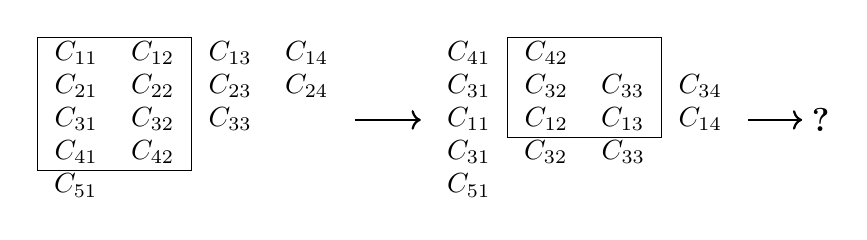
\begin{tikzpicture}
    \node (a) at (0, 0){
      \begin{tabular}{c c c c} \cline{1-2}
        \multicolumn{1}{|c}{$C_{11}$} & \multicolumn{1}{c|}{$C_{12}$} & $C_{13}$ & $C_{14}$ \\
        \multicolumn{1}{|c}{$C_{21}$} & \multicolumn{1}{c|}{$C_{22}$} & $C_{23}$ & $C_{24}$ \\
        \multicolumn{1}{|c}{$C_{31}$} & \multicolumn{1}{c|}{$C_{32}$} & $C_{33}$ &          \\
        \multicolumn{1}{|c}{$C_{41}$} & \multicolumn{1}{c|}{$C_{42}$} &                     \\ \cline{1-2}
        $C_{51}$                      &                               &
      \end{tabular}
    };
    \node (b) at (5, 0) {
      \begin{tabular}{c c c c} \cline{2-3}
        $C_{41}$ & \multicolumn{1}{|c}{$C_{42}$} & \multicolumn{1}{c|}{}         &          \\
        $C_{31}$ & \multicolumn{1}{|c}{$C_{32}$} & \multicolumn{1}{c|}{$C_{33}$} & $C_{34}$ \\
        $C_{11}$ & \multicolumn{1}{|c}{$C_{12}$} & \multicolumn{1}{c|}{$C_{13}$} & $C_{14}$ \\ \cline{2-3}
        $C_{31}$ & $C_{32}$                      & $C_{33}$                                 \\
        $C_{51}$ &
      \end{tabular}
    };
    \node (c) at (8, 0) {\large \bf{?}};
    \path[->, thick]
    (a.east) edge (b.west)
    (b.east) edge (c.west);
  \end{tikzpicture}
  \caption{Failure of unconditional pairs resampling}
  \label{fig:uncond-pairs-resample}
\end{figure}
Hence the only option is to carry out the resampling of each column pairs independently of the others, using the original data, and compute bootstrapped development factor and dispersion parameter estimates from these. The entire procedure is outlined in \cref{alg:pairs-mack}, and the results for the UK Motor dataset are given in \cref{tab:pairs-mack-res}.

\begin{algorithm}[!htb]
  \caption{Pairs bootstrap for \modelref{model:mack}}
  \label{alg:pairs-mack}
  \begin{algorithmic}
    \Require{Cumulative claims triangle $\mathcal{D}_I$, number of bootstrap samples $B$, parameter \textsc{conditional} specifying the resampling approach}
    \For{$b \gets 1, B$}
      \For{$j \gets 1, I - 1$}
        \vspace{5pt}
        \State $\{ (C^{(b)}_{i, j}, C^{(b)}_{i, j + 1}) \mid i = 1, \dots, I - j \} \gets$ \Call{resample}{$\{ (C_{i, j}, C_{i, j + 1}) \mid i = 1, \dots, I - j \}$}
        \vspace{5pt}
        \State $\widehat{f}^{(b)}_j \gets \sum_{i = 1}^{I - j} C^{(b)}_{i, j + 1} / \sum_{i = 1}^{I - j} C^{(b)}_{ij}$
        \vspace{5pt}
        \For{$i \gets 1, I - j$}
          \State $\displaystyle F^{(b)}_{i, j + 1} \gets C^{(b)}_{i, j + 1} / C^{(b)}_{ij}$
          \vspace{5pt}
        \EndFor
        \State $\displaystyle \widehat{\sigma}^{(b)}_j \gets \frac{1}{I-j}\sum_{i = 1}^{I-j} C^{(b)}_{ij}\left( F^{(b)}_{i, j + 1} - \widehat{f}^{(b)}_j \right)^2$
      \EndFor
    \EndFor
    \State \Return $\{ (\widehat{\bm{f}}^{(b)}, \widehat{\bm{\sigma}}^{(b)}) \mid b = 1, \dots, B \}$
  \end{algorithmic}
\end{algorithm}

\begin{table}[!htb]
  \centering
  \begin{subtable}{0.45\linewidth}
    \begin{tabularx}{\linewidth}{CCCCC}\toprule%
      $j$  & $\widehat{f}^B_j$ & $\widehat{\sigma}^B_j$ & $\widehat{R}_j^B$ & \resizebox{5em}{!}{$\widehat{\mathrm{MSEP}}(\widehat{R}_j)$} \\ \midrule
      \csvreader[
        head to column names,
      late after line =                                                                                                                    \\
      ]{%
        ../results/example/mack_pairs_param.csv
      }{}{%
      \idx & \devfacs          & \sigmas                & \reserve          & \prederror
      } \bottomrule%
    \end{tabularx}
    \subcaption{Parametric}
  \end{subtable}
  \hfill
  \begin{subtable}{0.45\linewidth}
    \begin{tabularx}{\linewidth}{CCCCC}\toprule%
      $j$  & $\widehat{f}^B_j$ & $\widehat{\sigma}^B_j$ & $\widehat{R}_j^B$ & \resizebox{5em}{!}{$\widehat{\mathrm{MSEP}}(\widehat{R}_j)$} \\ \midrule
      \csvreader[
        head to column names,
      late after line =                                                                                                                    \\
      ]{%
        ../results/example/mack_pairs_semiparam.csv
      }{}{%
      \idx & \devfacs          & \sigmas                & \reserve          & \prederror
      } \bottomrule%
    \end{tabularx}
    \subcaption{Semiparametric}
  \end{subtable}
  \caption{Pairs bootstrap results}
  \label{tab:pairs-mack-res}
\end{table}

Finally, we discuss the parametric bootstrap, in which we simulate directly from the fitted model. Based on \cref{eq:time-series-model}, we might be tempted to simply substitute $\mathcal{N}(0, 1)$-distributed draws from a random number generator for the residuals in \cref{alg:cond-semiparam-mack,alg:uncond-semiparam-mack}. The problem with this approach, is that it doesn't extend easily to other distributions, because it is not possible, in general, to write these as the sum of a mean and a scaled error term. A better idea, then, is to generate bootstrap responses directly from the fitted distribution. Depending on whether the conditional or the unconditional scheme is used, this will either depend on the original triangle observations or the ones generated at the previous step. \Modelref{model:mack} is then refitted to the bootstrapped triangle in order to obtain $\widehat{\bm{f}}^{(b)}$ and $\widehat{\bm{\sigma}}^{(b)}$. The algorithms and results are given in \Cref{alg:cond-param-mack,alg:uncond-param-mack,tab:param-mack-res}.

\begin{figure}[p]
  \begin{algorithm}[H]
    \caption{Conditional parametric bootstrap for \modelref{model:mack}}
    \label{alg:cond-param-mack}
    \begin{algorithmic}
      \Require{Cumulative claims triangle $\mathcal{D}_I$, number of bootstrap samples $B$}
      \State $(\bm{\widehat{f}}, \bm{\widehat{\sigma}}) \gets$ \Call{fit}{$\mathcal{D}_I$}
      \For{$b \gets 1, B$}
        \For{$j \gets 1, I - 1$}
          \For{$i \gets 1, I - j$}
            \State $C^{(b)}_{i, j + 1} \gets$ \Call{sample}{$ \, \mathcal{N}(\widehat{f}_j C_{ij}, \widehat{\sigma}^2_j C_{ij}) \, $}
            \State $\displaystyle F^{(b)}_{i, j + 1} \gets C^{(b)}_{i, j + 1} / C_{ij}$
          \EndFor
          \State $\widehat{f}^{(b)}_j \gets \sum_{i = 1}^{I - j} C^{(b)}_{i, j + 1} / \sum_{i = 1}^{I - j} C_{ij}$
          \If{$j < I - 1$}
            \State $\displaystyle \widehat{\sigma}^{(b)}_j \gets \frac{1}{I - j - 1}\sum_{i = 1}^{I - j} C_{ij} \left( F^{(b)}_{i, j + 1} - \widehat{f}^{(b)}_j \right)^2$
          \Else
            \State $\widehat{\sigma}^{(b)}_{I - 1} \gets \sqrt{\min{ \left \{ \displaystyle \frac{(\widehat{\sigma}^{(b)}_{I - 2})^4}{(\widehat{\sigma}^{(b)}_{I - 3})^2}, (\widehat{\sigma}^{(b)}_{I - 2})^2, (\widehat{\sigma}^{(b)}_{I - 3})^2 \right \} }}$
          \EndIf
        \EndFor
      \EndFor
      \State \Return $\{ (\widehat{\bm{f}}^{(b)}, \widehat{\bm{\sigma}}^{(b)}) \mid b = 1, \dots, B \}$
    \end{algorithmic}
  \end{algorithm}
  %
  \begin{algorithm}[H]
    \caption{Unconditional parametric bootstrap for \modelref{model:mack}}
    \label{alg:uncond-param-mack}
    \begin{algorithmic}
      \Require{Cumulative claims triangle $\mathcal{D}_I$, number of bootstrap samples $B$}
      \State $(\{ r_{ij} \mid i + j \leq I + 1 \}, \bm{\widehat{f}}, \bm{\widehat{\sigma}}) \gets$ \Call{fit}{$\mathcal{D}_I$}
      \For{$b \gets 1, B$}
        \For{$i \gets 1, I$}
          \State $C^{(b)}_{i1} \gets C_{i1}$
        \EndFor
        \For{$j \gets 1, I - 1$}
          \For{$i \gets 1, I - j$}
            \State $C^{(b)}_{i, j + 1} \gets$ \Call{sample}{$ \, \mathcal{N}(\widehat{f}_j C^{(b)}_{ij}, \widehat{\sigma}^2_j C^{(b)}_{ij}) \, $}
            \State $\displaystyle F^{(b)}_{i, j + 1} \gets C^{(b)}_{i, j + 1} / C^{(b)}_{ij}$
          \EndFor
          \State $\widehat{f}^{(b)}_j \gets \sum_{i = 1}^{I - j} C^{(b)}_{i, j + 1} / \sum_{i = 1}^{I - j} C^{(b)}_{ij}$
          \If{$j < I - 1$}
            \State $\displaystyle \widehat{\sigma}^{(b)}_j \gets \frac{1}{I - j - 1}\sum_{i = 1}^{I - j} C^{(b)}_{ij} \left( F^{(b)}_{i, j + 1} - \widehat{f}^{(b)}_j \right)^2$
          \Else
            \State $\widehat{\sigma}^{(b)}_{I - 1} \gets \sqrt{\min{ \left \{ \displaystyle \frac{(\widehat{\sigma}^{(b)}_{I - 2})^4}{(\widehat{\sigma}^{(b)}_{I - 3})^2}, (\widehat{\sigma}^{(b)}_{I - 2})^2, (\widehat{\sigma}^{(b)}_{I - 3})^2 \right \} }}$
          \EndIf
        \EndFor
      \EndFor
      \State \Return $\{ (\widehat{\bm{f}}^{(b)}, \widehat{\bm{\sigma}}^{(b)}) \mid b = 1, \dots, B \}$
    \end{algorithmic}
  \end{algorithm}
\end{figure}

\begin{table}[!htb]
  \centering
  \begin{subtable}{0.45\textwidth}
    \begin{tabular}{ m{1em} m{2em} m{2em} m{3.5em} m{4em} }\toprule%
      $j$  & $\widehat{f}^B_j$ & $\widehat{\sigma}^B_j$ & $\widehat{R}_j^B$ & \resizebox{4em}{!}{$\widehat{\mathrm{MSEP}}(\widehat{R}_j)$} \\ \midrule
      \csvreader[
        head to column names,
      late after line =                                                                                                                    \\
      ]{%
        ../results/example/mack_param_cond_norm.csv
      }{}{%
      \idx & \devfacs          & \sigmas                & \reserve          & \prederror
      } \bottomrule
    \end{tabular}
    \subcaption{Conditional}
  \end{subtable}
  \begin{subtable}{0.45\textwidth}
    \begin{tabular}{ m{1em} m{2em} m{2em} m{3.5em} m{4em} }\toprule%
      $j$  & $\widehat{f}^B_j$ & $\widehat{\sigma}^B_j$ & $\widehat{R}_j^B$ & \resizebox{4em}{!}{$\widehat{\mathrm{MSEP}}(\widehat{R}_j)$} \\ \midrule
      \csvreader[
        head to column names,
      late after line =                                                                                                                    \\
      ]{%
        ../results/example/mack_param_uncond_norm.csv
      }{}{%
      \idx & \devfacs          & \sigmas                & \reserve          & \prederror
      } \bottomrule
    \end{tabular}
    \subcaption{Unconditional}
  \end{subtable}
  \caption{Parametric bootstrap results for normal distribution}
  \label{tab:param-mack-res-norm}
\end{table}

\begin{table}[!htb]
  \centering
  \begin{subtable}{0.45\textwidth}
    \begin{tabular}{ m{1em} m{2em} m{2em} m{3.5em} m{4em} }\toprule%
      $j$  & $\widehat{f}^B_j$ & $\widehat{\sigma}^B_j$ & $\widehat{R}_j^B$ & \resizebox{4em}{!}{$\widehat{\mathrm{MSEP}}(\widehat{R}_j)$} \\ \midrule
      \csvreader[
        head to column names,
      late after line =                                                                                                                    \\
      ]{%
        ../results/example/mack_param_cond_gamma.csv
      }{}{%
      \idx & \devfacs          & \sigmas                & \reserve          & \prederror
      } \bottomrule
    \end{tabular}
    \subcaption{Conditional}
  \end{subtable}
  \begin{subtable}{0.45\textwidth}
    \begin{tabular}{ m{1em} m{2em} m{2em} m{3.5em} m{4em} }\toprule%
      $j$  & $\widehat{f}^B_j$ & $\widehat{\sigma}^B_j$ & $\widehat{R}_j^B$ & \resizebox{4em}{!}{$\widehat{\mathrm{MSEP}}(\widehat{R}_j)$} \\ \midrule
      \csvreader[
        head to column names,
      late after line =                                                                                                                    \\
      ]{%
        ../results/example/mack_param_uncond_gamma.csv
      }{}{%
      \idx & \devfacs          & \sigmas                & \reserve          & \prederror
      } \bottomrule
    \end{tabular}
    \subcaption{Unconditional}
  \end{subtable}
  \caption{Parametric bootstrap results for gamma distribution}
  \label{tab:param-mack-res-gamma}
\end{table}

\section{Incorporating the process error} \label{sec:mack-proc}

We end this chapter by discussing how the process error can be incorporated into these bootstrap procedures. As described in \cref{sec:boot-proc}, our aim is to obtain a predictive distribution of the reserve which incorporates both parameter and process error. Following the procedure outlined there, we can achieve this by simulating the lower triangle $\mathcal{D}^{\mathsf{c}}_I = \{ C_{ij} \mid i + j > I + 1 \}$, giving us pseudo-realisations of the future claim amounts. This will then in turn yield bootstrap replicates
\begin{equation}
  R^{(b)} \coloneqq \sum_{i = 2}^I (C^{(b)}_{iI} - C_{i, I + 1 - i})
\end{equation}
for the reserve. The method proposed in \cite{england:dist} is based on \eqref{eq:time-series-model}: starting from the antidiagonal of $\mathcal{D}_I$, we recursively sample
\begin{equation} \label{eq:normal-sampling}
  C^{(b)}_{i, j + 1} \sim \mathcal{N}(\widehat{f}^{(b)}_j \, C^{(b)}_{ij}, \widehat{\sigma}^{(b)}_j \, C_{ij}) \,,
\end{equation}
\newgeometry{bottom=0.1cm}
\noindent until the final development year $I$ is reached. As noted in \cref{sec:mack-boot} when discussing the semiparametric bootstrap, however, this approach makes it possible to draw negative samples, which is problematic. The remedies available to us here depend on the type of bootstrap employed. It is possible to avoid this difficulty with the semiparametric bootstrap by using the residuals from \cref{eq:log-normal-resids}, which are based on the shifted log-normal distribution. For the parametric bootstrap, we can follow the suggestion from \cite{england:dist}, discussed in the previous section, and use \cref{eq:gamma-sim} to simulate future claim amounts. The solution adopted for the pairs bootstrap will depend on which of the two other variants is used in the simulation step.

In the synthetic example we gave in \cref{sec:boot-proc}, not much difference could be discerned between the fitted and predictive distributions. This stands in stark contrast to \cref{fig:fit-pred-pairs,fig:fit-pred-semiparam,fig:fit-pred-param}, which compare these for the reserve under different bootstrap configurations. We can clearly see that fitted distribution severely underestimates the uncertainty of the reserve in all cases.

\begin{figure}[!htb]
  \begin{subfigure}{0.45 \textwidth}
    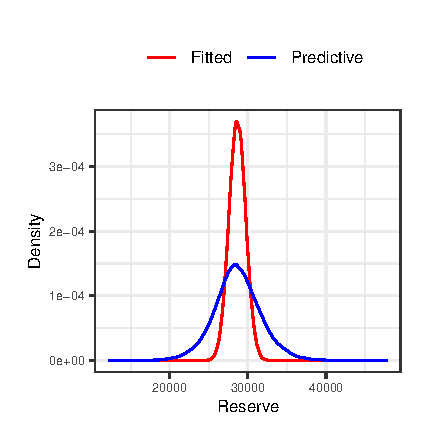
\includegraphics{mack_pairs_param}
    \subcaption{Parametric}
  \end{subfigure}
  \begin{subfigure}{0.45 \textwidth}
    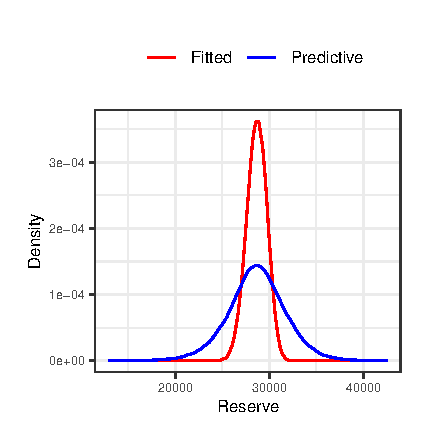
\includegraphics{mack_pairs_semiparam}
    \subcaption{Semiparametric}
  \end{subfigure}
  \caption{Comparison of the fitted and predictive distribution from the pairs bootstrap for different methods in the prediction step}
  \label{fig:fit-pred-pairs}
\end{figure}

\begin{figure}[!htb]
  \begin{subfigure}{0.45 \textwidth}
    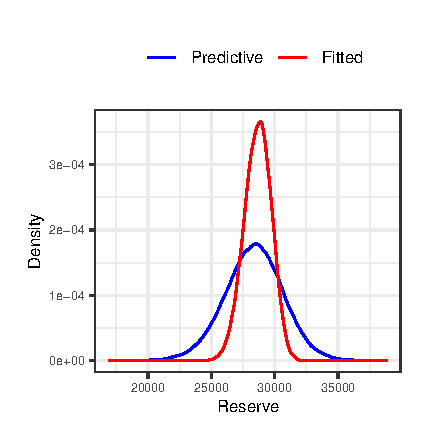
\includegraphics{mack_semiparam_cond_standard}
    \subcaption{Conditional}
  \end{subfigure}
  \begin{subfigure}{0.45 \textwidth}
    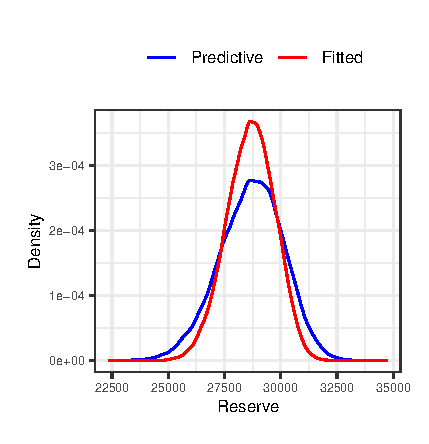
\includegraphics{mack_semiparam_uncond_standard}
    \subcaption{Unconditional}
  \end{subfigure}
  \caption{Comparison of the fitted and predictive distribution for the semiparametric bootstrap}
  \label{fig:fit-pred-semiparam-standard}
\end{figure}

\begin{figure}[!htb]
  \begin{subfigure}{0.45 \textwidth}
    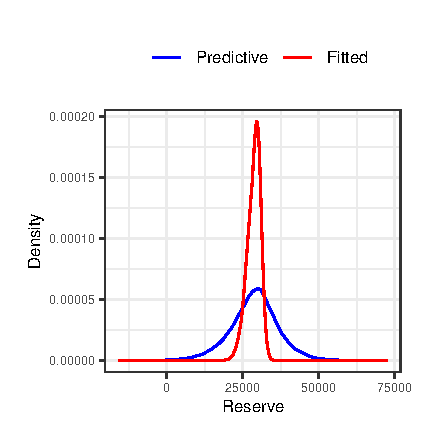
\includegraphics{mack_semiparam_cond_student}
    \subcaption{Conditional}
  \end{subfigure}
  \begin{subfigure}{0.45 \textwidth}
    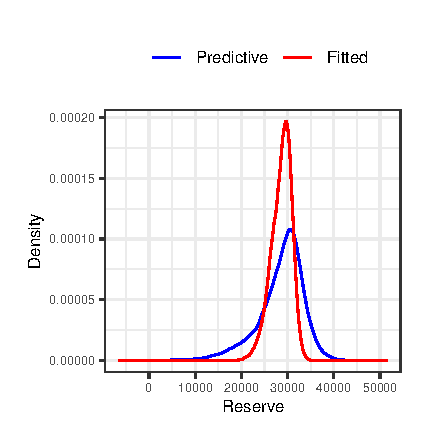
\includegraphics{mack_semiparam_uncond_student}
    \subcaption{Unconditional}
  \end{subfigure}
  \caption{Comparison of the fitted and predictive distribution for the semiparametric bootstrap}
  \label{fig:fit-pred-semiparam-student}
\end{figure}

\begin{figure}[!htb]
  \begin{subfigure}{0.45 \textwidth}
    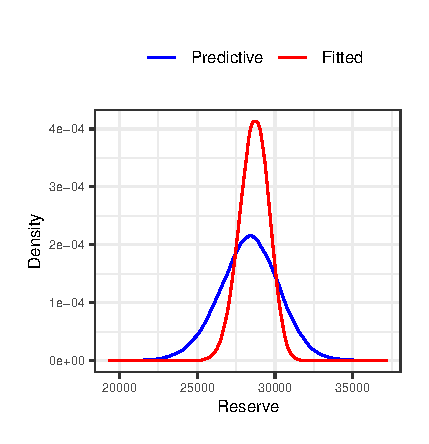
\includegraphics{mack_semiparam_cond_log_normal}
    \subcaption{Conditional}
  \end{subfigure}
  \begin{subfigure}{0.45 \textwidth}
    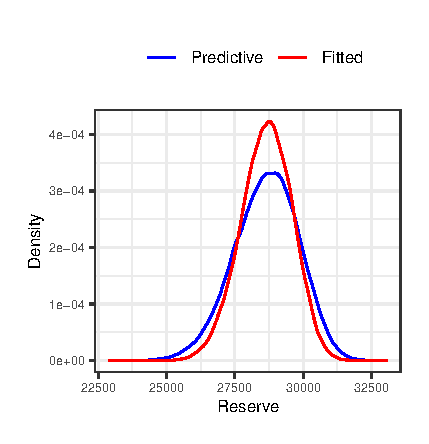
\includegraphics{mack_semiparam_uncond_log_normal}
    \subcaption{Unconditional}
  \end{subfigure}
  \caption{Comparison of the fitted and predictive distribution for the semiparametric bootstrap}
  \label{fig:fit-pred-semiparam-lognromal}
\end{figure}

\restoregeometry

\begin{landscape}
  \begin{figure}
    \begin{subfigure}{\linewidth}
      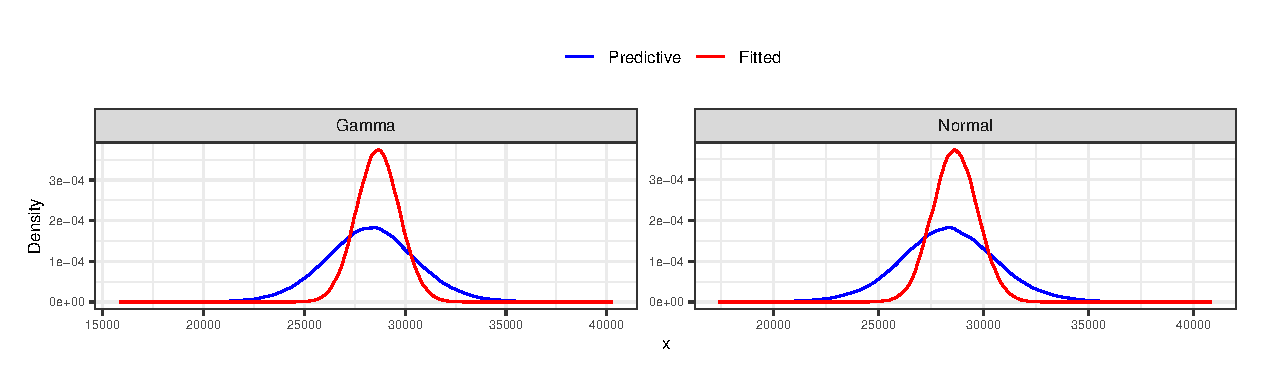
\includegraphics{mack_param_cond}
      \subcaption{Conditional}
    \end{subfigure}
    \begin{subfigure}{\linewidth}
      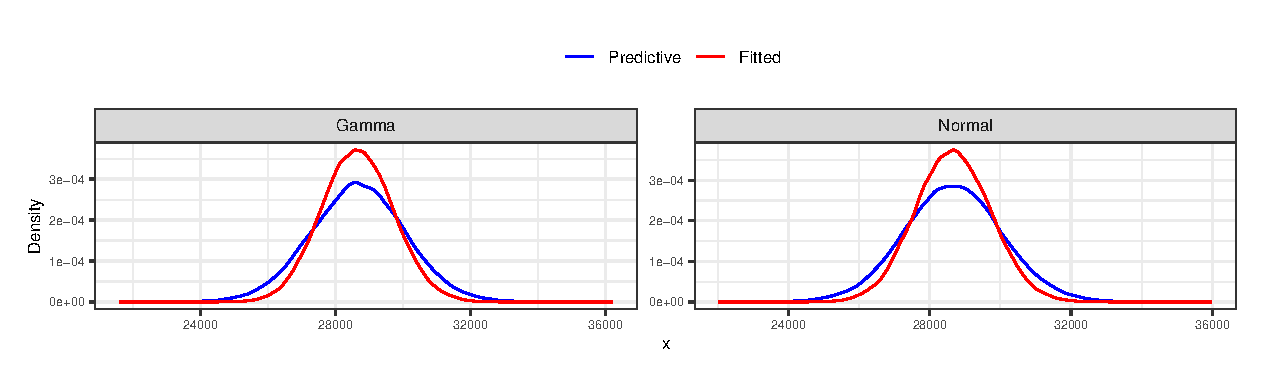
\includegraphics{mack_param_uncond}
      \subcaption{Unconditional}
    \end{subfigure}
    \caption{Comparison of the fitted and predictive distribution for the parametric bootstrap}
    \label{fig:fit-pred-param}
  \end{figure}
\end{landscape}

\chapter{Overdispersed Poisson GLM} \label{chapter:poisson}

The overdispersed Poisson model (ODP), proposed by Renshaw and Verrall in \cite{renshaw}, belongs to the family of so-called \emph{generalised linear models} (GLM). In contrast to \modelref{model:mack}, it describes the incremental claims $X_{ij}$, and is non-recursive: the diffferent observations in the triangle are modelled independently from each other. To ease the exposition, we will only state the assumptions for the ordinary Poisson model (i.e. without overdispersion) at this point; after this concept has been introduced in \cref{subsec:quasi}, we will then adjust the model accordingly.

\begin{model}[Poisson GLM] \leavevmode \label{model:poisson}
  \begin{enumerate}[label=\bf{\textup{(}Pois\arabic*\textup{)}},ref=\textup{(}Pois\arabic*\textup{)}, wide]
    \item \label{assump:poisson1}
          The incremental claims are independent from each other.
    \item \label{assump:poisson2}
          There exist parameters $c$, $a_1, \dots, a_I$ and $b_1, \dots, b_I$ such that
          \begin{equation} \label{eq:linear-predictor-poisson}
            \log(\expect{X_{ij}}) = c + a_i + b_j \,,
          \end{equation}
          with $a_1 = b_1 = 0$.
    \item \label{assump:poisson3}
          The incremental claims follow a Poisson distribution with $\mu_{ij} = \expect{X_{ij}}$:
          \begin{equation}
            X_{ij} \sim \mathrm{Pois}(e^{c + a_i + b_j}) \,.
          \end{equation}
  \end{enumerate}
\end{model}

The condition $a_1 = b_1 = 0$ is necessary to obtain an identifiable model. Without it, we could obtainm, from any set of parameters $c, a_1, \dots, a_I, b_1, \dots, b_I$ satisfying the assumptions, an infinite number of alternatives $c + a_0 + b_0, a_1 - a_0, \dots, a_I - a_0, b_1 - b_0, \dots, b_I - b_0$ for $a_0, b_0 \in \mathbb{R}$. We therefore have two superfluous degrees of freedom, which can be eliminated by imposing the same number of conditions on the parameters.

By defining $\xi_i \coloneqq e^{c + a_i}$ and $\gamma_j \coloneqq e^{b_j}$, we can obtain a different parametrisation of the model which has a multiplicative structure for the mean, i.e.
\begin{equation}
  \expect{X_{ij}} = \xi_i \gamma_j \,.
\end{equation}
This is sometimes preferred to the additive one for reasons of interpretability. Indeed, it is clear that the multiplicative form has one fewer degree of freedom than the linear one, and if we remove it by imposing the constraint
\begin{equation}
  \sum_{j = 1}^I \gamma_j = 1
\end{equation}
then we can view the $\xi_i$ as expected ultimate claim amounts, and the $\gamma_j$ as the expected development pattern.

As mentioned in the introduction, stochastic claims reserving models have to reproduce the chain ladder point predictions in order to be acceptable to practitioners. While less obvious than for \modelref{model:mack}, it can be shown that \modelref{model:poisson} also satisfies this requirement (see \cite[Lemma 2.16]{wuthrich:stochastic-reserving}), as we shall see in \cref{tab:pois-bench}.

\section{Generalised linear models} \label{sec:glm}

GLMs were first conceived by Nelder and Wedderburn in \cite{nelder} as a way of unifying the many disparate generalisations of linear regression with Gaussian errors which were then in existence. These sought to extend the classical model by allowing the use of different functional forms for the conditional mean and different distributions for the response, thus making it suited to modelling counts data (Poisson regression) or the probability of binary events (logistic regression), among others. For a set of covariates $X_1, \dots, X_p$ and a response variable $Y$, a GLM consists of three parts:
\begin{enumerate}
  \item The \emph{random component}, a distribution for response $Y$ belonging to the so-called \emph{exponential dispersion model} family (EDM), which consists of all probability distributions whose density (with respect either to the Lebesgue or counting measure) has the form
        \begin{equation} \label{eq:exp-disp-fam}
          p(y \mid \theta, \phi) = \exp \left \{ \frac{y \theta - b(\theta)}{a(\phi)} + c(y, \phi) \right \} \,,
        \end{equation}
        where $a$, $b$ and $c$ are known functions, and $b$ is at least twice differentiable. We call $\theta$ the \emph{canonical parameter} of the distribution and $\phi$ the \emph{dispersion parameter}.
  \item The \emph{systematic component}, a predictor $\eta \coloneqq \bm{\mathrm{x}}^T \bm{\beta}$ which is a linear function of the covariates.
  \item A monotonic differentiable link function $g: \mathbb{R} \rightarrow \mathbb{R}$ giving the relation between the conditional expectation and the linear predictor,
        \begin{equation}
          \mu \coloneqq \condexpp{Y}{X_1, \dots, X_p} = g^{-1}(\eta) \,.
        \end{equation}
\end{enumerate}
The Gaussian distribution $\mathcal{N}(\mu, \sigma^2)$ can be seen to belong to the EDM family by rewriting its density as
\begin{align}
  \frac{1}{\sqrt{2 \pi} \sigma} \exp \left \{ -\frac{1}{2} \left( \frac{y - \mu}{\sigma} \right)^2\right \} & = \exp \left \{ -\frac{y^2}{2 \sigma^2} + \frac{y \mu}{\sigma^2} - \frac{\mu^2}{2 \sigma^2} - \log(\sqrt{2 \pi} \sigma) \right \} \\
                                                                                                            & = \exp \left \{ \frac{y \mu - \mu^2 / 2}{\sigma^2} - \frac{y^2}{2 \sigma^2} - \log(\sqrt{2 \pi} \sigma) \right \} \,,
\end{align}
which is of the form \cref{eq:exp-disp-fam} with $\theta = \mu$, $b(\theta) = \frac{\theta^2}{2}$, $\phi = \sigma^2$, $a(\phi) = \phi$ and $c(y, \sigma) = -\frac{y^2}{2 \sigma^2} - \log(\sqrt{2 \pi} \sigma)$. Thus, the familiar normal linear model can be obtained from the GLM framework with response distribution $\mathcal{N}(\mu, \sigma^2)$ and identity link $g(\mu) = \mu$.

\subsection{Estimation}

The EDM family has a number of properties which greatly facilitate the computations involved in estimation. Recall from likelihood theory that $l(\theta \mid y, \phi) \coloneqq \log p(y \mid \theta, \phi)$ satisfies
\begin{equation} \label{eq:exp-var-likelihood}
  \expect{\frac{\partial l(\theta \mid Y)}{\partial \theta}} = 0 \,, \qquad \var{\frac{\partial l(\theta \mid Y)}{\partial \theta}} = -\expect{\frac{\partial^2 l(\theta \mid Y)}{\theta^2}} \,,
\end{equation}
where $\frac{\partial l(\theta \mid Y)}{\partial \theta}$ is known as the \emph{score function}. Using \cref{eq:exp-disp-fam}, we then find that
\begin{equation}
  \expect{\frac{Y - b'(\theta)}{a(\phi)}} = 0 \,, \qquad \var{\frac{Y - b'(\theta)}{a(\phi)}} = -\expect{\frac{-b''(\theta)}{a(\phi)}} \,,
\end{equation}
from which we obtain the elegant relations
\begin{equation}
  \mu = b'(\theta) \,, \qquad \var{Y} = a(\phi) b''(\theta) \,.
\end{equation}
Observe that this implies that $\frac{d \mu}{d \theta} = b''(\theta) > 0$ (because the variance is always positive), which means that $\theta \mapsto \mu(\theta)$ is one-to-one and therefore invertible. In particular, we can always write the likelihood as function of the mean. The function $V(\mu) \coloneqq b''((b')^{-1}(\mu))$ is called the \emph{variance function} and determines how the scale of the response varies as a function of its mean.

Special care has to be taken with the parameter $\phi$, as it occupies a rather awkward position in GLM theory. The trouble is that we want to incorporate two-parameter distributions, such as the normal and gamma distribution, into the GLM framework which can fundamentally only handle a single parameter gracefully (the more flexible framework of \emph{vector GLMs} is an attempt to remedy this; see \cite[Chapter 2]{yee} for a general discussion). The dispersion is therefore regelated to the role of nuisance parameter and subjected to severe (and often unrealistic) constraints. Basically, we $\phi$ to be the constant as a function of the covariates, but this would preclude certain special cases such as binomial regression with a different number of trials for each observation in the sample. To take this into account, we allow the function $a$ in the denominator of \cref{eq:exp-disp-fam} to vary across different sample responses as $a_i(\phi) = \phi / w_i$, where $w_i$ is a known weight. Not a very elegant solution, perhaps, but one which is foisted upon us by the limitations of the theory. The parameter $\phi$ itself is then considered as known, and estimated outside of the GLM framework, most commonly using the Pearson statistic
\begin{equation}
  \widehat{\phi} \coloneqq \frac{1}{n - p} \sum_{i = 1}^N \frac{(Y_i - \widehat{\mu_i})^2}{V(\widehat{\mu_i})} \,.
\end{equation}

Given a sample $(\bm{\mathrm{x_1}}, Y_1), \dots, (\bm{\mathrm{x_N}}, Y_N)$, the standard way to fit a GLM is by means of maximum likelihood estimation (MLE). The joint log-likelihood of the sample is given by
\begin{equation} \label{eq:joint-log-likelihood}
  l(\bm{\beta} \mid \mathbf{y}, \phi) = \sum_{i = 1}^N \frac{y_i \theta_i - b(\theta_i)}{a_i(\phi)} + c(y_i, \phi) \,,
\end{equation}
which we must differentiate with respect to $\beta_j$ to obtain the likelihood equations. An application of the chain rule gives us
\begin{align}
  \frac{\partial l(\bm{\beta} \mid \mathbf{y}, \phi)}{\partial \beta_j} & = \sum_{i = 1}^N \frac{\partial l(\bm{\beta} \mid y_i, \phi)}{\partial \theta_i} \frac{\partial \theta_i}{\partial \mu_i} \pdv{\mu_i}{\eta_i} \frac{\partial \eta_i}{\partial \beta_j} \\
                                                                        & = \sum_{i = 1}^N \frac{y_i - b'_i(\theta)}{a_i(\phi)} \frac{1}{b_i''(\theta_i)} \pdv{\mu_i}{\eta_i} x_{ij}                                                                             \\
                                                                        & = \sum_{i = 1}^N \frac{y_i - \mu_i}{\var{Y_i}} \pdv{\mu_i}{\eta_i} x_{ij} \,, \label{eq:grad-likelihood}
\end{align}
and setting this equal to $0$ yields a system of $p$ (usually nonlinear) equations. It is generally impossible to solve these analytically, and so we must resort to numerical methods. In particular, we use a modified version of the Newton-Raphson algorithm known as \emph{Fisher scoring}, which replaces the negative Hessian of the log-likelihood, called the \emph{observed information}, by its expectation
\begin{equation}
  \mathcal{I}_{jk} \coloneqq \expect{-\frac{\partial^2 l(\bm{\beta} \mid \mathbf{y}, \phi)}{\partial \beta_j \partial \beta_k}} \,,
\end{equation}
which is known as the \emph{Fisher information matrix}. Thus, starting from an initial guess $\bm{\widehat{\beta}}^{(0)}$ for the parameters, we compute a successive approximations via
\begin{equation} \label{eq:fisher-scoring}
  \bm{\widehat{\beta}}^{(k + 1)} = \bm{\widehat{\beta}}^{(k)} + \mathcal{I}(\bm{\widehat{\beta}}^{(k)})^{-1} \nabla l(\bm{\widehat{\beta}}^{(k)} \mid \mathbf{y}, \phi) \,.
\end{equation}
Similarly to \cref{eq:exp-var-likelihood}, it can be shown that
\begin{equation}
  \expect{\pdv{l(\bm{\beta} \mid \mathbf{y}, \phi)}{\bm{\beta}, \bm{\beta}^T}} = -\var{\nabla l(\bm{\beta} \mid \mathbf{y}, \phi) \nabla l(\bm{\beta} \mid \mathbf{y}, \phi)^T} < 0 \,,
\end{equation}
from which we also see that the log-likelihood is concave, and will therefore have a global maximum. Using the fact that the $Y_i$ are independent, so that $\expect{(Y_i - \mu_i)(Y_l - \mu_l)} = 0$ for $i \neq l$, we then obtain
\begin{align}
  I_{jk} & = \expect{\left( \sum_{i = 1}^N \frac{Y_i - \mu_i}{\var{Y_i}} \pdv{\mu_i}{\eta_i} x_{ij}\right) \left( \sum_{l = 1}^N \frac{Y_l - \mu_l}{\var{Y_l}} \frac{\partial \mu_l}{\partial \eta_l} x_{lk} \right)} \\
         & = \sum_{i = 1}^N \left( \pdv{\mu_i}{\eta_i} \right)^2 \frac{\expect{(Y_i - \mu_i)^2}}{\var{Y_i}^2} x_{ij} x_{ik}                                                                                           \\
         & = \sum_{i = 1}^N \left( \pdv{\mu_i}{\eta_i} \right)^2 \frac{x_{ij} x_{ik}}{\var{Y_i}}                                                                                                                      \\
         & = \bm{\mathrm{x}_j}^T \mathbf{W} \bm{\mathrm{x}_k} \label{eq:information-comps}
\end{align}
where $\mathbf{W}^{(k)}$ is a diagonal matrix with
\begin{equation} \label{eq:irwls-weight-mat}
  \mathbf{W}^{(k)}_{ii} = \frac{1}{\var{Y_i}} \pdv{\mu_i}{\eta_i}_{\bm{\widehat{\beta}}^{(k)}}^2 \,.
\end{equation}
Hence we have $\mathcal{I}(\bm{\widehat{\beta}}^{(k)}) = \mathbf{X}^T \mathbf{W}^{(k)} \mathbf{X}$ and we see from \cref{eq:grad-likelihood} that
\begin{equation} \label{eq:irwls-grad}
  \nabla l(\bm{\beta} \mid \mathbf{y}, \phi) = \mathbf{X}^T \mathbf{W} \mathbf{\tilde{z}}
\end{equation}
with $\mathbf{\tilde{z}}_i = (y_i - \mu_i) \left( \pdv{\eta_i}{\mu_i} \right)$. Multiplying both sides of \ref{eq:fisher-scoring} by $\mathcal{I}(\bm{\beta}^{(k)})$ and using \cref{eq:irwls-weight-mat,eq:irwls-grad,eq:information-comps}, we finally obtain
\begin{align} \label{eq:irwls-iter}
  \mathbf{X}^T \mathbf{W}^{(k)} \mathbf{X} \bm{\widehat{\beta}}^{(k + 1)} =  \mathbf{X}^T \mathbf{W}^{(k)} \mathbf{z}
\end{align}
with $\mathbf{z} = \mathbf{X} \bm{\widehat{\beta}}^{(k)} + \mathbf{\tilde{z}}$ and all quantities evaluated at the current estimate $\bm{\beta}^{(k)}$ of the parameter vector. In other words, the Fisher scoring is equivalent to a series of weighted least squares problems, where the new parameter estimates are obtained by regressing the vector $\mathbf{z}$ on the original covariates $\bm{\mathrm{x}_1}, \dots, \bm{\mathrm{x}_N}$ using weight matrix $\mathbf{W}$, and $\mathbf{z}$ and $\mathbf{W}$ are determined by the current estimate $\bm{\beta}^{(k)}$---hence why the algorithm is called \emph{iteratively reweighted least squares} (IRWLS).

This procedure can be specialised to the particular case of \modelref{model:poisson} in the following way. First, in order to obtain the matrix-vector form used above, we must flatten the tabular response (using, for example, the colexicographical ordering $(i, j) \mapsto j I + i$, i.e.\ column-major order). This gives us a triangle in long format, as illustrated in \cref{tab:uk-motor-long} for the incremental form of the UK Motor dataset from \textcite{christofides}.
\begin{table}[!htb]
  \centering
  \begin{tabularx}{0.3 \linewidth}{CCC}\toprule%
    origin  & dev  & value  \\ \midrule
    \csvreader[
    late after line =       \\
    ]{%
      ../results/example/UKMotor_long.csv
    }{origin=\Origin, dev=\Dev, value=\Value}{%
    \Origin & \Dev & \Value
    }\bottomrule%
  \end{tabularx}
  \caption{UK Motor incremental claims triangle in long format}
  \label{tab:uk-motor-long}
\end{table}
If we define the parameter vector
\begin{equation}
  \bm{\beta} \coloneqq \begin{bmatrix} c & a_2 & \cdots & a_I & b_2 & \cdots & b_I \end{bmatrix}^T \,,
\end{equation}
then \cref{eq:linear-predictor-poisson} can be rewritten as
\begin{equation} \label{eq:poisson-covariates}
  \log(\mu_{ij}) = c + a_i + b_j = (\bm{\mathrm{e}_1} + \bm{\mathrm{e}_i} + \bm{\mathrm{e}_{I + j - 1}})^T \bm{\beta}
\end{equation}
where $\bm{\mathrm{e}_k}$ denotes the $k$th standard basis vector in $\mathbb{R}^{(2I - 1)}$. Hence we see that the covariates are binary vectors of length $2I - 1$, with the position of the nonzero entries determined by the indices of the observation in the triangle, forming the rows of a very sparse design matrix. As \modelref{model:poisson} uses the log link, we have $\mu_{ij} = e^{\eta_{ij}}$ and
\begin{equation}
  \frac{\partial \mu_{ij}}{\partial \eta_{ij}} = e^{\eta_{ij}} \,,
\end{equation}
from which, using \cref{eq:irwls-weight-mat}, we finally obtain
\begin{equation}
  \mathbf{W}_{ii} = \frac{1}{e^{\eta_{ij}}} (e^{\eta_{ij}})^2 = e^{\eta_{ij}} \,,
\end{equation}
giving us all the components of the IRWLS algorithm. \cref{fig:glm-mat-eq} shows in matrix form.

\begin{figure}
  \centering
  \large
  \begin{displaymath}
    \begin{split}
      &\underbrace{
        \begin{bmatrix}
          1      & 0      & 0      & \dots & 0      \\
          1      & 1      & 0      & \dots & 0      \\
          \vdots & \vdots & \vdots &       & \vdots \\
          1      & 0      & 0      & \dots & 1      \\
        \end{bmatrix}
      }_{\mathbf{X}^T}
      \underbrace{
        \begin{bmatrix}
          e^{\widehat{c}^{(k)}} &                                             &        &                                                                     \\
                                & e^{\widehat{c}^{(k)} + \widehat{a}^{(k)}_1} &        &                                                                   & \\
                                &                                             & \ddots &                                                                     \\
                                &                                             &        & e^{\widehat{c}^{(k)} + \widehat{a}^{(k)}_I + \widehat{b}^{(k)}_I}   \\
        \end{bmatrix}
      }_{\mathbf{W}^{(k)}}
      \underbrace{
        \begin{bmatrix}
          1      & 1      & 1      & \dots & 1      \\
          0      & 1      & 0      & \dots & 0      \\
          \vdots & \vdots & \vdots &       & \vdots \\
          0      & 0      & 0      & \dots & 1      \\
        \end{bmatrix}
      }_{\mathbf{X}}
      \underbrace{
        \begin{bmatrix}
          c \\ a^{(b)}_2 \\ \vdots \\ a^{(b)}_I \\ b^{(b)}_2 \\ \vdots \\ b^{(b)}_I
        \end{bmatrix}
      }_{\bm{\widehat{\beta}}^{(b)}} \\
      &=%
      \underbrace{
        \begin{bmatrix}
          1      & 0      & 0      & \dots & 0      \\
          1      & 1      & 0      & \dots & 0      \\
          \vdots & \vdots & \vdots &       & \vdots \\
          1      & 0      & 0      & \dots & 1      \\
        \end{bmatrix}
      }_{\mathbf{X}^T}
      \underbrace{
        \begin{bmatrix}
          e^{c} &             &        &                     \\
                & e^{c + a_1} &        &                   & \\
                &             & \ddots &                     \\
                &             &        & e^{c + a_I + b_I}   \\
        \end{bmatrix}
      }_{\mathbf{W}^{(k)}}
      \mathbf{z}
    \end{split}
  \end{displaymath}
  \caption{IRWLS equation for Poisson GLM in matrix form}
  \label{fig:glm-mat-eq}
\end{figure}

\subsection{Quasi-likelihood methods} \label{subsec:quasi}

We have assumed up to this point that a GLM requires us to specify an exact distribution for the response variable. In many practical situations, however, this is either infeasible or leads to unrealistic models. An example which is particularly common with count data is a phenomenon known as \emph{overdispersion}, where the variability of the data is greater than would be suggested by e.g.\ the Poisson or binomial distribution. Recall that the variance of a $\mathrm{Pois}(\lambda)$ distribution is $\lambda$, and that of a $B(n, p)$ distribution is $np(1 - p)$; in both cases, it is fully determined by the mean, and we have no degree of freedom with which to adjust it in order to obtain a better fit to the data, as would be the case with the normal distribution, for example.

To remedy this, an extension can be made to the GLM framework, which only relies on the specification of a relation between mean and variance. Recall from above that the MLE works by setting the score equal to $0$. If we write the likelihood in terms of $\bm{\mu}$, this will have components
\begin{equation} \label{eq:lhood-mean-param}
  \frac{\partial l(\bm{\mu} \mid \mathbf{y}, \phi)}{\partial \mu_j} = \frac{y_j - \mu_j}{\phi V(\mu_j)} \,,
\end{equation}
and is therefore completely determined by $V(\cdot)$. Suppose now, conversely, that we start from $V(\cdot)$. We could then define functions
\begin{equation}
  Q_i(\mu \mid y_i, \phi) \coloneqq \int_{y_i}^{\mu} \frac{y_i - u}{\phi V(u)} \, du \,,
\end{equation}
and estimate $\bm{\mu}$ (and therefore $\bm{\beta}$) by minimising
\begin{equation}
  Q(\bm{\mu} \mid \mathbf{y}, \phi) \coloneqq \sum_{i = 1}^N Q_i(\mu_i \mid y_i, \phi) \,.
\end{equation}
It must be stressed that $Q$ has no probabilistic significance: it does not, in general, correspond to the log-likelihood of any distribution. Rather, it functions a device to obtain estimates of the desired parameters, fulfilling in this a similar role to that of the log-likelihood, which is why we refer to it as a \emph{quasi-likelihood function}\sepfootnote{fn:quasi-likelihood}. This extension of the classical GLM framework allows for more flexibility in our modelling, since we only have to assume a particular mean-variance relation for the response, not a distribution. This finally allows us to state the main model of this chapter.

\begin{model}[Overdispersed Poisson GLM] \leavevmode \label{model:odp}
  \begin{enumerate}[label=\bf{\textup{(}ODP\arabic*\textup{)}},ref=\textup{(}ODP\arabic*\textup{)}, wide]
    \item The incremental claims are independent from each other.
    \item There exist parameters $c$, $a_1, \dots, a_I$ and $b_1, \dots, b_I$ such that
          \begin{equation}
            \log(\mu_{ij}) = c + a_i + b_j \,,
          \end{equation}
          with $\mu_{ij} \coloneqq \expect{X_{ij}}$ and $a_1 = b_1 = 0$.
    \item There exists a parameter $\phi$ such that
          \begin{equation}
            \var{X_{ij}} = \phi \mu_{ij} \,.
          \end{equation}
  \end{enumerate}
\end{model}

It is usual to identify quasi-likelihood models derived from specific distributions (i.e.\ using the corresponding variance function) by prefixing 'quasi' to the name of said distribution, e.g.\ quasi-Poisson or quasi-binomial. The derived quasi-model yields the same estimates for the parameters as the ordinary variant but significantly different ones for the variance and error.

When the data consists entirely of positive integers (e.g. a triangle of claims counts), it follows from the previous remark that this model yields the same predictions as the chain ladder. More generally, the CL results will be reproduced as long as the additional condition
\begin{equation}
  \sum_{i = 1}^I X_{ij} \geq 0
\end{equation}
is satisfied for $j \in \{ 1, \dots, I \}$ (see \cite[Section 2]{renshaw}). The quasi-Poisson is therefore robust to the presence of a limited number of negative claim amounts, which is sometimes observed in practice. Moreover, it lifts the unrealistic restriction that the response values must be integers, and gives us a way of accounting for overdispersion, which is a feature of many claims triangles. The absence of a likelihood also poses some difficulties, however, notably in the area of inference and diagnostics.

This is the case for the data in \cref{tab:uk-motor}, as it consists of positive integers, hence the estimates shown in \cref{tab:pois-bench} apply to both models, with the exception of the dispersion parameter (which is always equal to $1$ for \modelref{model:poisson}).

\begin{table}[!htb]
  \centering
  \begin{tabularx}{0.7\linewidth}{CCC \mcol{4em} CC}\toprule
    \multirow{2}{*}{$i/j$} & \multirow{2}{*}{$\widehat{a}_i$} & \multirow{2}{*}{$\widehat{b}_j$} & \multirow{2}{*}{$\widehat{R}_j$} & \multicolumn{2}{c}{\resizebox{4em}{!}{$\widehat{\mathrm{MSEP}}(\widehat{R}_j)$}}                   \\ \cmidrule{5-6}
                           &                                  &                                  &                                  & Poisson                                                                          & ODP             \\ \midrule
    \csvreader[
      head to column names,
    late after line =                                                                                                                                                                                                                    \\
    ]{%
      ../results/example/pois_bench_table.csv
    }{}{%
    \idx                   & \a                               & \b                               & \reserve                         & \prederrorpois                                                                   & \prederrorquasi
    } \midrule
  \end{tabularx} \\
  \begin{tabularx}{0.7\linewidth}{LR}
    \csvreader[
      head to column names
    ]{../results/example/pois_bench_point.csv}{}{$\widehat{c}$ & \intercept \\ $\widehat{\phi}$ &\disp} \\ \bottomrule
  \end{tabularx}
  \caption{Poisson GLM results for UK Motor triangle}
  \label{tab:pois-bench}
\end{table}

\section{Bootstrap methodology}

Developing a bootstrap procedure for the Poisson and quasi-Poisson models is in some respects easier than for \modelref{model:mack}. The absence of a recursive structure makes it more straightforward to reason about resampling. Furthermore, bootstrap methods for claims triangle GLMs have seen more discussion in the literature (see e.g.\ \cite{pinheiro} and \cite{england:dist}), and so we can draw upon this material for our exposition.

As with Mack's model, we shall take \cref{sec:boot-reg} as our starting point. We distinguished there between nonparametric, semiparametric and parametric approaches to bootstrapping. Of these, the nonparametric bootstrap, which involves resampling predictor-response pairs from the original data, is the most difficult to apply to \modelref{model:poisson}. Because the size of claims triangles is typically quite limited, resampling observations can quite easily result in a situation where there are no observations for a given row or column, which means ; this is especially likely for the lower left and upper right corner points, which are the only observations in the final row and column respectively. In order to avoid this difficulty, we therefore need to find a way of guaranteeing that every row and column contains at least one observation. The crudest option would be to simply discard any resampled triangles which are defective, but this is quite inefficient; the same result can be achieved at far lower computational cost by constructing resampled triangles directly in such a way as to satisfy the desired property. We experimented with three ways of doing this: preserving the corner points, preserving the first row and column, and randomly selecting an observation in every row and column to preserve. However, none of these turn out to be satisfactory, as seen from the comparison with the analytic approximation (which is repeated here for reference). We will therefore exclude the pairs bootstrap from consideration.

\begin{table}
  \centering
  \begin{tabularx}{0.5 \linewidth}{CC \mcol{3em} \mcol{3em} \mcol{4em}}\toprule
    Randomised & First row \& column & Corners \\ \midrule
    \csvreader[
    late after line =                          \\
    ]{%
      ../results/example/pois_pairs_table.csv
    }{randomised = \bib, rowcol = \bob, corners = \bab}{%
    \bib       & \bob                & \bab
    } \bottomrule
  \end{tabularx}
  \caption{Results for semiparameteric bootstrap with deviance residuals}
  \label{tab:semiparam-pois-dev-res}
\end{table}


For the semiparameteric bootstrap, the essential step is to find a satisfactory definition for the residuals such that they are i.i.d, exactly as in \cref{sec:mack-boot}. Things are more complicated here than for Mack's model, as there generally exists no natural seperation of the response into mean and additive error for a non-Gaussian response (this problem was recognised early on in the literature on GLM bootstrapping, see \cite{moulton}). Consequently, a multitude of different residual types are available. We will consider three of these in particular.

The \emph{Pearson residuals}
\begin{equation} \label{eq:pearson-resid}
  r_{ij} \coloneqq \frac{X_{ij} - \widehat{\mu}_{ij}}{\sqrt{V(\widehat{\mu}_{ij})}} \,,
\end{equation}
attempt to deal with the inherent heteroscedasticity of the GLM response by dividing out the component of the variance which is specific to each observation. In this, they resemble the standardised residuals in the context of weighted linear regression. Extending this analogy further, we can adjust \cref{eq:pearson-resid} for the leverage of the observation, i.e.
\begin{equation}
  \tilde{r}_{ij} \coloneqq \frac{X_{ij} - \widehat{\mu}_{ij}}{\sqrt{V(\widehat{\mu}_{ij}) (1 - h_{ij})}} \,,
\end{equation}
where $h_{ij}$ is the appropriate diagonal element in the hat matrix
\begin{equation} \label{eq:glm-H-mat}
  \mathbf{H} = \mathbf{X} (\mathbf{XWX})^{-1} \mathbf{X}^T \mathbf{W} \mathbf{z}
\end{equation}
corresponding to the final iteration of the IRWLS algorithm.

Another kind of residuals are based on a goodness-of-fit measure for GLMs known as the \emph{deviance}. It can be derived from \cref{eq:lhood-mean-param} by noticing that the mean parametrisation of the log-likelihood is maximised at $\bm{\mu} = \mathbf{y}$, so that the quantity
\begin{equation}
  D(\mathbf{y}, \bm{\mu}) \coloneqq \sum_{i = 1}^N d(y_i, \mu_i) \coloneqq 2 \sum_{i = 1}^N (l(y_i \mid y_i) - l(\widehat{\mu}_i \mid y_i))
\end{equation}
expresses the departure of our model from a perfect fit. The functions $D(\mathbf{y}, \bm{\mu})$ and $d(y_i, \mu_i)$ are called the \emph{total} and \emph{unit deviance}, respectively. The \emph{deviance residuals} are then defined as
\begin{equation}
  r_{ij} \coloneqq \mathrm{sign}(x_{ij} - \widehat{\mu}_{ij}) \sqrt{d(x_{ij}, \widehat{\mu}_{ij})} \,.
\end{equation}
Similarly to the Pearson residuals, we can also define leverage-adjusted version of these:
\begin{equation}
  \tilde{r}_{ij} \coloneqq \frac{\mathrm{sign}(x_{ij} - \widehat{\mu}_{ij}) \sqrt{d(x_{ij}, \widehat{\mu}_{ij})}}{\sqrt(1 - h_{ij})} \,,
\end{equation}
where $H$ is defined as in \cref{eq:glm-H-mat}. Under certain assumptions (see \cite[Section 7.5]{dunn:rand-quant-res}), it can be shown that both the Pearson and deviance residuals have an asymptotic normal distribution.

Finally, we consider a third type known as \emph{quantile residuals} (introduced in \cite{dunn:rand-quant-res}), which are most easily explained for continuous response distributions. In that case, an elementary fact from probability theory states that
\begin{equation}
  F(Y \mid \mu, \phi) \sim U(0, 1) \,,
\end{equation}
and it should therefore follow that the empirical distribution of the transformed sample
\begin{equation}
  F(Y_i \mid \widehat{\mu_i}, \widehat{\phi})
\end{equation}
is approximately uniform, provided the sampling variability of $\bm{\widehat{\mu}}$ and $\widehat{\phi}$ is not too severe; hence, these quantities can be chosen as residuals\sepfootnote{fn:quantile-resids}. If $F(\cdot \mid \bm{\mu}, \phi)$ is discrete, the definition is amended as follows: for every observation $y_i$, set
\begin{equation}
  a_i \coloneqq \lim_{y \uparrow y_i} F(y \mid \widehat{\mu_i}, \widehat{\phi}), \qquad b_i \coloneqq \lim_{y \downarrow y_i} F(y \mid \widehat{\mu_i}, \widehat{\phi}) \,,
\end{equation}
and define the $r_i$ as mutually independent random variables which are uniformly distributed on $(a_i, b_i]$. Note that we can equivalently write $a_i = F(y_i - 1 \mid \widehat{\mu}_i, \widehat{\phi})$ and $b_i = F(y_i \mid \widehat{\mu}_i, \widehat{\phi})$, because the distribution function $F$ is c\`adl\`ag. Quantile residuals have the significant advantage that their distribution is known exactly (modulo the sampling variability of the parameter estimates), instead of having to be approximated by asymptotic results.

The semiparametric bootstrap procedure for both \modelref{model:poisson} and \modelref{model:odp} is outlined in \cref{alg:semiparam-pois}. Here, the notation $\delta(x_{ij}, \mu_{ij})$ refers to any one of the residual types discussed above. Note that inversion of the residuals (in order to obtain pseudo-responses) requires us to solve
\begin{equation}
  \delta(x, \widehat{\mu}_{ij}) = r^{(k)}_{ij} \,,
\end{equation}
which, except in the case of the Pearson residuals, yields a set of nontrivial equations. It should also be noted that the Pearson and deviance residuals corresponding to the lower left and upper right corner will always have a value of zero by construction; we follow the general trend of the literature (see \cites[706]{pinheiro}[6]{verdonck}) in excluding these from the resampling process.

\begin{algorithm}
  \begin{algorithmic}
    \Require{Incremental claims triangle $\mathcal{D}_I = \{ X_{ij} \mid i + j \leq I + 1 \}$, number of bootstrap samples $B$}
    \State $\{(r_{ij}, \widehat{\mu}_{ij}) \mid i + j \leq I + 1 \} \gets$ \Call{fit}{$\mathcal{D}_I$}
    \For{$k \gets 1, B$}
      \State $\{r^{(k)}_{ij} \mid i + j \leq I + 1 \} \gets$ \Call{resample}{$\{r_{ij} \mid i + j \leq I + 1 \}$}
      \For{$j \gets 2, I$}
        \For{$i \gets I + 2 - j, I$}
          \State $X_{ij}^{(k)} \gets$ \Call{solve}{$\delta(x, \widehat{\mu}_{ij}) = r_{ij}^{(k)}$}
        \EndFor
      \EndFor
      \State $\widehat{\bm{\beta}}^{(k)} \coloneqq (\widehat{c}^{(k)}, \widehat{a}_2^{(k)}, \dots, \widehat{a}_I^{(k)}, \widehat{b}_2^{(k)}, \dots, \widehat{b}_I^{(k)}) \gets$ \Call{fit}{$\mathcal{D}^{(k)}_I$}
    \EndFor
    \State \Return{$\{ \widehat{\bm{\beta}}^{(k)} \mid k = 1, \dots, B \}$}
  \end{algorithmic}
  \caption{Semiparametric bootstrap for (overdispersed) Poisson GLM}
  \label{alg:semiparam-pois}
\end{algorithm}

\cref{tab:semiparam-pois-dev-res,tab:semiparam-pois-pears-res,tab:semiparam-pois-quant-res} show the results of applying the poisson and quasi-poisson semiparameteric bootstraps with the different residuals to the data in \cref{tab:uk-motor}. It can be seen that they all yield similar results, in comparison to each other as well as \cref{tab:pois-bench}, lending empirical support to these efficacy of these methods.

\begin{table}
  \centering
  \begin{tabularx}{0.5 \linewidth}{CC \mcol{3em} \mcol{3em} \mcol{4em}}\toprule
    $i/j$ & $\widehat{a}^B_i$ & $\widehat{b}^B_j$ & $\widehat{R}^B_j$ & \resizebox{4em}{!}{$\widehat{\mathrm{MSEP}}(\widehat{R}_j)$} \\ \midrule
    \csvreader[
      head to column names,
    late after line =                                                                                                                \\
    ]{%
      ../results/example/pois_semiparam_dev_table.csv
    }{}{%
    \idx  & \a                & \b                & \reserve          & \prederror
    } \midrule
  \end{tabularx} \\
  \begin{tabularx}{0.5 \linewidth}{LR}
    \csvreader[
      head to column names
    ]{../results/example/pois_semiparam_dev_point.csv}{}{$\widehat{c}^B$ & \intercept \\ $\widehat{\phi}^B$ &\disp} \\ \bottomrule
  \end{tabularx}
  \caption{Results for semiparameteric bootstrap with deviance residuals}
  \label{tab:semiparam-pois-dev-res}
\end{table}

\begin{table}
  \centering
  \begin{tabularx}{0.5 \linewidth}{CC \mcol{3em} \mcol{3em} \mcol{4em}}\toprule
    $i/j$ & $\widehat{a}^B_i$ & $\widehat{b}^B_j$ & $\widehat{R}^B_j$ & \resizebox{4em}{!}{$\widehat{\mathrm{MSEP}}(\widehat{R}_j)$} \\ \midrule
    \csvreader[
      head to column names,
    late after line =                                                                                                                \\
    ]{%
      ../results/example/pois_semiparam_pears_table.csv
    }{}{%
    \idx  & \a                & \b                & \reserve          & \prederror
    } \midrule
  \end{tabularx} \\
  \begin{tabularx}{0.5 \linewidth}{LR}
    \csvreader[
      head to column names
    ]{../results/example/pois_semiparam_pears_point.csv}{}{$\widehat{c}^B$ & \intercept \\ $\widehat{\phi}^B$ &\disp} \\ \bottomrule
  \end{tabularx}
  \caption{Results for semiparameteric bootstrap with Pearson residuals}
  \label{tab:semiparam-pois-pears-res}
\end{table}

% \begin{table}[H]
%   \centering
%   \begin{tabularx}{0.5\textwidth}{CCCCC}\toprule
%     $i/j$ & $\widehat{a}^B_i$ & $\widehat{b}^B_j$ & $\widehat{R}^B_j$ & \resizebox{4em}{!}{$\widehat{\mathrm{MSEP}}(\widehat{R}_j)$} \\ \midrule
%     \csvreader[
%       head to column names,
%     late after line =                                                                                                                \\
%     ]{%
%       ../results/example/pois_semiparam_quant_table.csv
%     }{}{%
%     \idx  & \a                & \b                & \reserve          & \prederror
%     } \midrule
%   \end{tabularx} \\
%   \begin{tabularx}{0.5\textwidth}{LR}
%     \csvreader[
%       head to column names
%     ]{../results/example/pois_semiparam_quant_point.csv}{}{$\widehat{c}^B$ & \intercept \\ $\widehat{\phi}^B$ &\disp} \\ \bottomrule
%   \end{tabularx}
%   \caption{Results for semiparameteric bootstrap with quantile residuals}
%   \label{tab:semiparam-pois-quant-res}
% \end{table}

Finally, we consider the parametric bootstrap. Here again, the development proceeds in a very similar way to \cref{sec:mack-boot}. We begin by fitting the model to the original data, giving us estimates for $c$, $a_i$ and $b_j$, as well as $\phi$ if we're using \modelref{model:odp}. With the help of a random number generator, we can then use these to generate a new upper triangle. For \modelref{model:poisson}, this means sampling from a Poisson distribution with mean $\widehat{\mu}_{ij} = \exp{( \widehat{c} + \widehat{a}_i + \widehat{b}_j )}$; for \modelref{model:poisson} any distribution satisfying
\begin{equation}
  \var{X_{ij}} = \widehat{\phi} \, V(\widehat{\mu}_{ij}) = \phi \, \widehat{\mu}_{ij}
\end{equation}
will do. The model is then refitted to the simulated triangle to obtain $\widehat{c}^{(k)}$, $\widehat{a}^{(k)}_i$, $\widehat{b}^{(k)}_j$ and $\widehat{\phi}^{(k)}$.

\begin{algorithm}
  \begin{algorithmic}
    \Require{Incremental claims triangle $\mathcal{D}_I = \{ X_{ij} \mid i + j \leq I + 1 \}$, number of bootstrap samples $B$, boolean \textsc{quasi} indicating the GLM type}
    \State $\{\widehat{\mu}_{ij} \mid i + j \leq I + 1 \} \gets$ \Call{fit}{$\mathcal{D}_I$}
    \For{$k \gets 1, B$}
      \For{$j \gets 2, I$}
        \For{$i \gets I + 2 - j, I$}
          \If{\textsc{quasi}}
            \State $X_{ij}^{(k)} \gets \mathcal{N}(\widehat{\mu}_{ij}, \widehat{\phi} \, \widehat{\mu}_{ij})$
          \Else
            \State $X_{ij}^{(k)} \gets \mathrm{Pois}(\widehat{\mu}_{ij})$
          \EndIf
        \EndFor
      \EndFor
      \State $\widehat{\bm{\beta}}^{(k)} \coloneqq (\widehat{c}^{(k)}, \widehat{a}_2^{(k)}, \dots, \widehat{a}_I^{(k)}, \widehat{b}_2^{(k)}, \dots, \widehat{b}_I^{(k)}) \gets$ \Call{fit}{$\mathcal{D}^{(k)}_I$}
    \EndFor
    \State \Return{$\{ \widehat{\bm{\beta}}^{(k)} \mid k = 1, \dots, B \}$}
  \end{algorithmic}
  \caption{Parametric bootstrap for (overdispersed) Poisson GLM}
  \label{alg:param-pois}
\end{algorithm}

\begin{figure}[p]
  \begin{table}[H]
    \centering
    \begin{subtable}{0.3\linewidth}
      \begin{tabularx}{\linewidth}{CC \mcol{3em} \mcol{3em} \mcol{4em}}\toprule
        $i/j$ & $\widehat{a}^B_i$ & $\widehat{b}^B_j$ & $\widehat{R}^B_j$ & \resizebox{4em}{!}{$\widehat{\mathrm{MSEP}}(\widehat{R}_j)$} \\ \midrule
        \csvreader[
          head to column names,
        late after line =                                                                                                                \\
        ]{%
          ../results/example/pois_param_norm_table.csv
        }{}{%
        \idx  & \a                & \b                & \reserve          & \prederror
        } \midrule
      \end{tabularx} \\
      \begin{tabularx}{\linewidth}{LR}
        \csvreader[
          head to column names
        ]{../results/example/pois_param_norm_point.csv}{}{$\widehat{c}^B$ & \intercept \\ $\widehat{\phi}^B$ &\disp} \\ \bottomrule
      \end{tabularx}
      \subcaption{Normal}
    \end{subtable}
    \hfill
    \begin{subtable}{0.3\linewidth}
      \begin{tabularx}{\linewidth}{CC \mcol{3em} \mcol{3em} \mcol{4em}}\toprule
        $i/j$ & $\widehat{a}^B_i$ & $\widehat{b}^B_j$ & $\widehat{R}^B_j$ & \resizebox{4em}{!}{$\widehat{\mathrm{MSEP}}(\widehat{R}_j)$} \\ \midrule
        \csvreader[
          head to column names,
        late after line =                                                                                                                \\
        ]{%
          ../results/example/pois_param_gamma_table.csv
        }{}{%
        \idx  & \a                & \b                & \reserve          & \prederror
        } \midrule
      \end{tabularx} \\
      \begin{tabularx}{\linewidth}{LR}
        \csvreader[
          head to column names
        ]{../results/example/pois_param_gamma_point.csv}{}{$\widehat{c}^B$ & \intercept \\ $\widehat{\phi}^B$ &\disp} \\ \bottomrule
      \end{tabularx}
      \subcaption{Gamma}
    \end{subtable}
    \begin{subtable}{0.3\linewidth}
      \begin{tabularx}{\linewidth}{CC \mcol{3em} \mcol{3em} \mcol{4em}}\toprule
        $i/j$ & $\widehat{a}^B_i$ & $\widehat{b}^B_j$ & $\widehat{R}^B_j$ & \resizebox{4em}{!}{$\widehat{\mathrm{MSEP}}(\widehat{R}_j)$} \\ \midrule
        \csvreader[
          head to column names,
        late after line =                                                                                                                \\
        ]{%
          ../results/example/pois_param_pois_table.csv
        }{}{%
        \idx  & \a                & \b                & \reserve          & \prederror
        } \midrule
      \end{tabularx} \\
      \begin{tabularx}{\linewidth}{LR}
        \csvreader[
          head to column names
        ]{../results/example/pois_param_pois_point.csv}{}{$\widehat{c}^B$ & \intercept \\ $\widehat{\phi}^B$ &\disp} \\ \bottomrule
      \end{tabularx}
      \subcaption{Poisson}
    \end{subtable}
    \caption{Results for parametric bootstrap}
    \label{tab:semiparam-pois-dev-res}
  \end{table}
\end{figure}

\section{Incorporating the process error}

The only question that remains is how to incorporate the intrinsic variability of the response in our bootstrap simulations. Just as in \cref{sec:boot-proc} and \cref{sec:mack-proc}, we will use the concept of the predictive distribution to achieve this. Depending on the type of bootstrap under consideration, this will result in different procedures. For the semiparametric bootstrap, we resample the residuals a second time and invert the appropriate formula to obtain bootstrap responses.

\cref{fig:pred-semiparam,fig:pred-param} show the predictive distribution

\begin{figure}[!htb]
  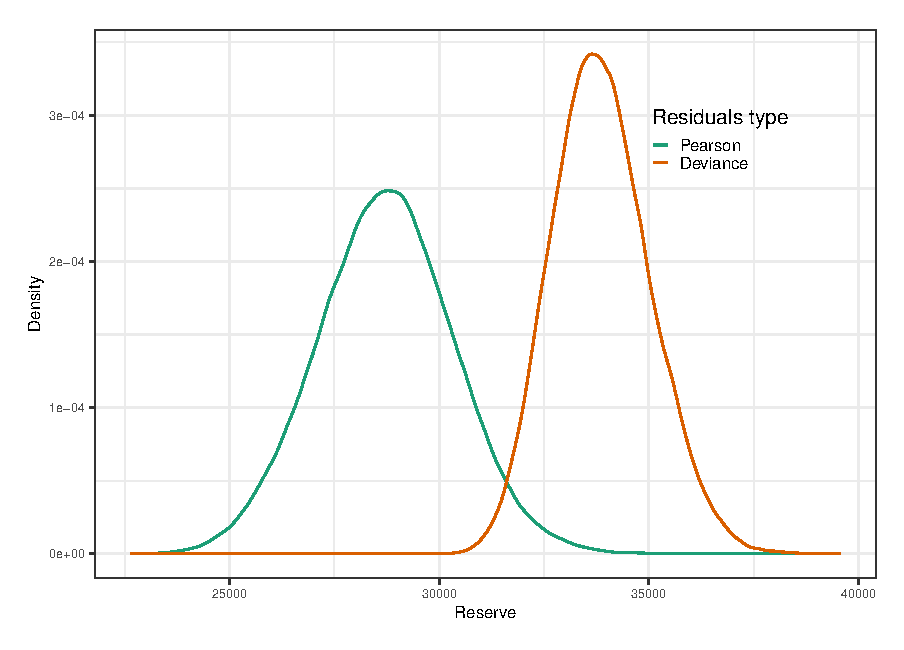
\includegraphics{pois_semiparam}
  \caption{Predictive distribution for different types of semiparameteric bootstrap}
  \label{fig:pred-semiparam}
\end{figure}

\newgeometry{bottom=0.1cm}

\chapter{Simulation study}

\epstopdfsetup{outdir=/home/othman/repos/masters_thesis/plots/}

As mentioned in the \nameref{intro} and \cref{sec:boot-proc}, we want to investigate the effect of deviations from the model assumptions on the predictive distribution of the total outstanding claims. To this end, we simulate a large number of run-off triangles which conform perfectly to these assumptions, perturb them in a number of ways, and use the bootstrap methods described in \cref{chapter:mack,chapter:poisson} to compute resulting distribution. We broadly follow the methodology outlined in \cite{schiegl}, adapted, of course, to the models under consideration.

\section{Mack's model} \label{sec:mack-sim}

Recall from \cref{sec:mack-intro} that \modelref{model:mack} is recursive in nature, with the cumulative claim amounts in the next development determined by the observations in the previous one, and therefore requires that the first column of the triangle already be given in some way. We could use a seperate model to generate this, but we choose here to simply take the one from the UK Motor dataset in \cref{tab:uk-motor}. Likewise, we will use as development factors $f_1, \dots, f_{I - 1}$ and dispersion parameters $\sigma_1, \dots, \sigma_{I - 1}$ the fitted ones for this triangle. To generate a triangle which perfectly satisfies \cref{assump:mack-expectation,assump:mack-variance,assump:mack-independence}, we can then start from the initial column and use any suitable data-generating process (such as \cref{eq:time-series-model}) to recursively simulate the following columns of the triangle, as outline in \cref{alg:clean-mack-triangle}.

\begin{algorithm}[!htb]
  \begin{algorithmic}
    \Require{Development factors $f_1, \dots, f_{I - 1}$, dispersion parameters $\sigma_1, \dots, \sigma_{I - 1}$}
    \ForAll{$1 \leq i \leq I$, $2 \leq j \leq I$}
      \State $C_{ij} \gets 0$
    \EndFor
    \For{$i \gets 1, I$}
      \State $C^*_{i1} \gets C_{i1}$
      \For{$j \gets 2, I + 1 - i$}
        \State $C^*_{ij} \gets \mathcal{N}(f_j C^*_{i, j - 1}, \sigma_j^2 C^*_{i, j - 1})$
      \EndFor
    \EndFor
    \State \Return{$(C^*_{ij})_{1 \leq i,j \leq I}$}
  \end{algorithmic}
  \caption{Simulating a clean triangle conforming to \modelref{model:mack}}
  \label{alg:clean-mack-triangle}
\end{algorithm}

\restoregeometry

This immediately suggests a way of producing triangles where the assumptions have been perturbed for a single point $(i^*, j^*)$ with $i^* + j^* \leq I + 1$ and $j^* > 1$. In the contaminated row, we start from the first column and recursively simulate observations until we arrive at column $j^*$. Using perturbation factors $c_\mu$ and $c_\sigma$ for the mean and variance, we then draw an observation from the perturbed distribution $\mathcal{N}(c_\mu f_{j^* - 1} C^*_{i^*, j^* - 1}, c_\sigma \sigma^2_{j^* - 1} C^*_{i^*, j^* - 1})$. The non-contaminated rows are then obtained with the same procedure as in \cref{alg:clean-mack-triangle}.

\begin{algorithm}[!htb]
  \begin{algorithmic}
    \Require{Development factors $f_1, \dots, f_{I - 1}$, dispersion parameters $\sigma_1, \dots, \sigma_{I - 1}$, perturbed point $(i^*, j^*)$ with $i^* + j^* \leq I + 1$ and $j^* > 1$, perturbation factors $c_\mu$, $c_\sigma$}
    \ForAll{$1 \leq i, j \leq I$}
      \State $C_{ij} \gets 0$
    \EndFor
    \For{$i \gets 1, I$}
      \State $C^*_{i1} \gets C_{i1}$
      \If{$i \neq i^*$}
        \For{$j \gets 2, I + 1 - i$}
          \State $C^*_{ij} \gets \mathcal{N}(f_j C^*_{i, j - 1}, \sigma_j^2 C^*_{i, j - 1})$
        \EndFor
      \Else
        \For{$j \gets 1, j^* - 1$}
          \State $C^*_{i^*j} \gets \mathcal{N}(f_j C^*_{i^*, j - 1}, \sigma_j^2 C^*_{i^*, j - 1})$
        \EndFor
        \State $C^*_{i^*j^*} \gets \mathcal{N}(c_\mu \, f_j C^*_{i^*, j^* - 1}, c_\sigma \, \sigma_j^2 C^*_{i^*, j^* - 1})$
        \For{$j \gets j^* + 1, I$}
          \State $C^*_{i^*j} \gets \mathcal{N}(f_j C^*_{i^*, j - 1}, \sigma_j^2 C^*_{i^*, j - 1})$
        \EndFor
      \EndIf
    \EndFor
    \State \Return{$(C^*_{ij})_{1 \leq i,j \leq I}$}
  \end{algorithmic}
  \caption{Simulating triangle with single perturbed point for \modelref{model:mack}}
  \label{alg:pert-mack-triangle}
\end{algorithm}

We can obtain algorithms for simulating triangles where an entire origin or calendar period has been perturbed in a similar way.

\section{Overdispersed Poisson GLM} \label{sec:odp-sim}

Simulating triangles conforming to \modelref{model:odp} is significantly easier than for \modelref{model:mack}, as we don't have to deal with recursion. Using the fitted parameters from \cref{tab:uk-motor-long} for $\phi$, $c$, $a_1, \dots, a_I$ and $b_1, \dots, b_I$, we generate an observation for every cell $(i, j)$ in the upper triangle by drawing from an appropriate distribution, as shown in \cref{alg:clean-odp-triangle}.

\begin{algorithm}[H]
  \begin{algorithmic}
    \Require{Intercept $c$, development period parameters $a_2, \dots, a_I$, origin period parameters $b_2, \dots, b_I$, dispersion parameter $\phi$}
    \State $a_1 \gets 0$, $b_1 \gets 0$
    \ForAll{$1 \leq i, j \leq I$}
      \State $\mu_{ij} \gets \exp(c + a_i + b_j)$
      \State $X_{ij} \gets 0$
    \EndFor
    \For{$i \gets 1, I$}
      \For{$j \gets 1, I + 1 - i$}
        \State $X^*_{ij} \gets \mathcal{N}(\mu_{ij}, \sqrt{\phi \mu_{ij}})$
      \EndFor
    \EndFor
    \State \Return{$(X^*_{ij})_{1 \leq i,j \leq I}$}
  \end{algorithmic}
  \caption{Simulating a clean triangle conforming to \modelref{model:odp}}
  \label{alg:clean-odp-triangle}
\end{algorithm}

Triangles with a single perturbed point can then be obtained straightforwardly from this.

\begin{algorithm}[H]
  \begin{algorithmic}
    \Require{Intercept $c$, development period parameters $a_2, \dots, a_I$, origin period parameters $b_2, \dots, b_I$, dispersion parameter $\phi$, perturbation factor $c_\lambda$}
    \State $a_1 \gets 0$, $b_1 \gets 0$
    \ForAll{$1 \leq i, j \leq I$}
      \State $\mu_{ij} \gets \exp(c + a_i + b_j)$
      \State $X_{ij} \gets 0$
    \EndFor
    \For{$i \gets 1, I$}
      \For{$j \gets 1, I + 1 - i$}
        \State $X^*_{ij} \gets \mathcal{N}(\mu_{ij}, \sqrt{\phi \mu_{ij}})$
      \EndFor
    \EndFor
    \State \Return{$(X^*_{ij})_{1 \leq i,j \leq I}$}
  \end{algorithmic}
  \caption{Simulating triangle with single perturbed point for \modelref{model:odp}}
  \label{alg:pert-odp-triangle}
\end{algorithm}

Again, similar algorithms can be used for perturbed origin or calendar periods.

\section{Setup}

We are now ready to discuss the general setup of the simulation. Using \cref{alg:pert-mack-triangle,alg:pert-odp-triangle}, we generate claims triangles which perfectly satisfy the assumptions of \modelref{model:mack} or \modelref{model:odp} except for a selected number of points. In particular, we consider the three cases of
\begin{inparaenum}[(i)]
  \item a single perturbed observation
  \item a perturbed calendar period and
  \item a perturbed origin period.
\end{inparaenum}
In each instance, we carry out one of the bootstrap procedures outlined in \cref{chapter:mack,chapter:poisson} while excluding a subset of observations of the same type as the contaminated one, and then compare the resulting predictive distributions. Our hope is that we can detect a significant difference between the predictive distribution obtained when excluding the right subset and the ones where a different subset has been removed. This would then suggest a way of detecting irregularities in new triangles: compare for every point, calendar period or origin period the predictive bootstrap distribution obtained with and without this point; if a significant difference can be detected, then this subset constitutes a deviation from the model.

The way in which observations can be excluded when carrying out the bootstrap is specific to each method, and raises a number of practical issues. For the semiparametric bootstraps, the obvious way of excluding observations is to simply remove the corresponding residuals from the resampling pool. In the case of \modelref{model:mack}, this implies that the first column cannot contain contaminated points. This makes sense, as \modelref{model:mack} does not make any statements regarding the behaviour of the initial observations. While odd points in the triangle may be considered \emph{outliers} in a general sense, they do not necessarily constitute deviations from the model assumptions. To minimise the impact of this extraneous factor on the results, we have taken the approach of borrowing this initial column from the benchmark dataset in \cref{tab:uk-motor}, as explained in \cref{sec:mack-sim}.

For the parametric bootstrap, is is not as clear how we should go about excluding certain points. Obviously, our goal is to nullify the impact of these observations on the bootstrap result, which suggests removing them from the initial fitting process when obtaining the parametric model used to simulate new pseudo-data. We have to be careful here, however, as this can sometimes lead to situations where the model cannot be fit at all. In particular, for \modelref{model:mack}, we cannot exclude the upper right corner point, because we cannot estimate the final development factor otherwise. The approach outlined here is therefore not suitable to detecting deviations for this point. This is no great loss, however: the final development year requires special attention in any case, as it is very tied up with issues of tail factors and extrapolation. For \modelref{model:poisson}, the restriction is even more stringent; here, we cannot exclude the lower left corner either, because the resulting model would have no parameter corresponding to the final origin period, and consequently cannot be used for projection.

\section{Implementation and results}

The code for carrying out the simulations (as well as generating the examples from previous chapters) is mostly implemented in the \texttt{R} language \cite{R}. The most numerically intensive parts are written in \texttt{Fortran} and linked to the \texttt{R} code through a \texttt{C++} wrapper using the \texttt{Rcpp} package. For reproducibility and convenience, all code has been bundled together into a package which can be easily downloaded and used.

The results are presented as a series of faceted density plots comparing, for different configurations, the predictive density of the reserve when the contaminated observations have been excluded (shown in red) with the predictive densities obtained after excluding model-conforming points. The faceting variables are the indices of the outlying point(s). Owing to the large number of possible simulation options, it would be impractical to show all of them. We have therefore endeavoured to include a sample of the most interesting ones. The reader is encouraged to download the code using the instructions outlined previously and experiment with it for him- or herself.

\subsection{Mack's model}

For a single contaminated point, we observe poor performance of the conditional bootstrap accross the board. Referring to \Cref{fig:mack-sim-cond-semiparam,fig:mack-sim-cond-param}, we observe no significant difference between the predictive distribution with and without the contaminated point under a conditional bootstrap. By comparison, unconditional bootstraps perform a lot better, as can be seen in \Cref{fig:mack-sim-uncond-param-gamma,fig:mack-sim-uncond-param-normal,fig:mack-sim-uncond-semiparam-standard,fig:mack-sim-uncond-semiparam-student}. Intuitively, this makes sense, as the unconditional approach propagates resampled values further in the triangle (see \Cref{alg:uncond-semiparam-mack}), thus allowing perturbations to accumulate. It is somewhat surprising, however, that this should result in such a drastic difference, perhaps lending credence to the misgivings about the conditional approach outlined at the end of \Cref{sec:mack-challenge}. The diffference between contaminated and uncontaminated predictive distributions tends to be more pronounced for later development periods.

\newgeometry{bottom=0cm}

%% single
% residuals cond standardised
\begin{landscape}
  \begin{figure}
    \centering
    \includegraphics{mack_single_densities_cond_residuals_standardised_1}
    \caption{Single point contamination Mack model simulation results for the conditional semiparametric bootstrap with standardised residuals, $c_\mu = c_\sigma = 0.75$}
    \label{fig:mack-single-cond-semiparam}
  \end{figure}
\end{landscape}

\begin{landscape}
  \begin{figure}
    \ContinuedFloat
    \captionsetup{list=off,format=cont}
    \centering
    \includegraphics{mack_single_densities_cond_residuals_standardised_2}
    \caption{Single point contamination Mack model simulation results for the conditional semiparametric bootstrap with standardised residuals, $c_\mu = c_\sigma = 0.75$}
  \end{figure}
\end{landscape}

% residuals uncond standardised
\begin{landscape}
  \begin{figure}
    \centering
    \includegraphics{mack_single_densities_uncond_residuals_standardised_1}
    \caption{Single point contamination Mack model simulation results for the unconditional semiparametric bootstrap with standardised residuals, $c_\mu = c_\sigma = 0.75$}
    \label{fig:mack-single-uncond-semiparam-standard}
  \end{figure}
\end{landscape}

\begin{landscape}
  \begin{figure}
    \ContinuedFloat
    \captionsetup{list=off,format=cont}
    \centering
    \includegraphics{mack_single_densities_uncond_residuals_standardised_2}
    \caption{Single point contamination Mack model simulation results for the unconditional semiparametric bootstrap with standardised residuals, $c_\mu = c_\sigma = 0.75$}
  \end{figure}
\end{landscape}

% residuals uncond studentised
\begin{landscape}
  \begin{figure}
    \centering
    \includegraphics{mack_single_densities_uncond_residuals_studentised_1}
    \caption{Single point contamination Mack model simulation results for the unconditional semiparametric bootstrap with studentised residuals, $c_\mu = c_\sigma = 0.75$}
    \label{fig:mack-single-uncond-semiparam-student}
  \end{figure}
\end{landscape}

\begin{landscape}
  \begin{figure}
    \ContinuedFloat
    \captionsetup{list=off,format=cont}
    \centering
    \includegraphics{mack_single_densities_uncond_residuals_studentised_2}
    \caption{Single point contamination Mack model simulation results for the unconditional semiparametric bootstrap with studentised residuals, $c_\mu = c_\sigma = 0.75$}
  \end{figure}
\end{landscape}

% parametric cond normal
\begin{landscape}
  \begin{figure}
    \centering
    \includegraphics{mack_single_densities_cond_parametric_normal_1}
    \caption{Single point contamination Mack model simulation results for the conditional parametric bootstrap with normal distribution, $c_\mu = c_\sigma = 0.75$}
    \label{fig:mack-single-cond-param}
  \end{figure}
\end{landscape}

\begin{landscape}
  \begin{figure}
    \ContinuedFloat
    \captionsetup{list=off,format=cont}
    \centering
    \includegraphics{mack_single_densities_cond_parametric_normal_2}
    \caption{Single point contamination Mack model simulation results for the conditional parametric bootstrap with normal distribution, $c_\mu = c_\sigma = 0.75$}
  \end{figure}
\end{landscape}

% parametric uncond normal
\begin{landscape}
  \begin{figure}
    \centering
    \includegraphics{mack_single_densities_uncond_parametric_normal_1}
    \caption{Single point contamination Mack model simulation results for the unconditional parametric bootstrap with normal distribution, $c_\mu = c_\sigma = 0.75$}
    \label{fig:mack-single-uncond-param-normal}
  \end{figure}
\end{landscape}

\begin{landscape}
  \begin{figure}
    \ContinuedFloat
    \captionsetup{list=off,format=cont}
    \centering
    \includegraphics{mack_single_densities_uncond_parametric_normal_2}
    \caption{Single point contamination Mack model simulation results for the unconditional parametric bootstrap with normal distribution, $c_\mu = c_\sigma = 0.75$}
  \end{figure}
\end{landscape}

% parametric uncond gamma
\begin{landscape}
  \begin{figure}
    \centering
    \includegraphics{mack_single_densities_uncond_parametric_gamma_1}
    \caption{Single point contamination Mack model simulation results for the unconditional parametric bootstrap with gamma distribution, $c_\mu = c_\sigma = 0.75$}
    \label{fig:mack-single-uncond-param-gamma}
  \end{figure}
\end{landscape}

\begin{landscape}
  \begin{figure}
    \ContinuedFloat
    \captionsetup{list=off,format=cont}
    \centering
    \includegraphics{mack_single_densities_uncond_parametric_gamma_2}
    \caption{Single point contamination Mack model simulation results for the unconditional parametric bootstrap with gamma distribution, $c_\mu = c_\sigma = 0.75$}
  \end{figure}
\end{landscape}

%% calendar
% residuals cond standardised
\begin{landscape}
  \begin{figure}
    \centering
    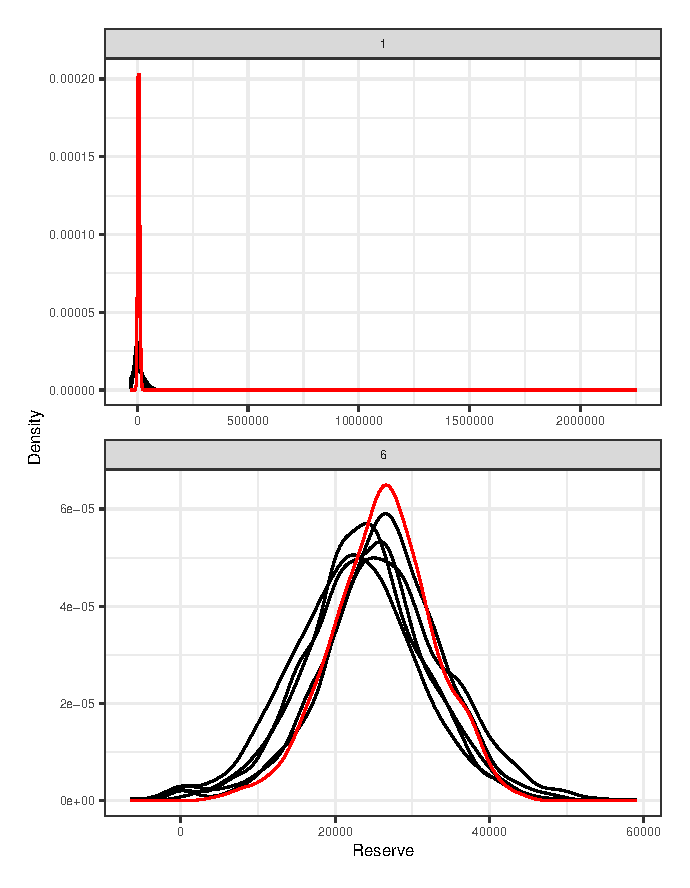
\includegraphics{mack_calendar_densities_cond_residuals_standardised}
    \caption{Calendar period contamination Mack model simulation results for the conditional semiparametric bootstrap with standardised residuals, $c_\mu = c_\sigma = 0.75$}
    \label{fig:mack-calendar-cond-semiparam}
  \end{figure}
\end{landscape}

% residuals uncond standardised
\begin{landscape}
  \begin{figure}
    \centering
    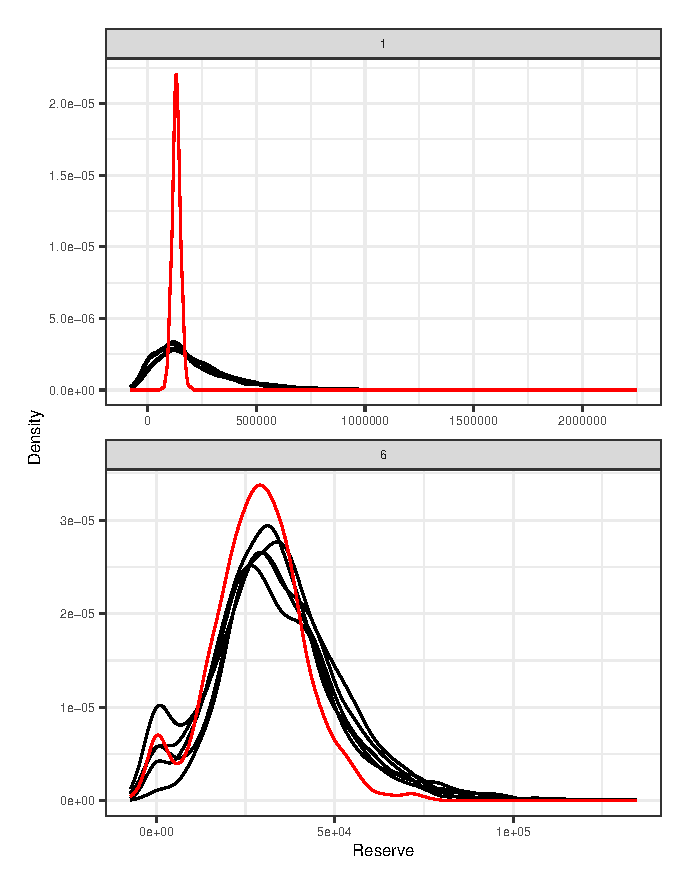
\includegraphics{mack_calendar_densities_uncond_residuals_standardised}
    \caption{Calendar period contamination Mack model simulation results for the unconditional semiparametric bootstrap with standardised residuals, $c_\mu = c_\sigma = 0.75$}
    \label{fig:mack-calendar-uncond-semiparam-standard}
  \end{figure}
\end{landscape}

% residuals uncond studentised
\begin{landscape}
  \begin{figure}
    \centering
    \includegraphics{mack_calendar_densities_uncond_residuals_studentised}
    \caption{Calendar period contamination Mack model simulation results for the unconditional semiparametric bootstrap with studentised residuals, $c_\mu = c_\sigma = 0.75$}
    \label{fig:mack-calendar-uncond-semiparam-student}
  \end{figure}
\end{landscape}

% parametric cond normal
\begin{landscape}
  \begin{figure}
    \centering
    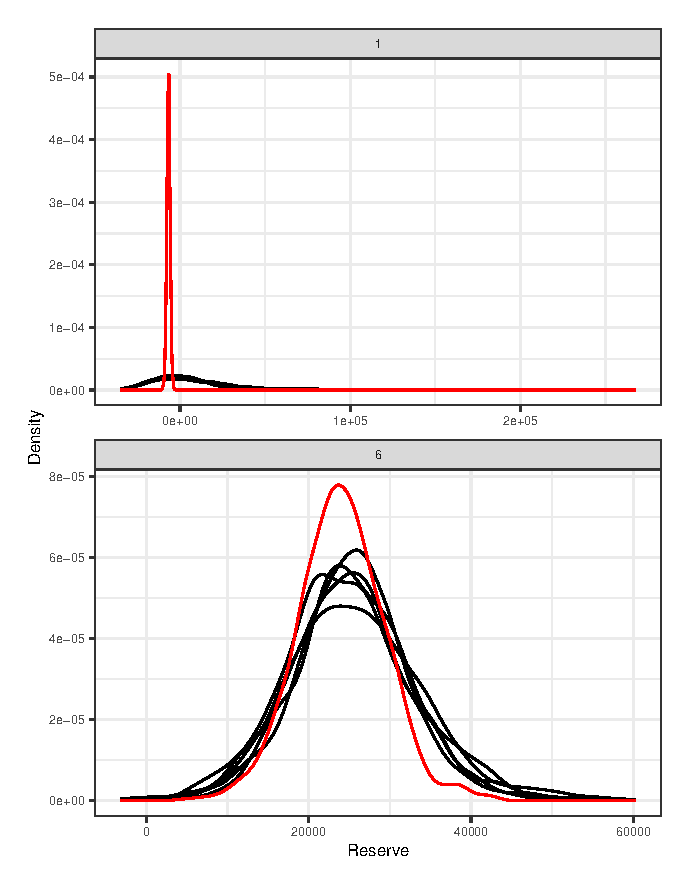
\includegraphics{mack_calendar_densities_cond_parametric_normal}
    \caption{Calendar period contamination Mack model simulation results for the conditional parametric bootstrap with normal distribution, $c_\mu = c_\sigma = 0.75$}
    \label{fig:mack-calendar-cond-param}
  \end{figure}
\end{landscape}

% parametric uncond normal
\begin{landscape}
  \begin{figure}
    \centering
    \includegraphics{mack_calendar_densities_uncond_parametric_normal}
    \caption{Calendar period contamination Mack model simulation results for the unconditional parametric bootstrap with normal distribution, $c_\mu = c_\sigma = 0.75$}
    \label{fig:mack-calendar-uncond-param-normal}
  \end{figure}
\end{landscape}

% parametric uncond gamma
\begin{landscape}
  \begin{figure}
    \centering
    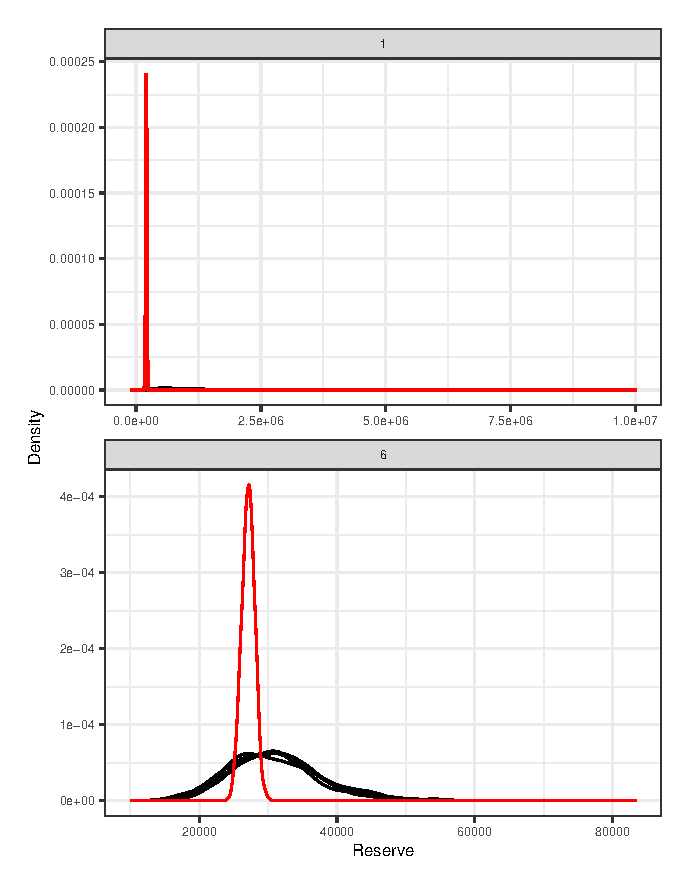
\includegraphics{mack_calendar_densities_uncond_parametric_gamma}
    \caption{Calendar period contamination Mack model simulation results for the unconditional parametric bootstrap with gamma distribution, $c_\mu = c_\sigma = 0.75$}
    \label{fig:mack-calendar-uncond-param-gamma}
  \end{figure}
\end{landscape}

%% origin
% residuals cond standardised
\begin{landscape}
  \begin{figure}
    \centering
    \includegraphics{mack_origin_densities_cond_residuals_standardised}
    \caption{Origin period contamination Mack model simulation results for the conditional semiparametric bootstrap with standardised residuals, $c_\mu = c_\sigma = 0.75$}
    \label{fig:mack-origin-cond-semiparam}
  \end{figure}
\end{landscape}

% residuals uncond standardised
\begin{landscape}
  \begin{figure}
    \centering
    \includegraphics{mack_origin_densities_uncond_residuals_standardised}
    \caption{Origin period contamination Mack model simulation results for the unconditional semiparametric bootstrap with standardised residuals, $c_\mu = c_\sigma = 0.75$}
    \label{fig:mack-origin-uncond-semiparam-standard}
  \end{figure}
\end{landscape}

% residuals uncond studentised
\begin{landscape}
  \begin{figure}
    \centering
    \includegraphics{mack_origin_densities_uncond_residuals_studentised}
    \caption{Origin period contamination Mack model simulation results for the unconditional semiparametric bootstrap with studentised residuals, $c_\mu = c_\sigma = 0.75$}
    \label{fig:mack-origin-uncond-semiparam-student}
  \end{figure}
\end{landscape}

% parametric cond normal
\begin{landscape}
  \begin{figure}
    \centering
    \includegraphics{mack_origin_densities_cond_parametric_normal}
    \caption{Origin period contamination Mack model simulation results for the conditional parametric bootstrap with normal distribution, $c_\mu = c_\sigma = 0.75$}
    \label{fig:mack-origin-cond-param}
  \end{figure}
\end{landscape}

% parametric uncond normal
\begin{landscape}
  \begin{figure}
    \centering
    \includegraphics{mack_origin_densities_uncond_parametric_normal}
    \caption{Origin period contamination Mack model simulation results for the unconditional parametric bootstrap with normal distribution, $c_\mu = c_\sigma = 0.75$}
    \label{fig:mack-origin-uncond-param-normal}
  \end{figure}
\end{landscape}

% parametric uncond gamma
\begin{landscape}
  \begin{figure}
    \centering
    \includegraphics{mack_origin_densities_uncond_parametric_gamma}
    \caption{Origin period contamination Mack model simulation results for the unconditional parametric bootstrap with gamma distribution, $c_\mu = c_\sigma = 0.75$}
    \label{fig:mack-origin-uncond-param-gamma}
  \end{figure}
\end{landscape}

\restoregeometry

\subsection{Overdispersed Poisson GLM}

poor performance for the residuals bootstrap: removing the offending point produces absolutely no difference in the predictive distribution of the reserve. Investigation reveals that this is caused by the fact that model

The parametric bootstrap, on the other hand, performs considerably better.

\newgeometry{bottom=0cm}

%% single
% parametric gamma
\begin{landscape}
  \begin{figure}
    \centering
    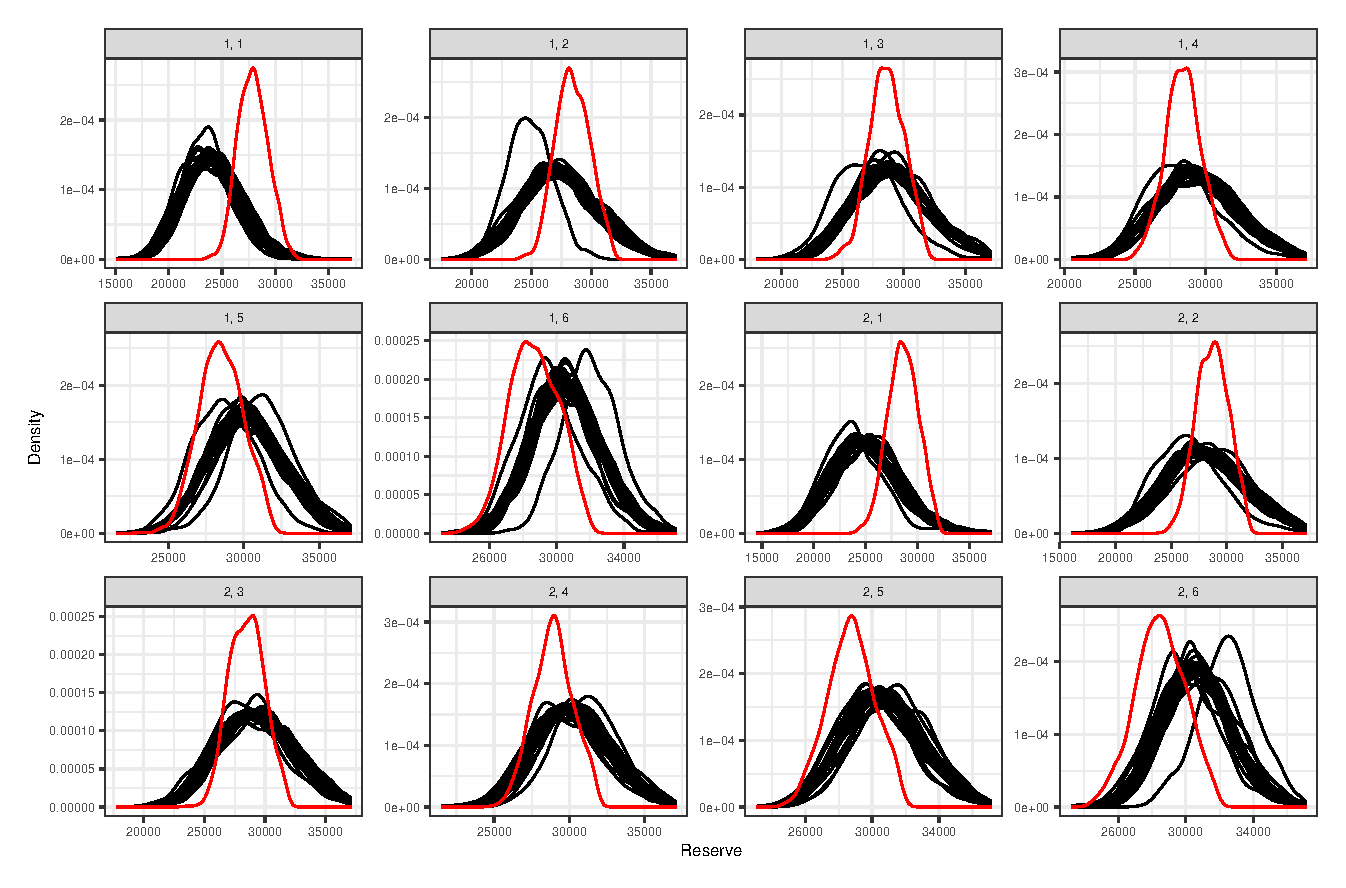
\includegraphics{glm_single_densities_parametric_gamma_1}
    \caption{Single point contamination ODP model simulation results for the parametric bootstrap with gamma distribution, $c_\lambda = 2$}
    \label{fig:glm-single-param-gamma}
  \end{figure}
\end{landscape}

\begin{landscape}
  \begin{figure}
    \ContinuedFloat
    \captionsetup{list=off,format=cont}
    \centering
    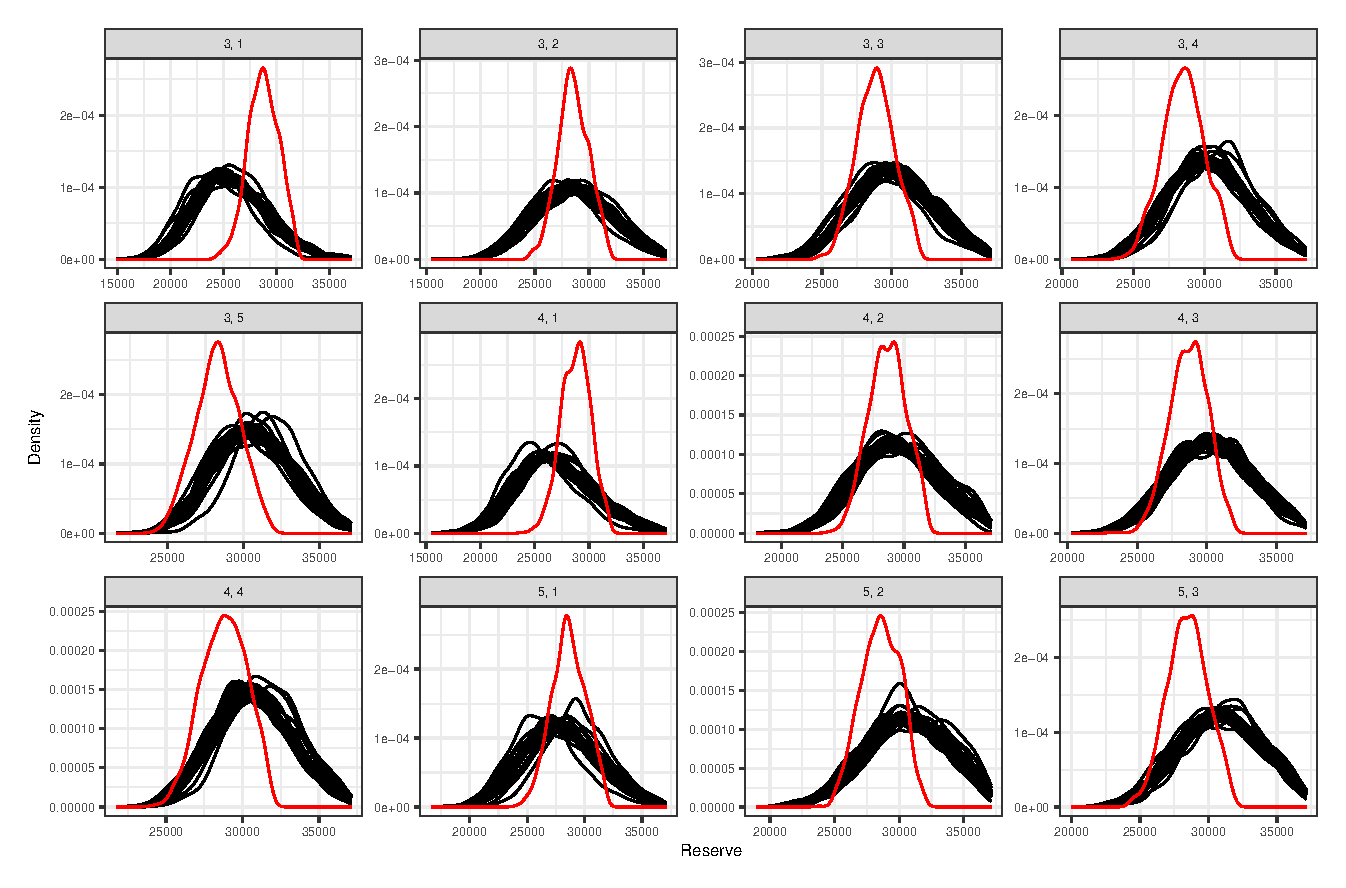
\includegraphics{glm_single_densities_parametric_gamma_2}
    \caption{Single point contamination ODP model simulation results for the parametric bootstrap with gamma distribution, $c_\lambda = 2$}
  \end{figure}
\end{landscape}

% parametric normal
\begin{landscape}
  \begin{figure}
    \centering
    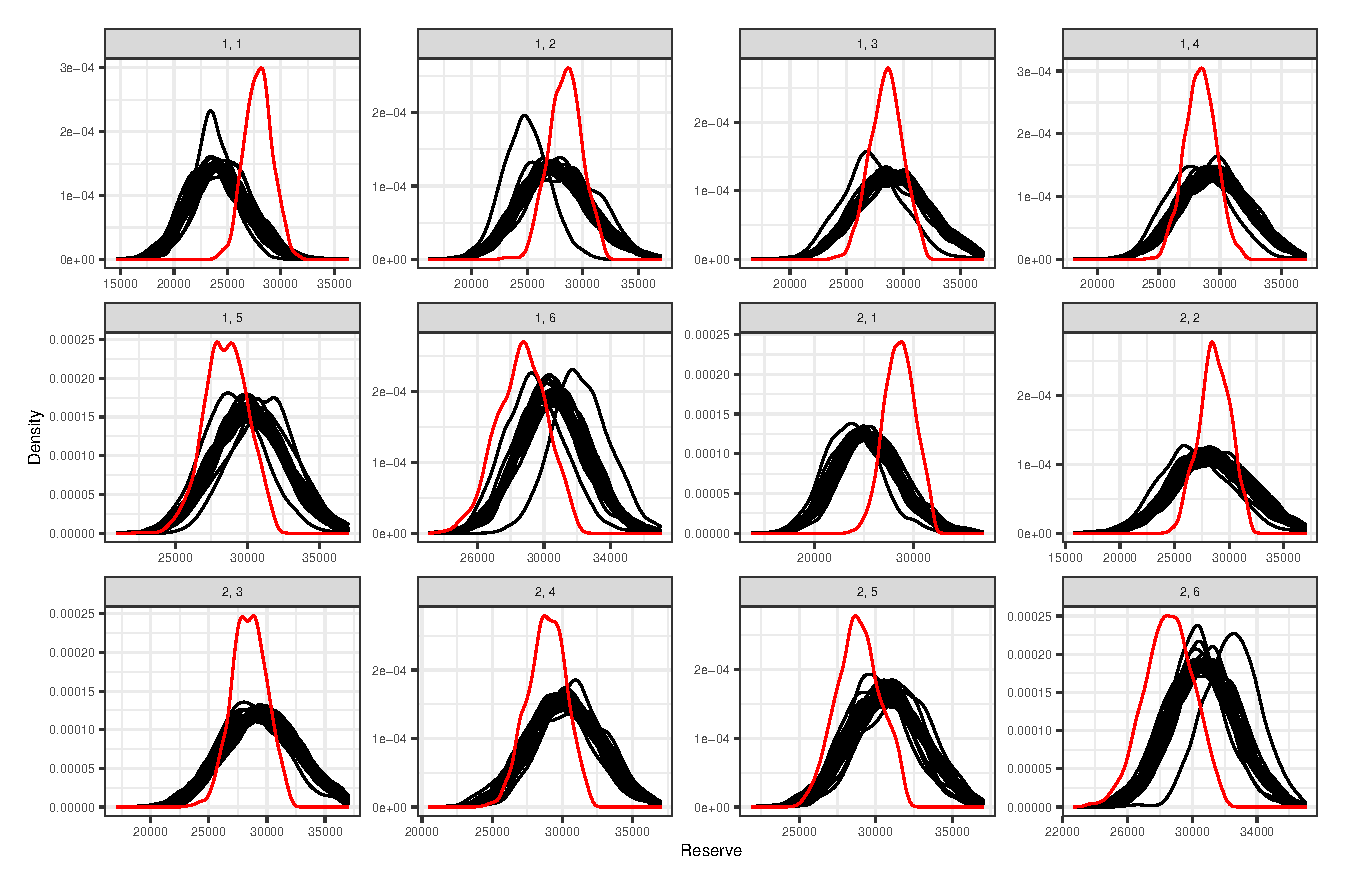
\includegraphics{glm_single_densities_parametric_normal_1}
    \caption{Single point contamination ODP model simulation results for the parametric bootstrap with normal distribution, $c_\lambda = 2$}
    \label{fig:glm-single-param-norm}
  \end{figure}
\end{landscape}

\begin{landscape}
  \begin{figure}
    \ContinuedFloat
    \captionsetup{list=off,format=cont}
    \centering
    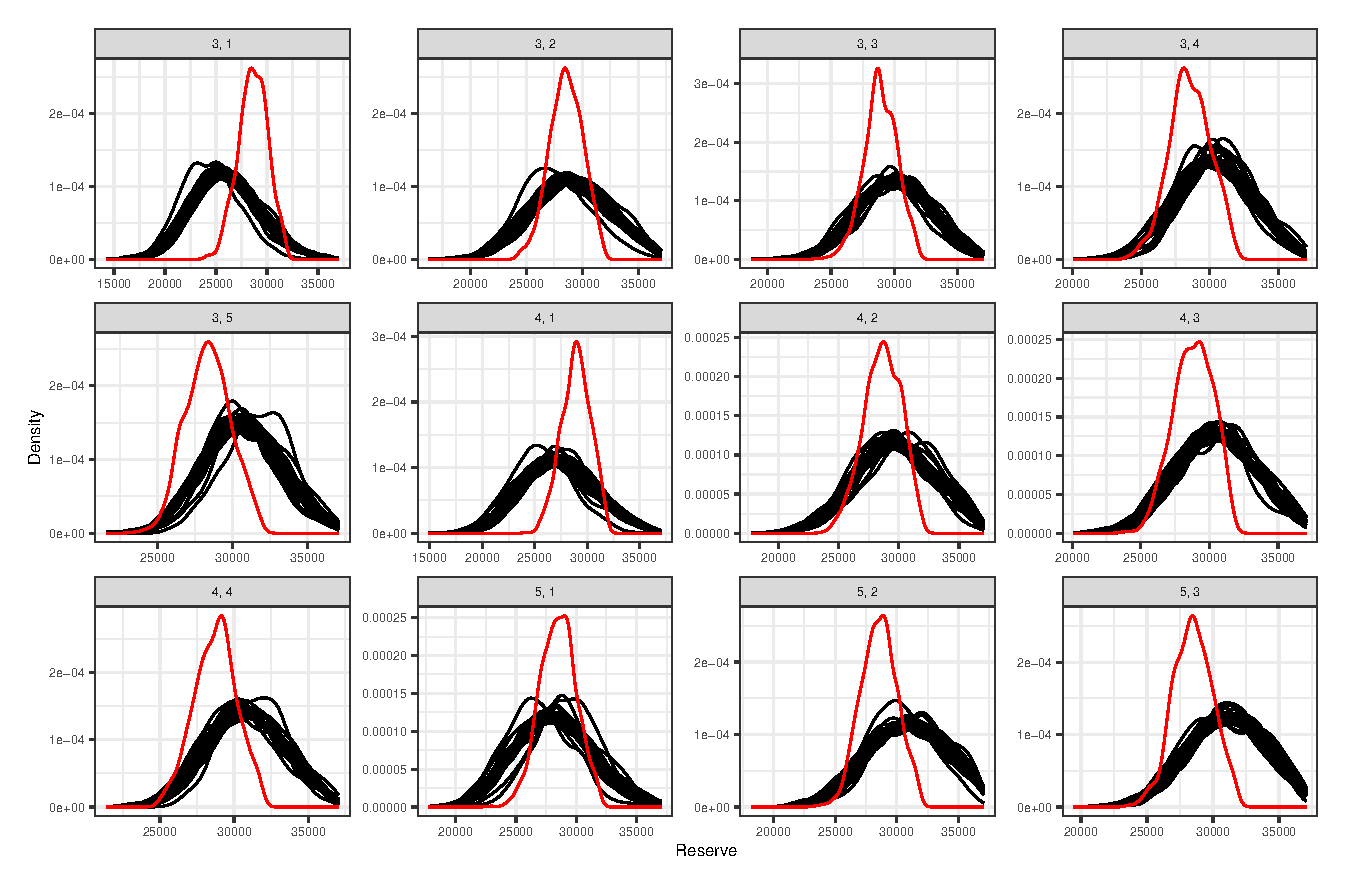
\includegraphics{glm_single_densities_parametric_normal_2}
    \caption{Single point contamination ODP model simulation results for the parametric bootstrap with normal distribution, $c_\lambda = 2$}
  \end{figure}
\end{landscape}

% parametric poisson
\begin{landscape}
  \begin{figure}
    \centering
    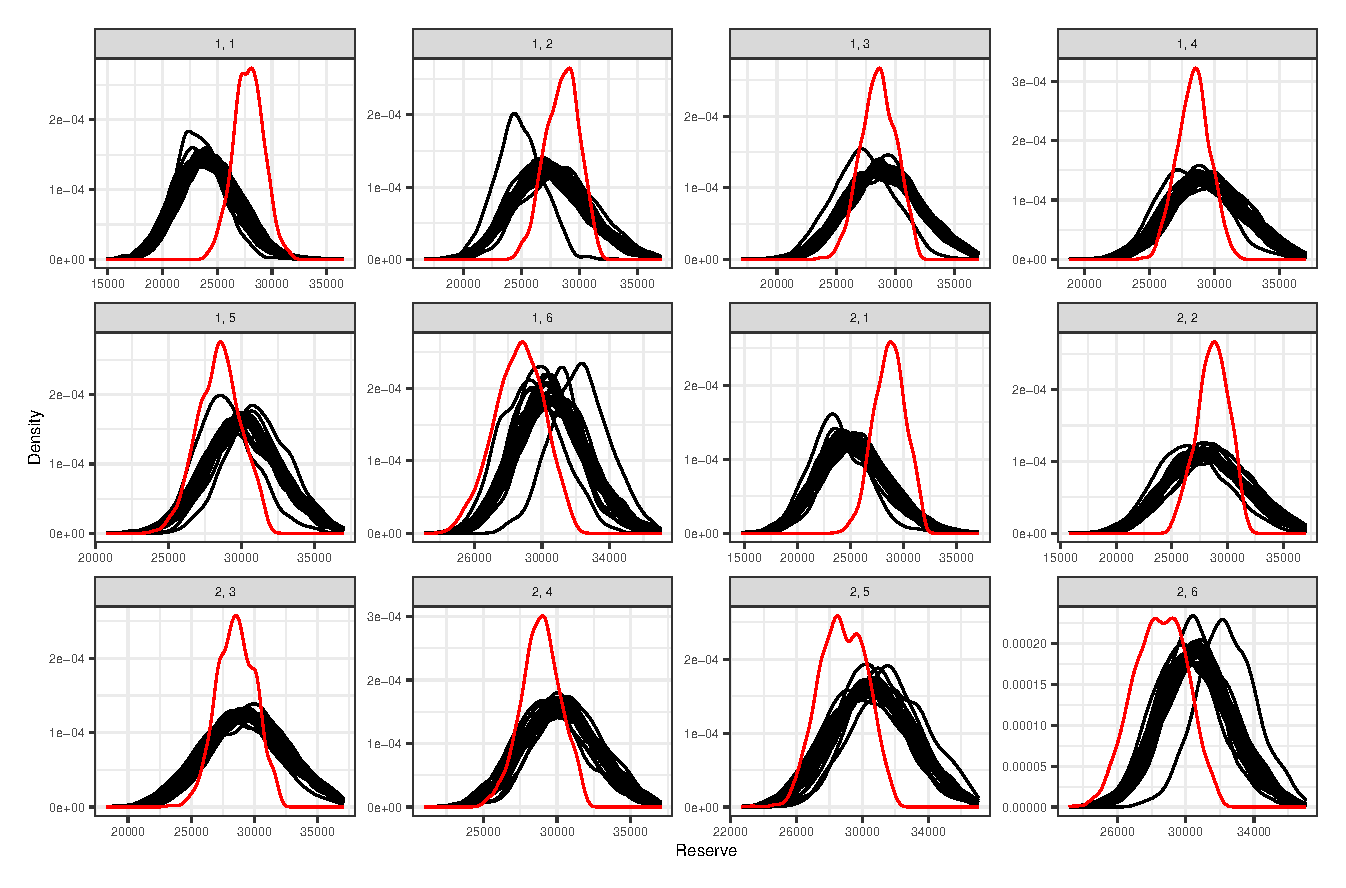
\includegraphics{glm_single_densities_parametric_poisson_1}
    \caption{Single point contamination ODP model simulation results for the parametric bootstrap with Poisson distribution, $c_\lambda = 2$}
    \label{fig:glm-single-param-pois}
  \end{figure}
\end{landscape}

\begin{landscape}
  \begin{figure}
    \ContinuedFloat
    \captionsetup{list=off,format=cont}
    \centering
    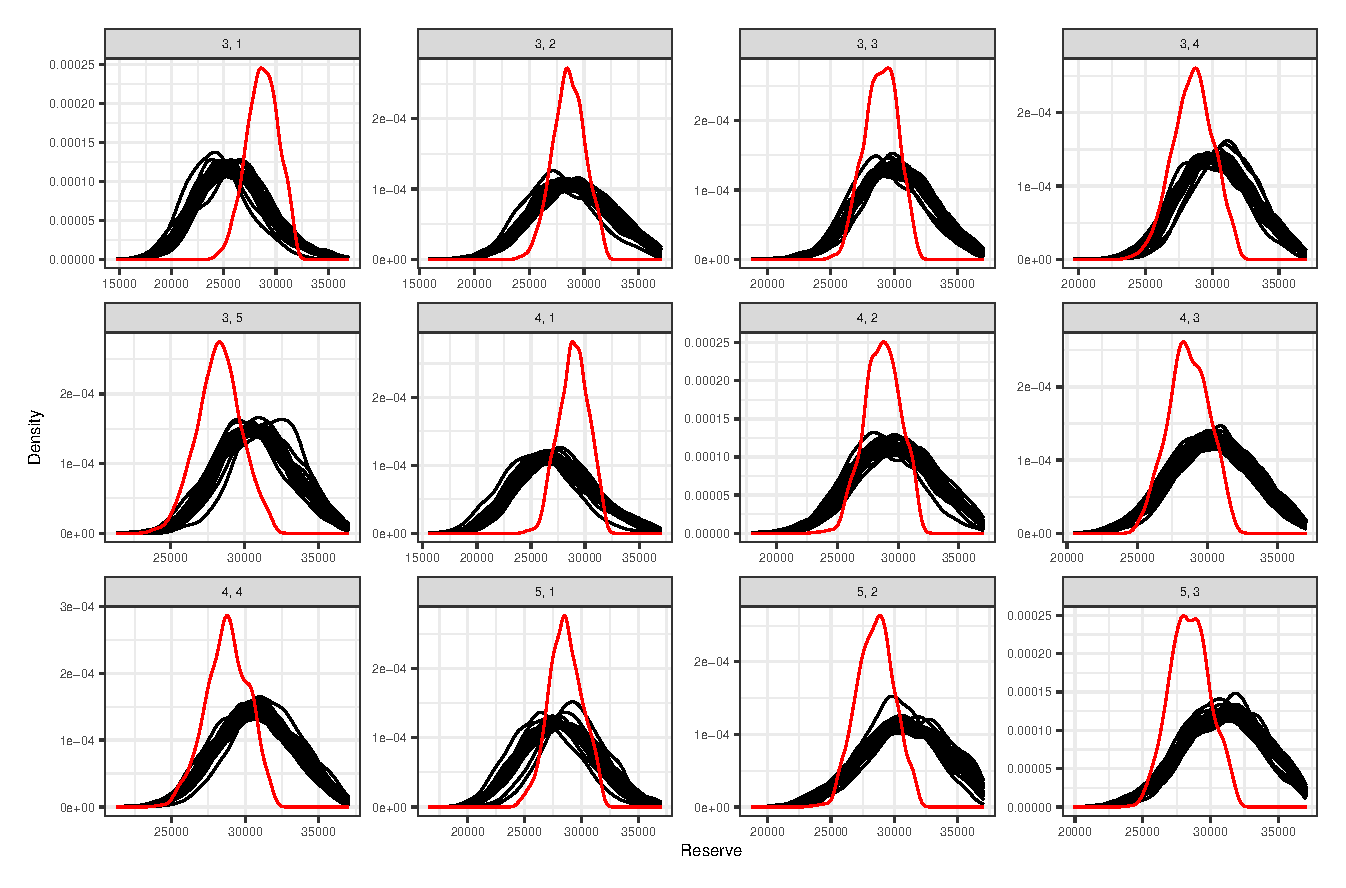
\includegraphics{glm_single_densities_parametric_poisson_2}
    \caption{Single point contamination ODP model simulation results for the parametric bootstrap with Poisson distribution, $c_\lambda = 2$}
  \end{figure}
\end{landscape}

% residuals
\begin{landscape}
  \begin{figure}
    \centering
    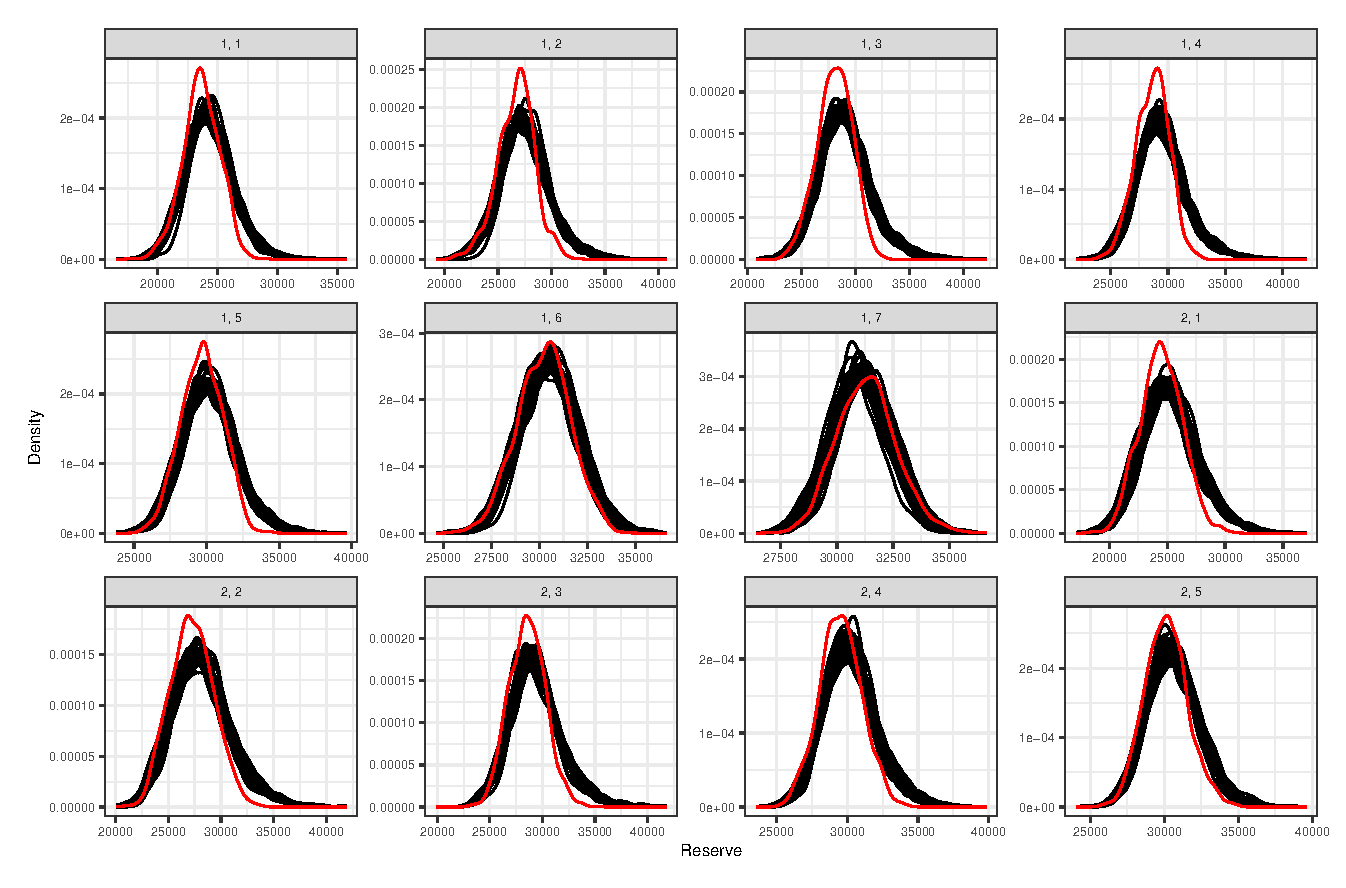
\includegraphics{glm_single_densities_residuals_1}
    \caption{Single point contamination ODP model simulation results for the semiparametric bootstrap with Pearson residuals, $c_\lambda = 2$}
    \label{fig:glm-single-semiparam}
  \end{figure}
\end{landscape}

\begin{landscape}
  \begin{figure}
    \ContinuedFloat
    \captionsetup{list=off,format=cont}
    \centering
    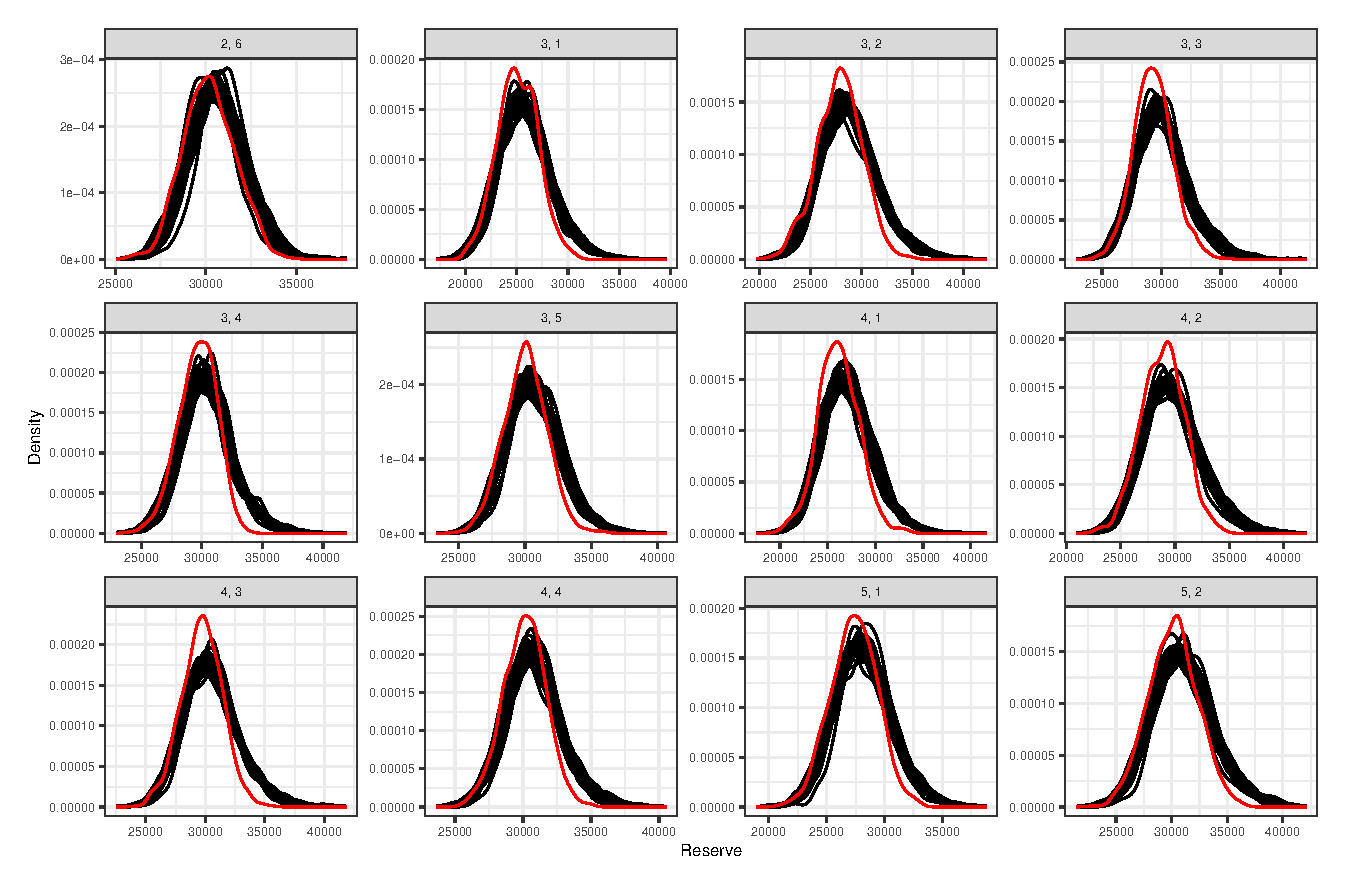
\includegraphics{glm_single_densities_residuals_2}
    \caption{Single point contamination ODP model simulation results for the semiparametric bootstrap with Pearson residuals, $c_\lambda = 2$}
  \end{figure}
\end{landscape}

% % different factors
% \begin{landscape}
%   \begin{figure}
%     \centering
%     \includegraphics{glm_single_by_factor}
%     \caption{Single point contamination ODP model simulation results for $i = j = 3$ and different values of $c_\lambda$. The predictive distribution based on the cleaned data is shown black.}
%     \label{fig:glm-single-by-factor}
%   \end{figure}
% \end{landscape}

%% calendar
% parametric gamma
\begin{landscape}
  \begin{figure}
    \centering
    \includegraphics{glm_calendar_densities_parametric_gamma}
    \caption{Calendar period contamination ODP model simulation results for the parametric bootstrap with gamma distribution, $c_\lambda = 2$}
    \label{fig:glm-calendar-param-gamma}
  \end{figure}
\end{landscape}

% parametric normal
\begin{landscape}
  \begin{figure}
    \centering
    \includegraphics{glm_calendar_densities_parametric_normal}
    \caption{Calendar period contamination ODP model simulation results for the parametric bootstrap with normal distribution, $c_\lambda = 2$}
    \label{fig:glm-calendar-param-norm}
  \end{figure}
\end{landscape}

% parametric poisson
\begin{landscape}
  \begin{figure}
    \centering
    \includegraphics{glm_calendar_densities_parametric_poisson}
    \caption{Calendar period contamination ODP model simulation results for the parametric bootstrap with Poisson distribution, $c_\lambda = 2$}
    \label{fig:glm-calendar-param-pois}
  \end{figure}
\end{landscape}

% residuals
\begin{landscape}
  \begin{figure}
    \centering
    \includegraphics{glm_calendar_densities_residuals}
    \caption{Calendar period contamination ODP model simulation results for the semiparametric bootstrap with Pearson residuals, $c_\lambda = 2$}
    \label{fig:glm-calendar-semiparam}
  \end{figure}
\end{landscape}

%% origin
% parametric gamma
\begin{landscape}
  \begin{figure}
    \centering
    \includegraphics{glm_origin_densities_parametric_gamma}
    \caption{Origin period ODP model simulation results for the parametric bootstrap with gamma distribution, $c_\lambda = 2$}
    \label{fig:glm-origin-param-gamma}
  \end{figure}
\end{landscape}

% parametric normal
\begin{landscape}
  \begin{figure}
    \centering
    \includegraphics{glm_origin_densities_parametric_normal}
    \caption{Origin period ODP model simulation results for the parametric bootstrap with normal distribution, $c_\lambda = 2$}
    \label{fig:glm-origin-param-norm}
  \end{figure}
\end{landscape}

% parametric poisson
\begin{landscape}
  \begin{figure}
    \centering
    \includegraphics{glm_origin_densities_parametric_poisson}
    \caption{Origin period ODP model simulation results for the parametric bootstrap with Poisson distribution, $c_\lambda = 2$}
    \label{fig:glm-origin-param-pois}
  \end{figure}
\end{landscape}

% residuals
\begin{landscape}
  \begin{figure}
    \centering
    \includegraphics{glm_origin_densities_residuals}
    \caption{Origin period ODP model simulation results for the semiparametric bootstrap with Pearson residuals, $c_\lambda = 2$}
    \label{fig:glm-origin-semiparam}
  \end{figure}
\end{landscape}

\restoregeometry

\backmatter%

\chapter{Conclusion} \label{conclusion}

\printbibliography%

\end{document}
